\pdftrailerid{}
\pdfinfoomitdate=1
\pdfsuppressptexinfo=15
\pdfgentounicode=1


\pdfglyphtounicode{angbracketleftBig}{27E8 FE02}
\pdfglyphtounicode{angbracketleftBigg}{27E8 FE04}
\pdfglyphtounicode{angbracketleftbig}{27E8 FE01}
\pdfglyphtounicode{angbracketleftbigg}{27E8 FE03}
\pdfglyphtounicode{angbracketrightBig}{27E9 FE02}
\pdfglyphtounicode{angbracketrightBigg}{27E9 FE04}
\pdfglyphtounicode{angbracketrightbig}{27E9 FE01}
\pdfglyphtounicode{angbracketrightbigg}{27E9 FE03}
\pdfglyphtounicode{arrowbt}{2193}
\pdfglyphtounicode{arrowdblbt}{21D3}
\pdfglyphtounicode{arrowdbltp}{21D1}
\pdfglyphtounicode{arrowhookleft}{21AA}
\pdfglyphtounicode{arrowhookright}{21A9}
\pdfglyphtounicode{arrowtp}{2191}
\pdfglyphtounicode{arrowvertex}{23D0}
\pdfglyphtounicode{arrowvertexdbl}{20E6}%
\pdfglyphtounicode{backslashBig}{005C FE02}
\pdfglyphtounicode{backslashBigg}{005C FE04}
\pdfglyphtounicode{backslashbig}{005C FE01}
\pdfglyphtounicode{backslashbigg}{005C FE03}
\pdfglyphtounicode{braceex}{23AA}
\pdfglyphtounicode{bracehtipdownleft}{23DF}%
\pdfglyphtounicode{bracehtipdownright}{23DF}%
\pdfglyphtounicode{bracehtipupleft}{23DE}%
\pdfglyphtounicode{bracehtipupright}{23DE}%
\pdfglyphtounicode{braceleftBig}{007B FE02}
\pdfglyphtounicode{braceleftBigg}{007B FE04}
\pdfglyphtounicode{braceleftbig}{007B FE01}
\pdfglyphtounicode{braceleftbigg}{007B FE03}
\pdfglyphtounicode{braceleftbt}{23A9}
\pdfglyphtounicode{braceleftmid}{23A8}
\pdfglyphtounicode{bracelefttp}{23A7}
\pdfglyphtounicode{bracerightBig}{007D FE02}
\pdfglyphtounicode{bracerightBigg}{007D FE04}
\pdfglyphtounicode{bracerightbig}{007D FE01}
\pdfglyphtounicode{bracerightbigg}{007D FE03}
\pdfglyphtounicode{bracerightbt}{23AD}
\pdfglyphtounicode{bracerightmid}{23AC}
\pdfglyphtounicode{bracerighttp}{23AB}
\pdfglyphtounicode{bracketleftBig}{005B FE02}
\pdfglyphtounicode{bracketleftBigg}{005B FE04}
\pdfglyphtounicode{bracketleftbig}{005B FE01}
\pdfglyphtounicode{bracketleftbigg}{005B FE03}
\pdfglyphtounicode{bracketleftbt}{23A3}
\pdfglyphtounicode{bracketleftex}{23A2}
\pdfglyphtounicode{bracketlefttp}{23A1}
\pdfglyphtounicode{bracketrightBig}{005D FE02}
\pdfglyphtounicode{bracketrightBigg}{005D FE04}
\pdfglyphtounicode{bracketrightbig}{005D FE01}
\pdfglyphtounicode{bracketrightbigg}{005D FE03}
\pdfglyphtounicode{bracketrightbt}{23A6}
\pdfglyphtounicode{bracketrightex}{23A5}
\pdfglyphtounicode{bracketrighttp}{23A4}
\pdfglyphtounicode{ceilingleftBig}{2308 FE02}
\pdfglyphtounicode{ceilingleftBigg}{2308 FE04}
\pdfglyphtounicode{ceilingleftbig}{2308 FE01}
\pdfglyphtounicode{ceilingleftbigg}{2308 FE03}
\pdfglyphtounicode{ceilingrightBig}{2309 FE02}
\pdfglyphtounicode{ceilingrightBigg}{2309 FE04}
\pdfglyphtounicode{ceilingrightbig}{2309 FE01}
\pdfglyphtounicode{ceilingrightbigg}{2309 FE03}
\pdfglyphtounicode{circledotdisplay}{2A00 FE02}
\pdfglyphtounicode{circledottext}{2A00 FE01}
\pdfglyphtounicode{circlemultiplydisplay}{2A02 FE02}
\pdfglyphtounicode{circlemultiplytext}{2A02 FE01}
\pdfglyphtounicode{circleplusdisplay}{2A01 FE02}
\pdfglyphtounicode{circleplustext}{2A01 FE01}
\pdfglyphtounicode{contintegraldisplay}{222E FE02}
\pdfglyphtounicode{contintegraltext}{222E FE01}
\pdfglyphtounicode{coproductdisplay}{2210 FE02}
\pdfglyphtounicode{coproducttext}{2210 FE01}
\pdfglyphtounicode{floorleftBig}{230A FE02}
\pdfglyphtounicode{floorleftBigg}{230A FE04}
\pdfglyphtounicode{floorleftbig}{230A FE01}
\pdfglyphtounicode{floorleftbigg}{230A FE03}
\pdfglyphtounicode{floorrightBig}{230B FE02}
\pdfglyphtounicode{floorrightBigg}{230B FE04}
\pdfglyphtounicode{floorrightbig}{230B FE01}
\pdfglyphtounicode{floorrightbigg}{230B FE03}
\pdfglyphtounicode{hatwide}{02C6 FE01}
\pdfglyphtounicode{hatwider}{02C6 FE02}
\pdfglyphtounicode{hatwidest}{02C6 FE03}
\pdfglyphtounicode{integraldisplay}{222B FE02}
\pdfglyphtounicode{integraltext}{222B FE01}
\pdfglyphtounicode{intersectiondisplay}{22C2 FE02}
\pdfglyphtounicode{intersectiontext}{22C2 FE01}
\pdfglyphtounicode{logicalanddisplay}{22C0 FE02}
\pdfglyphtounicode{logicalandtext}{22C0 FE01}
\pdfglyphtounicode{logicalordisplay}{22C1 FE02}
\pdfglyphtounicode{logicalortext}{22C1 FE01}
\pdfglyphtounicode{mapsto}{21A6}
\pdfglyphtounicode{parenleftBig}{0028 FE02}
\pdfglyphtounicode{parenleftBigg}{0028 FE04}
\pdfglyphtounicode{parenleftbig}{0028 FE01}
\pdfglyphtounicode{parenleftbigg}{0028 FE03}
\pdfglyphtounicode{parenleftbt}{239D}
\pdfglyphtounicode{parenleftex}{239C}
\pdfglyphtounicode{parenlefttp}{239B}
\pdfglyphtounicode{parenrightBig}{0029 FE02}
\pdfglyphtounicode{parenrightBigg}{0029 FE04}
\pdfglyphtounicode{parenrightbig}{0029 FE01}
\pdfglyphtounicode{parenrightbigg}{0029 FE03}
\pdfglyphtounicode{parenrightbt}{23A0}
\pdfglyphtounicode{parenrightex}{239F}
\pdfglyphtounicode{parenrighttp}{239E}
\pdfglyphtounicode{productdisplay}{220F FE02}
\pdfglyphtounicode{producttext}{220F FE01}
\pdfglyphtounicode{radicalBig}{221A FE02}
\pdfglyphtounicode{radicalBigg}{221A FE04}
\pdfglyphtounicode{radicalbig}{221A FE01}
\pdfglyphtounicode{radicalbigg}{221A FE03}
\pdfglyphtounicode{radicalbt}{23B7}%
\pdfglyphtounicode{radicaltp}{231C}%
\pdfglyphtounicode{radicalvertex}{20D3}%
\pdfglyphtounicode{slashBig}{002F FE02}
\pdfglyphtounicode{slashBigg}{002F FE04}
\pdfglyphtounicode{slashbig}{002F FE01}
\pdfglyphtounicode{slashbigg}{002F FE03}
\pdfglyphtounicode{summationdisplay}{2211 FE02}
\pdfglyphtounicode{summationtext}{2211 FE01}
\pdfglyphtounicode{tie}{2040}
\pdfglyphtounicode{tildewide}{02DC FE01}
\pdfglyphtounicode{tildewider}{02DC FE02}
\pdfglyphtounicode{tildewidest}{02DC FE03}
\pdfglyphtounicode{uniondisplay}{22C3 FE02}
\pdfglyphtounicode{unionmultidisplay}{2A04 FE02}
\pdfglyphtounicode{unionmultitext}{2A04 FE01}
\pdfglyphtounicode{unionsqdisplay}{2A06 FE02}
\pdfglyphtounicode{unionsqtext}{2A06 FE01}
\pdfglyphtounicode{uniontext}{22C3 FE01}
\pdfglyphtounicode{vextenddouble}{20E6}%
\pdfglyphtounicode{vextendsingle}{20D3}%

\documentclass[11pt]{article}
\usepackage[T1]{fontenc}
\usepackage[utf8]{inputenc}
\usepackage{lmodern}
\usepackage[margin=1in]{geometry}
\usepackage{amsmath,amssymb,amsthm,mathtools}
\usepackage{microtype,booktabs,longtable,array,enumitem}
\usepackage{tikz,tikz-cd}
\usetikzlibrary{arrows.meta,positioning,calc}
\usepackage{xcolor}
\usepackage{hyperref}
\hypersetup{colorlinks=true,linkcolor=blue!45!black,citecolor=blue!45!black,urlcolor=blue!45!black,pdftitle={The Kervaire invariant problem at the prime three},pdfauthor={OpenAI}}
\usepackage[nameinlink,capitalise,noabbrev]{cleveref}
\newtheorem{theorem}{Theorem}[section]
\newtheorem{proposition}[theorem]{Proposition}
\newtheorem{lemma}[theorem]{Lemma}
\newtheorem{corollary}[theorem]{Corollary}
\newtheorem{conjecture}[theorem]{Conjecture}
\theoremstyle{definition}
\newtheorem{definition}[theorem]{Definition}
\theoremstyle{remark}
\newtheorem{remark}[theorem]{Remark}
\numberwithin{equation}{section}
\newcommand{\F}{\mathbf F}
\newcommand{\Z}{\mathbf Z}
\newcommand{\Q}{\mathbf Q}
\newcommand{\C}{\mathbf C}
\newcommand{\BP}{\mathrm{BP}}
\newcommand{\MU}{\mathrm{MU}}
\newcommand{\HF}{H\F_3}
\newcommand{\m}{\mathfrak m}
\newcommand{\calA}{\mathcal A}
\newcommand{\calO}{\mathcal O}
\DeclareMathOperator{\Ext}{Ext}
\DeclareMathOperator{\Tor}{Tor}
\DeclareMathOperator{\Hom}{Hom}
\DeclareMathOperator{\End}{End}
\DeclareMathOperator{\Aut}{Aut}
\DeclareMathOperator{\Lie}{Lie}
\DeclareMathOperator{\im}{im}
\DeclareMathOperator{\coker}{coker}
\DeclareMathOperator{\rank}{rank}
\DeclareMathOperator{\Sym}{Sym}
\DeclareMathOperator{\Tot}{Tot}
\DeclareMathOperator{\Tr}{Tr}
\DeclareMathOperator{\Res}{Res}
\DeclareMathOperator{\cor}{cor}
\DeclareMathOperator{\Nm}{N}
\DeclareMathOperator{\ann}{ann}
\DeclareMathOperator{\ord}{ord}
\setlength{\emergencystretch}{2em}
\setlist{itemsep=3pt,topsep=5pt}
\title{The Kervaire invariant problem at the prime three}
\author{OpenAI}
\date{September 24, 2026}
\begin{document}
\maketitle
\begin{abstract}
We solve the Kervaire invariant problem at the prime three for the standard Kervaire classes in the mod-three Adams spectral sequence. These classes survive precisely at indices $0$, $2$, and $3$, and each surviving detection coset contains an element of additive order three. In particular, there is an order-three Kervaire element in stem $322$.
\end{abstract}

\section{Introduction}\label{sec:introduction}

The odd-primary Kervaire invariant problem asks which distinguished classes on the Adams two-line represent stable homotopy classes of spheres. Its strong form asks for representatives killed by the prime. These are different questions: permanence determines an associated-graded class, while the order of a representative also depends on an extension in actual homotopy. We solve both questions for the standard family at the prime three.

Write
\[
 E_2^{s,t}=\Ext_{\calA_3}^{s,t}(\F_3,\F_3)
 \Longrightarrow (\pi^S_{t-s})^{\wedge}_3,
 \qquad
 b_j\in E_2^{2,\,4\cdot3^{j+1}}\quad(j\geq0),
\]
where $\calA_3$ is the mod-three Steenrod algebra and $b_j$ is the standard Kervaire class. The spectral-sequence and family conventions are those of \cite[Theorems~2.1.1 and~3.4.4]{Ravenel}. Define
\begin{align*}
 K&=\{j\geq0:b_j\text{ survives nontrivially to }E_\infty\},\\
 K_3&=\{j\in K:\text{some class detected by }b_j
                      \text{ has additive order }3\}.
\end{align*}
The second definition concerns existence within a detection coset. It does not require every representative of that coset to have the same additive order.

\begin{theorem}\label{thm:classification}
At the prime three,
\[
                       K=K_3=\{0,2,3\}.
\]
Thus the surviving classes occur in stems $10$, $106$, and $322$, and each admits an additive-order-three representative. The class $b_1$ and every $b_j$ with $j\geq4$ fail to survive.
\end{theorem}

Positive stable stems are finite \cite[Theorem~1.1.8]{Ravenel}. Consequently, the assertion is unchanged if the sphere is taken to be $3$-local instead of $3$-complete. We use the local sphere for the Moore-spectrum construction and complete coefficient rings for Morava $E$-theory. The problem here is the standard odd-primary Adams-family problem; the classical prime-two Kervaire invariant one problem has a different family and dimension convention.

\subsection{Unstable consequences}

Throughout this subsection all spaces, maps, fibres, and homotopy
equivalences are localized at three. For \(n\geq1\), write
\(S^{2n+1}\{3\}\) for the homotopy fibre of the degree-three self-map of
\(S^{2n+1}\), and write
\(E^2:S^{2n-1}\to\Omega^2S^{2n+1}\) for the double suspension.
In Amelotte's notation, the Anick H-space \(T^{2n+1}(3)\) fits into a
fibration sequence
\[
 \Omega^2S^{2n+1}\xrightarrow{\varphi}S^{2n-1}
 \longrightarrow T^{2n+1}(3)\longrightarrow\Omega S^{2n+1},
\]
where \(E^2\circ\varphi\) is homotopic to the third-power map on
\(\Omega^2S^{2n+1}\) \cite[Section~1]{Amelotte}.
Let \(W_n\) be the homotopy fibre of \(E^2\), and let \(BW_n\) be
Gray's classifying space, so that \(\Omega BW_n\simeq W_n\).

\begin{corollary}\label{intro:unstable-consequences}
\begin{enumerate}[label=\textup{(\roman*)}]
\item There are homotopy equivalences of H-spaces
\[
 \Omega S^{163}\{3\}\simeq T^{163}(3)\times\Omega T^{487}(3),
 \qquad BW_{81}\simeq\Omega T^{487}(3).
\]
Consequently, $W_{81}\simeq\Omega^2T^{487}(3)$.
\item For every integer $n>1$, the underlying space $\Omega S^{2n+1}\{3\}$ has a nontrivial product decomposition if and only if $n\in\{3,27,81\}$. For every other $n>1$ it is mod-three atomic, hence indecomposable. Here a product is nontrivial when both factors are noncontractible.
\item For every integer $n>1$, the homotopy type $T^{2n+1}(3)$ admits a homotopy-associative H-space multiplication if and only if $n\in\{3,27,81\}$. The multiplication on $T^{163}(3)$ supplied by the displayed product is homotopy associative and homotopy commutative. For this multiplication, the third-power map on $T^{163}(3)$ is null-homotopic, as is the third-power map on the loop H-space $\Omega T^{487}(3)$.
\end{enumerate}
\end{corollary}

\begin{proof}
For $n=3^r$ with $r\geq1$, the strong Kervaire condition in stem $4n-2$ asks for an order-three representative detected by $b_{r-1}$; such a representative is Amelotte's $\theta_r$. This is the index change in Lemma~\ref{cube:strong-criterion}. Theorem~\ref{thm:classification} therefore gives this condition exactly for $r=1,3,4$, or $n=3,27,81$. Amelotte's Theorem~1.1 \cite{Amelotte} supplies a nontrivial H-space product at each of these indices, with Anick dimensions $2\cdot3^r+1$ and $2\cdot3^{r+1}+1$. At $r=4$ these dimensions are $163$ and $487$, and the same theorem gives the displayed $BW_{81}$ equivalence. Looping that equivalence gives the assertion about $W_{81}$.

In the $n>1$ setting of Selick's Theorem~3.3, his Corollary~3.4 \cite{Selick} makes $\Omega S^{2n+1}\{3\}$ mod-three atomic when the strong Kervaire condition in stem $4n-2$ fails; this includes every $n$ that is not a power of three. For the remaining powers, Theorem~\ref{thm:classification} excludes $r=2$ and all $r\geq5$. Atomicity excludes any product with two noncontractible factors, not only a product of the displayed Anick form; see \cite[Definition~3.1 and its discussion]{Selick}. This proves \textup{(ii)}. Amelotte's Theorem~1.4 and its proof \cite{Amelotte} identify, for every $n>1$, the existence of a homotopy-associative multiplication with the same order-three strong Kervaire condition in stem $4n-2$; its necessity also forces $n=3^r$. This proves the classification in \textup{(iii)}.

Finally, the proof of Amelotte's Corollary~3.3 \cite{Amelotte} uses that the loop H-space $\Omega S^{2n+1}\{3\}$ is homotopy associative and homotopy commutative and has null third-power map. These properties pass to H-space retracts. Repeating that argument for the $r=4$ product proves the stated commutativity and power-map assertions. The multiplication assertion is existential, and no conclusion about power maps or loop-space structures on other $BW_n$ is asserted at the remaining indices.
\end{proof}

\subsection{Prior work and the prime-three obstruction}

The name reflects an analogy on the Adams two-line. Browder identified the classical framed Kervaire invariant one problem with the permanence of the squares $h_j^2$ \cite[Theorem~7.1]{Browder}; at an odd prime, the distinguished classes $b_j$ are associated with Adem relations among reduced powers \cite[Section~1]{Ravenel1978}. Toda proved the first exclusion in the odd-primary family: $b_1$ supports a nonzero differential at every odd prime \cite{TodaRelation}.

The Adams--Novikov spectral sequence brings the formal-group structure of complex cobordism into the calculation of stable stems. Quillen identified its universal formal group and the $p$-typical Brown--Peterson summand \cite{Quillen}; the one- and two-line calculations of Miller, Ravenel, and Wilson then described the alpha and beta families and their images under Thom reduction \cite{MRW}. Ravenel's proof of odd-primary nonexistence uses Morava's formal-group viewpoint and restriction to a cyclic subgroup of a stabilizer group. For every odd prime $p\geq5$, it excludes all standard Kervaire classes $b_j$ with $j\geq1$ \cite[Theorem~17]{Ravenel1978}.

At three, the same conclusion fails. Toda's classical fifth differential kills $\beta_{3/3}$, but the next candidate encounters a different phenomenon: the fate of one Adams--Novikov beta representative need not determine the fate of its mod-three Adams image. The classical survivor in stem $106$ is detected by a corrected combination of $\beta_{9/9}$ and $\beta_7$, although $\beta_{9/9}$ itself supports a differential. This distinction is already present in Ravenel's discussion of the prime-three case \cite{Ravenel1978}; see also \cite[Theorem~3.4.4(c) and the discussion after Proposition~6.4.11]{Ravenel}. We use the beta-family and Thom-reduction calculations of Miller--Ravenel--Wilson \cite[Theorems~2.2, 2.6, and~9.4]{MRW}, together with the classical fifth and ninth differentials in the form recorded by Belmont--Shimomura \cite[Lemma~2.5]{BelmontShimomura}. Our detection argument retains every two-line preimage of the Adams class, including these corrections.

The order refinement has its own geometric meaning. Selick's strong odd-primary criterion identifies an order-$p$ Kervaire representative with a stable Moore-to-sphere map whose cone has a specified nonzero primary reduced power \cite{Selick}. Amelotte relates this criterion to product decompositions of looped degree-$p$ sphere fibres and records the order-three representative in stem $106$ \cite[Theorem~1.1 and the proof of Corollary~1.2]{Amelotte}. His class $\theta_r$ is detected by $b_{r-1}$; thus $b_2$ here corresponds to $\theta_3$, and the new $b_3$ class corresponds to $\theta_4$. In the positive branch of our proof, the Moore cofibre sequence is retained through the final correction, so it supplies the additive order in actual sphere homotopy.

An antecedent for the subgroup calculation appears in Hill's report on joint work with Hopkins and Ravenel \cite[Conjecture~1 and Propositions~2--3]{Hill2007}. Assuming Hopkins's coefficient-action conjecture, that report sketches the $C_p$ homotopy fixed point calculation at heights $(p-1)f$ for $f\geq1$, using formal-module deformations and norm classes. Section~\ref{sec:subgroup} establishes the finite-page statements needed here from the completed coefficient model, fixed geometry, and Euler bound proved in the preceding sections.

Hill, Hopkins, and Ravenel proposed using the action of $C_9$ on height-six Morava $E$-theory at three \cite{HHR2011}. Their published norm and geometric-fixed-point machinery \cite{HHR2016} supplies tools for this approach, separately from its prime-two application. Subsequent odd-primary developments include the $\mu_p$ orientations at height $p-1$ of Hahn--Senger--Wilson \cite{HahnSengerWilson}, and the combination of skeletal Borel and Adams--Novikov filtrations in Angelini-Knoll--Behrens--Belmont--Kong \cite{AKBBK}. These provide context for the equivariant and filtered methods; neither gives a height-six prime-three classification.

For the height-six action itself, Belmont--Ray prove detection \cite[Proposition~0.2]{BR} and, assuming an explicit coefficient-action model, calculate the relevant positive-degree group cohomology \cite[Theorem~0.6]{BR}. Their detection follows the cyclotomic formal-module evaluation in the proposed Hill--Hopkins--Ravenel program. We use that mechanism with an integral target and a finite-layer argument for the image of an actual sphere class. Section~\ref{sec:coefficients} proves the specific completed coefficient model proposed in \cite[Conjecture~0.3]{BR}, including the nonreduced fixed geometry needed for the differential constraints.

The proposed route also included $972$-periodicity and a literal vanishing assertion in degree $-2$ \cite[Conjecture~0.1]{BR}. The latter assertion is false. Proposition~\ref{det:full-gap} proves that an additive semilinear trace lifts through the actual homotopy transfer to an infinite-order element of $\pi_{2n}(E_6^{hC_9})$ for every integer $n$. This refutes the full-gap clause of that conjecture. It leaves the separate periodicity and torsion questions untouched. Theorem~\ref{thm:classification} instead uses finite-page outgoing differentials and requires neither of those assertions.

\subsection{Ideas and proof structure}

The proof has two independent branches beyond the classical endpoints. One excludes all indices at least four by examining their images in the height-six detector. The other constructs the stem-$322$ class, starting from the known order-three class in stem $106$.

For the first branch, let $E=E_6$ be height-six Morava $E$-theory, let $G=C_9$ be its chosen stabilizer subgroup, and let $H=C_3\subset G$. Section~\ref{sec:detector} first proves that an actual sphere class detected by $b_j$, $j\geq2$, has a nonzero finite-order image in $E^{hG}$. It also uses a coefficient of a strict coordinate change, a genuine equivariant norm, and geometric fixed points to prove finite Euler-class bounds for both groups. These give deadlines by which the unit must be hit in the Euler-localized spectral sequences. No infinite Tate convergence assertion is needed.

The coefficient geometry makes those deadlines effective. Section~\ref{sec:coefficients} constructs an actual trace-zero period whose $G$-orbit presents the complete coefficient ring. The fixed deformation problem is a strict formal-module problem. Its Hasse sections, centralizer action, and determinant character constrain equivariant maps between the scalar and exterior parts of coefficient cohomology. These constraints exclude maps that could otherwise occur as differentials. Section~\ref{sec:subgroup} combines those restrictions with classical differentials and the finite Euler bound to force the needed $H$-differentials. Section~\ref{sec:ascent} then retains the integral restriction kernels while passing to $G$.

The final exclusion depends on the direction of a differential. An actual sphere class can acquire an incoming differential after passage from ordinary homotopy fixed points to Tate localization. Vanishing of the localized pages alone would therefore not exclude it. We show instead that the detector for every $j\geq4$ must support a nonzero outgoing differential. A finite array of one-dimensional groups records all remaining degree- and character-compatible differentials. Its translation units are proved to survive before they are used. The known $b_2$ survivor fixes an incoming pairing in this array; that pairing forces an outgoing differential on the entire lattice containing the higher detectors.

The positive branch adapts Toda's cone construction for extended powers \cite[Section~1, Theorem~2]{TodaExtended}, within the broader framework of primary operations developed by May \cite[Sections~2--3]{MayOperations}, and uses Selick's primary-operation criterion. Section~\ref{sec:cube} forms a truncated extended cube of a Moore-spectrum map representing the order-three stem-$106$ class. The cube maps into a four-cell spectrum $T$ containing the Moore spectrum $M=S/3$, with quotient $\Sigma^4M$, and has a nonzero $\mathcal P^{81}$ in its cone. Vanishing of two obstruction components produces a map of Adams--Novikov filtration at least two with the same image in that quotient. Subtracting it gives a map that lifts to $M$ and preserves the primary operation. The remaining actual Moore boundary is the required sphere element killed by three.

Section~\ref{sec:finite} supplies precisely the finite Adams--Novikov information needed for those corrections. It proves a cubic boundary, a zero multiplication map on the sixth page, and vanishing on the tenth page in the higher obstruction filtrations. The fifth differential is constrained by affine linear equations, then by linear consequences of its square-zero identity. Universal kernel and image bounds apply to every differential satisfying those necessary conditions; the argument does not select an unproved differential from that family. A weight estimate covers every remaining higher filtration. Appendix~\ref{app:recurrence} gives the integral structure formulas, terminating resolution, cobar comparison, signed products, and elimination procedures defining all finite tables.

\subsection{Reduction to the main arguments}

We record the classical endpoints, including the order convention, before organizing the remaining proof.

\begin{lemma}\label{intro:classical}
One has $0,2\in K_3$ and $1\notin K$.
\end{lemma}

\begin{proof}
The class $\beta_1\in\pi^S_{10}$ has order three and is detected by $b_0$. The classical stem-$106$ Kervaire element has an order-three representative detected by $b_2$; see \cite[Theorem~3.4.4(c), discussion after Proposition~6.4.11, and Table~A3.4]{Ravenel} and \cite[Theorem~1.1 and Corollary~1.2]{Amelotte}. This is the surviving corrected beta combination, not an assertion of survival for $\beta_{9/9}$ alone.

If $b_1$ survived, Lemma~\ref{det:filtration-comparison} would give a permanent Adams--Novikov two-line class in internal degree $36$ with that Thom reduction. The Miller--Ravenel--Wilson two-line calculation~\cite[Theorem~2.6]{MRW} identifies this group with the order-three group generated by $\beta_{3/3}$; see also \cite[Lemma~6.4.12(i)]{Ravenel}. The classical Toda differential
\[
 d_5(\beta_{3/3})=\pm\alpha_1\beta_1^3\neq0
\]
excludes such a permanent class; see \cite[Lemma~2.5]{BelmontShimomura}.
\end{proof}

\begin{proof}[Proof of Theorem~\ref{thm:classification}]
Lemma~\ref{intro:classical} settles the indices $0$, $1$, and $2$. Theorem~\ref{g:tail-exclusion}, proved in Section~\ref{sec:ascent}, excludes every index $j\geq4$. Theorem~\ref{cube:order-three}, proved in Section~\ref{sec:cube} using the finite algebra of Section~\ref{sec:finite}, constructs an exact-order-three representative detected by $b_3$. These assertions exhaust all nonnegative indices. Since $K_3\subseteq K$ by definition, both sets are as stated.
\end{proof}

\subsection{Conventions and organization}

Spectral-sequence degrees are written $(s,t)$, with differentials of degree $(r,r-1)$, unless a rescaled weight is explicitly introduced. All homotopy-theoretic constructions are at the prime three. The word ``Tate'' refers to Euler localization; it does not mean rationalization. We distinguish the algebraic spectral sequences used to calculate group cohomology from the topological spectral sequences whose differentials constrain homotopy.

Sections~\ref{sec:detector}--\ref{sec:ascent} use $G=C_9$ and its subgroup $H=C_3$. Section~\ref{sec:cube} begins the independent stable Moore-spectrum argument. Section~\ref{sec:finite} resets the algebraic notation and uses $(f,d)=(s,t/4)$. Every invocation of a Laurent generator as a translation is restricted to pages on which it and its inverse are cycles.

\clearpage
\tableofcontents
\clearpage
\section{The detector and a finite Euler bound}\label{sec:detector}

This section establishes the detection statement needed for the tail
argument.  Its conclusion concerns actual sphere classes, including
their finite additive order.  We also prove a bound on the length of
the Euler-localized homotopy fixed point spectral sequences.  Neither
argument requires an explicit presentation of the stabilizer action
on the deformation parameters.

\subsection{The action and grading conventions}

Let \(k=\F_{3^6}\), and let \(E=E_6\) be Morava \(E\)-theory for the
Honda formal group of height six over \(k\), with its coherent
stabilizer action.  We use the standard Lubin--Tate and
Goerss--Hopkins--Miller constructions; see \cite{LubinTate,GH}.
Write
\begin{equation}\label{det:coefficients}
 E_* = R[u^{\pm1}],\qquad
 R=W(k)[[u_1,\ldots,u_5]],\qquad
 |u|=-2,\qquad
 \m=(3,u_1,\ldots,u_5).
\end{equation}
The cotangent line of the universal formal group is \(E_2\):
it is obtained by restricting the augmentation ideal of
\(E^0(\mathbf{CP}^{\infty})\) to \(\mathbf{CP}^1\).
Its dual, the Lie line, is therefore \(E_{-2}\).
The choice of \(u\) trivializes this line nonequivariantly.

The height classification and stabilizer description originate in
the work of Lazard, Dieudonn\'e, Honda, and Lubin;
see \cite[Theorem~IV]{Lazard} and \cite[Theorem~1]{Honda}.
We use the finite-field presentation in
\cite[Appendix~A2.2.12 and A2.2.17--18]{Ravenel}.
Let \(D\) be the central division algebra over \(\Q_3\) of invariant
\(1/6\), with maximal order
\[
 \calO_D=
 W(k)\langle S\rangle/(S^6=3,\;Sa=a^\varphi S),
\]
where \(\varphi\) is Witt Frobenius.  Passing to the opposite algebra,
if required by the action convention, changes none of the arguments
below.  Normalize its valuation by \(v_S(S)=1\).
The degree-six extension \(\Q_3(\zeta_9)\) splits \(D\) and embeds as a
maximal subfield.  Its ring of integers embeds in \(\calO_D\).
For the splitting criterion, centralizer dimensions, and
Skolem--Noether conjugacy used here and below, see
\cite[Chapter~IV, Theorems~2.10 and~3.1, Corollary~3.7, and Remark~4.4(c)]{MilneCFT}.
We fix the resulting subgroups
\begin{equation}\label{det:groups}
 G=\langle g\rangle\cong C_9,\qquad
 H=\langle \sigma\rangle\cong C_3,\qquad
 \sigma=g^3 .
\end{equation}
The cyclotomic uniformizer gives
\begin{equation}\label{det:valuations}
 v_S(g-1)=1,\qquad v_S(\sigma-1)=3.
\end{equation}
For example, if \(\pi=g-1\), then
\(\sigma-1=3\pi+3\pi^2+\pi^3\), whose last term has strictly
smallest \(S\)-valuation.  These are subgroups of the nonextended
stabilizer: their actions on \(R\) fix \(W(k)\).

Choose a homotopy multiplicative, unital \(3\)-typical complex
orientation, normalized to the Honda coordinate on the special
fibre.  For \(1\leq i\leq5\), the elements
\[
 u_i=v_i u^{3^i-1}
\]
give deformation parameters.  We use Hazewinkel generators when an
integral cobar calculation is required.  With right-unit conventions,
the first strict coordinate-change coefficients satisfy
\begin{equation}\label{det:right-units}
 \eta_R(v_1)=v_1+3t_1,\qquad
 \eta_R(v_2)\equiv
 v_2+v_1t_1^3-v_1^3t_1\pmod3 .
\end{equation}
In particular, \(t_1\), of internal degree \(4\), is a
one-cocycle.  Evaluation of the cobar complex on the action uses these
strict changes of the chosen graded coordinate.

All cohomological spectral sequences have bidegrees \((s,t)\), with
\[
 d_r:E_r^{s,t}\longrightarrow E_r^{s+r,t+r-1}.
\]
Thus \(t-s\) is the homotopy degree.  Representation suspensions will
be specified separately below.

\subsection{Comparison of filtrations}

Write
\[
 \mathcal N_2^{s,t}
 =\Ext_{\BP_*\BP}^{s,t}(\BP_*,\BP_*)
\]
for the ordinary \(3\)-local Adams--Novikov \(E_2\)-term.
The Thom reduction is denoted
\[
 \Phi:\mathcal N_2^{s,t}
 \longrightarrow
 \Ext_{\calA_3}^{s,t}(\F_3,\F_3).
\]

\begin{lemma}[Comparison]\label{det:filtration-comparison}
There are augmented comparisons from the ordinary
Adams--Novikov spectral sequence to the mod-\(3\) Adams spectral
sequence and to the homotopy fixed point spectral sequences for
\(E^{hG}\) and \(E^{hH}\).
If a sphere class \(\alpha\) is detected by \(b_j\), then
\(\alpha\) has Adams--Novikov filtration exactly two.
It admits a permanent representative
\[
 x\in\mathcal N_2^{2,\,4\cdot3^{j+1}},
 \qquad \Phi(x)\in\F_3^\times b_j .
\]
\end{lemma}

\begin{proof}
The unit-preserving map \(\BP\to\HF\) induces a map between the
unit fibres and their smash powers.  Consequently the filtrations
on sphere homotopy satisfy
\begin{equation}\label{det:filtration-inclusion}
 F_{\mathrm{AN}}^s\pi_*S
 \subseteq F_{\mathrm{Adams}}^s\pi_*S .
\end{equation}
In particular, a class of Adams filtration exactly two has
Adams--Novikov filtration at most two.  The connective
Adams--Novikov spectral sequence converges to \(3\)-local sphere homotopy
\cite[Theorems~2.2.3 and~2.2.13--14]{Ravenel}; see also
\cite[p.~475, after Equation~(1.10)]{MRW}.
These positive stable stems are finite, so their \(3\)-local and
\(3\)-complete groups agree.  Its \(E_2\)-term
has internal degree divisible by \(4\).  In the stem
\(4\cdot3^{j+1}-2\), filtration zero or one is therefore impossible.
Thus the filtration is exactly two.
The induced map on \(E_2\) is Thom reduction.
There is no incoming Adams differential in the bidegree of \(b_j\):
the potential length-two source has filtration zero and positive
odd internal degree, and longer sources have negative filtration.
The associated-graded image of the chosen class consequently
gives the asserted nonzero multiple of \(b_j\).

For completeness, the comparison with group cochains can be
constructed without requiring an equivariant chosen orientation.
Use the semicosimplicial Amitsur object with level
\(\MU_{(3)}^{\wedge(s+1)}\).
For \(K=G\) or \(H\), apply the translated orientation to the
\(\ell\)-th factor at \(g_\ell\), and multiply in \(E\):
\begin{equation}\label{det:homogeneous-comparison}
 (a_0,\ldots,a_s)\longmapsto
 \bigl[(g_0,\ldots,g_s)\longmapsto
       \prod_{\ell=0}^s g_\ell f(a_\ell)\bigr].
\end{equation}
The target is the spectrum of equivariant homogeneous group
cochains.  Deleting a group entry corresponds to inserting the unit
in the indicated source factor.
The orientation is a map under the unit; its translates form a
coherent family under that unit.  Their exterior powers, followed
by the coherent commutative multiplication in \(E\), thus make
\eqref{det:homogeneous-comparison} compatible with all cofaces and
with the augmentation from the sphere.
Only unit insertions occur here, so no \(E_\infty\) refinement of
the orientation is required.

Forgetting degeneracies gives the unnormalized rather than the
normalized cochain complex; the degenerate subcomplex is
contractible.  It therefore leaves the comparison unchanged from
\(E_2\) onward.  The finite-stage comparison also respects actual
filtration-two lifts.  The ordinary totalization tower maps under
the augmentation to its fat tower.  In the target,
\(s^0:C^1\to C^0\) has section \(d^0\), and \(d^1-d^0\)
lands in \(N^1=\ker s^0\).  Hence
\[
 \Tot^{\mathrm{fat}}_1 C^\bullet
 \simeq \Tot_1 C^\bullet\oplus\Omega C^0,
\]
with an augmentation-compatible projection onto the first summand.
Composing the fat group-cochain comparison with this projection
therefore gives an actual ordinary filtration-two lift, whose
\(H^2\)-symbol is the normalized comparison class.
Quillen's \(3\)-typical splitting
\cite[Theorems~4--5]{Quillen} identifies the
\(\MU_{(3)}\) and \(\BP\) descriptions of the ordinary
Adams--Novikov spectral sequence.
On the \(\BP\) cobar, the comparison is precisely substitution of
the chosen coordinates and their strict coordinate changes.
The augmentations ensure that it sends actual filtered sphere
classes to the corresponding filtered homotopy fixed point classes.
\end{proof}

\subsection{The Adams--Novikov two-line in the detector degree}

Let \(\delta_3\) denote the integral connecting homomorphism for
multiplication by \(3\), and let \(\delta_{v_1^d}\) denote the
connecting homomorphism over \(\BP_*/3\) for multiplication by
\(v_1^d\).  In the following lemma the prime indicates an
uncorrected representative; it does not assert an identification
with every conventional choice of a Greek-letter generator.

\begin{lemma}\label{det:two-line-basis}
Fix \(j\geq0\).  For
\[
 n\in\{j,j-2,\ldots,j\bmod2\},\qquad
 d=3^n,\qquad L=\frac{3^{j+1-n}+1}{4},
\]
the classes
\begin{equation}\label{det:uncorrected-beta}
 \beta'_{Ld/d}=\delta_3\delta_{v_1^d}(v_2^{Ld})
\end{equation}
form an \(\F_3\)-basis of
\(\mathcal N_2^{2,\,4\cdot3^{j+1}}\).
Every member with \(L>1\) has zero Thom image.
\end{lemma}

\begin{proof}
The two-line theorem of Miller--Ravenel--Wilson
\cite[Theorem~2.6]{MRW}, also stated in
\cite[Corollary~5.4.5(a)]{Ravenel}, describes a direct sum of cyclic
groups with parameters \(m=L3^n\), \(3\nmid L\), denominator
\(v_1^d\), and order \(3^{i+1}\).  The internal degree is
\(4(4m-d)\).  Its restrictions include
\[
 0\leq i\leq n,\qquad
 1\leq d\leq a_{n-i},\qquad
 a_0=1,\qquad a_r=3^r+3^{r-1}-1\quad(r\geq1).
\]
In particular \(d<2\cdot3^n\).
In the desired degree the equation is
\[
 4L3^n-d=3^{j+1}.
\]
If \(n\geq j+1\), it gives \(d\geq3\cdot3^n\), a contradiction.
For \(n\leq j\), division by \(3^n\) shows that the positive
integer \(4L-3^{j+1-n}\) is less than \(2\), hence is \(1\).
Thus \(d=3^n\), \(L\) has the displayed value, and integrality
forces \(n\equiv j\pmod2\).
For \(n=0\), the bound \(i\le n\) gives \(i=0\); for \(n\ge1\),
the inequality \(a_{n-1}<3^n\) again forces \(i=0\).
This bounds the dimension by the number of classes in
\eqref{det:uncorrected-beta}, and shows that the group has
exponent \(3\).
The remaining index restrictions are satisfied by all these candidates:
\(3^i\mid d\) is automatic, the special bound \(d\leq3^n\) when
\(L=1\) is an equality, and maximality of \(i\) follows from
\(a_{n-1}<3^n\) for \(n\geq1\), while \(3\nmid d\) when \(n=0\).

We next prove independence of these uncorrected classes.
Equation~\eqref{det:right-units} and the Frobenius identity in
characteristic \(3\) show that \(v_2^{Ld}\) is primitive modulo
\((3,v_1^d)\), so its inner connecting class
\[
 c_n=\delta_{v_1^d}(v_2^{Ld})
 \in\Ext_{\BP_*\BP}^{1,\,4\cdot3^{j+1}}(\BP_*,\BP_*/3)
\]
is defined.
Its exact \(v_1\)-annihilator exponent is \(d\).
Indeed \(v_1^d c_n=0\), whereas the connecting-sequence comparison
gives
\[
 v_1^{d-1}c_n=\delta_{v_1}(v_2^{Ld})\ne0.
\]
For the last assertion, the primitives of \(\BP_*/3\) are
\(\F_3[v_1]\).  One can see this directly: if a primitive
polynomial depends on a highest variable \(v_s\), \(s\geq2\),
set all positive \(t_i\) except \(t_{s-1}\) to zero.
The lower \(v_i\) are fixed, while the right unit sends
\[
 v_s\longmapsto
 v_s+v_1t_{s-1}^3-v_1^{3^{s-1}}t_{s-1}.
\]
Comparing the highest power of \(t_{s-1}\) in a polynomial
depending nontrivially on \(v_s\) contradicts invariance.
The image of the primitives in \(\BP_*/(3,v_1)\) is therefore
constant, and does not contain \(v_2^{Ld}\).
This proves the nonzero connecting class.
Since the \(d\)'s are distinct, multiplication by
\(v_1^{d_{\max}-1}\) in a proposed relation isolates its
largest-exponent summand.  Hence the \(c_n\)'s are independent.

It remains to exclude relations created by \(\delta_3\).
Set \(N=3^{j+1}\).  The integral alpha-line calculation
\cite[Theorem~2.2]{MRW} says that the image of integral
\(\Ext^1\) in this internal degree is spanned, after reduction
modulo \(3\), by
\begin{equation}\label{det:alpha-reduction}
 v_1^{N-1}t_1 .
\end{equation}
Explicitly, an integral representative is the differential of
\(v_1^N\) divided by \(3^{1+\nu_3(N)}\).
Expanding \((v_1+3t_1)^N-v_1^N\), its linear term reduces to
\eqref{det:alpha-reduction}; its \(k\)-th term for \(k\geq2\)
has \(3\)-adic valuation
\(k-1-\nu_3(k)>0\).
The class \eqref{det:alpha-reduction} is not \(v_1\)-torsion.
Evaluate it on the height-one Honda formal group in characteristic
\(3\) at the strict automorphism \(1+3\).
The coefficient \(v_1\) is then invertible, the coefficient action
is trivial, and the first strict coefficient is nonzero.
Evaluation of a one-coboundary at that automorphism is zero,
whereas every \(v_1\)-multiple of
\eqref{det:alpha-reduction} evaluates nontrivially.
The kernel of \(\delta_3\) consequently meets the
\(v_1\)-torsion span of the \(c_n\)'s trivially.
Their images are independent and attain the previously established
dimension bound.

To compute the Thom image, put
\(I=(3,v_1,v_2,\ldots)\) in the left coefficient ring of the
cobar complex.  Modulo \(3\), write
\[
 A_1=t_1^3-v_1^2t_1,\qquad
 c_n=\frac{(v_2^d+v_1^d A_1^d)^L-v_2^{Ld}}{v_1^d}.
\]
Every term of this polynomial has at least \((L-1)d\)
positive coefficient factors.  It therefore admits an integral
lift in \(I^{(L-1)d}\).
The ideal \(I\) is invariant, so the cobar differential preserves
its powers.  Moreover, on each free left coefficient module,
\[
 (I^q:3)=I^{q-1}\qquad(q\geq1);
\]
this follows, for example, because the initial form of \(3\)
is a non-zero-divisor in the \(I\)-graded polynomial ring.
The integral differential of the lift is divisible by \(3\);
after division it still lies in \(I^{(L-1)d-1}\).
When \(L>1\), we have \((L-1)d\geq2\), so reduction of
this representative under Thom reduction is zero.
\end{proof}

\begin{remark}\label{det:corrected-beta}
The degree calculation uses the restrictions in the full
two-line theorem, while the independence argument provides the
specified uncorrected basis.  Thus correction terms in the
Miller--Ravenel--Wilson representatives have not been suppressed.
For example, the two basis directions in the degree of \(b_2\)
are the uncorrected classes \(\beta'_{9/9}\) and \(\beta'_7\);
a permanent combination need not be the conventional
\(\beta_{9/9}\) alone.
\end{remark}

\subsection{Integral CM detection and the actual image}

\begin{lemma}[Integral CM evaluation]\label{det:cm-evaluation}
For \(j\geq2\), every
\[
 x\in\mathcal N_2^{2,\,4\cdot3^{j+1}}
 \quad\text{with}\quad
 \Phi(x)\in\F_3^\times b_j
\]
has nonzero image in \(H^2(G;E_{4\cdot3^{j+1}})\).
\end{lemma}

\begin{proof}
We use a fixed Lubin--Tate deformation to evaluate the
comparison of Lemma~\ref{det:filtration-comparison}.
Let \(\zeta\) be a primitive ninth root of unity, and let
\(\calO=W(k)[\zeta]\), allowing a residue extension if necessary.
The Lubin--Tate construction for \(\Z_3[\zeta]\)
\cite[Theorem~1]{LubinTateLocal}
gives a height-one formal \(\Z_3[\zeta]\)-module over
\(\calO\).  Its underlying special fibre has height six.
After residue extension it can be identified with the chosen
Honda formal group.  The embedding of
\(\Q_3(\zeta)\) in its rational endomorphism algebra is conjugate
to our chosen embedding by Skolem--Noether.
The conjugator can be made a unit: multiply it by an element
of the centralizing cyclotomic field whose \(S\)-valuation
cancels its own, using \(v_S(\zeta-1)=1\).
This gives a framing identifying the ninth-root action with \(G\).

We obtain a \(G\)-equivariant evaluation of graded coefficient
rings
\[
 E_*\longrightarrow \calO[w^{\pm1}],\qquad |w|=-2.
\]
The group fixes \(\calO\), and acts on \(w\) by \(\zeta\)
or its inverse, according to the action convention.
The elements \(v_1,v_2\) have zero residue modulo
\(\pi=\zeta-1\).
By \eqref{det:valuations}, the first strict coefficient
\(t_1(g)\) has nonzero residue.
The latter statement concerns the strict coordinate change
after grading: its residual automorphism has linear coefficient
\(1\), and \(g-1\) first occurs at the third power of the
coordinate.

Put \(T=4\cdot3^{j+1}\).
The degree-\(T\) line has character
\(\zeta^{\pm2\cdot3^{j+1}}=1\), hence trivial \(G\)-action.
After trivializing this line, the periodic cyclic cochain
complex is
\[
 \calO\xrightarrow{0}\calO\xrightarrow{9}\calO
       \xrightarrow{0}\calO\xrightarrow{9}\cdots.
\]
Its reduction modulo \(3\) has zero differentials.
The connecting homomorphism for multiplication by \(3\)
is therefore
\begin{equation}\label{det:integral-bockstein}
 \delta_3:H^1(G;\calO/3)\longrightarrow H^2(G;\calO),
 \qquad
 \bar c\longmapsto3c\pmod9 .
\end{equation}
This formula follows by lifting the one-cochain \(c\),
taking its differential \(9c\), and dividing by \(3\).
The inner connecting homomorphism \(\delta_{v_1^d}\) is
formed in the \(\BP\) cobar complex before evaluation.
We evaluate its already formed polynomial one-cocycle;
we do not form a connecting homomorphism for multiplication
by the evaluated \(v_1^d\) on \(\calO/3\).
The comparison from the bar resolution to the cyclic
resolution evaluates a one-cocycle at \(g\), so it computes
the image of the inner connecting class in
\eqref{det:uncorrected-beta}.

Express \(x\) in the basis of Lemma~\ref{det:two-line-basis}.
Every summand with \(L>1\) has zero Thom image; therefore the
coefficient of the \(n=j,L=1\) summand is nonzero.
The residue of the inner cocycle at \(g\) is
\[
 L\,v_2^{(L-1)d}t_1(g)^{3d}.
\]
For \(L>1\) it is zero, whereas for \(L=1\) it is a unit.
Thus the inner cocycle of the entire combination evaluates
to an element \(c\in\calO/3\) with unit residue.
Equation~\eqref{det:integral-bockstein} sends it to
\(3c\ne0\) in \(\calO/9\).
The integral coefficient modules and their cochain complexes
are \(3\)-torsion-free, so evaluation commutes with the
outer connecting homomorphism \(\delta_3\).
This naturality proves nonvanishing in \(H^2(G;E_T)\).
\end{proof}

\begin{remark}\label{det:integral-target}
This is the CM detection mechanism used in
\cite[Section~6]{BR}, with the integral target retained.
The further reduction
\(\calO/9\to\calO/3\) kills \(3c\).
Consequently one must test nonvanishing in
\(H^2(G;\calO)\) before making that reduction.
No coefficient-action presentation is used in
Lemma~\ref{det:cm-evaluation}.
\end{remark}

\begin{lemma}[A filtration-two symbol detects its lift]
\label{det:two-layer}
Let a finite group \(J\) act on an even spectrum \(Z\), and put
\(Y=Z^{hJ}\).
Let \(F^s=\operatorname{fib}(Y\to\Tot_{s-1}C^\bullet)\)
be the decreasing tower of its group-cochain resolution.
If a class in \(\pi_{T-2}F^2\), with \(T\) even, has nonzero
symbol in \(H^2(J;\pi_T Z)\), its image in \(\pi_{T-2}Y\)
is nonzero.
\end{lemma}

\begin{proof}
If the image were zero, the class would lie in the image of
\(\pi_{T-1}(Y/F^2)\), and \(Y/F^2\simeq\Tot_1C^\bullet\).
In the fibre sequence
\[
 \Omega N^1C^\bullet\longrightarrow
 \Tot_1C^\bullet\longrightarrow C^0,
\]
the degree-\((T-1)\) group of \(C^0\) vanishes by evenness.
Every such element therefore comes from
\(\pi_T N^1C^\bullet\).
Its boundary in the second layer is the cochain differential
from degree one to degree two.  The given symbol would thus
be a \(d_1\)-boundary, contrary to its nonzero class in
\(H^2\).
Equivalently, after \(E_2\) the only possible ordinary incoming
differential has length two and starts in odd internal degree;
larger incoming lengths start in negative filtration.
The finite two-layer argument proves the assertion directly,
without a convergence assertion for any localized tower.
\end{proof}

\begin{theorem}[Detection of actual sphere classes]
\label{det:actual-detector}
Let \(j\geq2\), and let
\(\alpha\in\pi_{4\cdot3^{j+1}-2}S_{(3)}\) be detected by
\(b_j\) in the mod-\(3\) Adams spectral sequence.
Its image under the unit
\[
 \pi_{4\cdot3^{j+1}-2}S_{(3)}
 \longrightarrow
 \pi_{4\cdot3^{j+1}-2}(E^{hG})
\]
is nonzero and has finite additive order.
Its filtration-two symbol is the nonzero image of the
Adams--Novikov representative in
Lemma~\ref{det:filtration-comparison}.
\end{theorem}

\begin{proof}
Choose the actual Adams--Novikov filtration-two lift of
\(\alpha\) given by Lemma~\ref{det:filtration-comparison}.
The augmented comparison sends it to a class in
\(\pi_{4\cdot3^{j+1}-2}F^2\).
Its symbol is nonzero by Lemma~\ref{det:cm-evaluation}.
Lemma~\ref{det:two-layer} proves that its image in
\(E^{hG}\) is nonzero.
Finally, a positive stable sphere stem is finite, and a
homomorphism preserves finite additive order.
\end{proof}

\subsection{The full-gap assertion and its torsion-free repair}

The detection theorem produces a nonzero finite-order image from a
sphere class detected by \(b_j\), \(j\geq2\).  The proposed full gap
in degree minus two cannot hold: we now construct infinite-order
classes in every even degree.  Under the proposed \(972\)-periodicity,
however, torsion-freeness in degree minus two would still exclude the
higher detectors.  We prove the full-gap failure using independence
of field automorphisms and the additive transfer, retaining the actual
homotopy class supplied by the transfer rather than only an invariant
coefficient.

\begin{lemma}[Semilinear trace]\label{det:semilinear-trace}
Let a finite group \(J\) act on a characteristic-zero domain \(A\)
and semilinearly on a free rank-one module \(Ae\).
Suppose the kernel of \(J\to\Aut(A)\) acts trivially on \(Ae\).
Then the additive trace
\[
 \Tr_J:Ae\longrightarrow (Ae)^J,\qquad
 z\longmapsto\sum_{\gamma\in J}\gamma z
\]
is nonzero.
\end{lemma}

\begin{proof}
Put \(F=\operatorname{Frac}(A)\), let
\(\alpha_1,\ldots,\alpha_m\) be the distinct automorphisms of \(F\)
induced by \(J\), and choose representatives \(\gamma_i\).
Write \(\gamma_i(e)=c_i e\), where \(c_i\in A^\times\), and let
\(h\) be the order of the kernel.  On \(Fe\) the trace is
\[
 fe\longmapsto
 h\sum_{i=1}^m c_i\alpha_i(f)e .
\]
Distinct field automorphisms are linearly independent over \(F\).
Indeed, from a nonzero relation with the fewest terms, evaluating at
\(af\) and subtracting \(\alpha_m(a)\) times the relation at \(f\)
removes its last term.  Choosing \(a\) on which another
\(\alpha_i\) differs from \(\alpha_m\) gives a shorter nonzero
relation, a contradiction.
Since \(hc_i\ne0\), the displayed trace is nonzero.

Choose \(f\in F\) on which it is nonzero, and write \(f=a/b\).
The nonzero invariant
\(\prod_{\gamma\in J}\gamma(b)\) clears the denominator of \(f\).
Multiplication by this invariant commutes with the trace, and
therefore gives a nonzero trace of an element of \(Ae\).
\end{proof}

\begin{lemma}[Homotopy transfer]\label{det:homotopy-transfer}
Let a finite group \(J\) act coherently on a spectrum \(Z\).
For every integer \(d\), the additive trace on \(\pi_d Z\)
factors as
\[
 \pi_d Z\longrightarrow \pi_d(Z^{hJ})
       \longrightarrow \pi_d Z .
\]
\end{lemma}

\begin{proof}
Work in the category of spectra with coherent \(J\)-action.
Induction and coinduction from the trivial subgroup agree: their
underlying objects are the finite coproduct and finite product of
\(|J|\) copies of a spectrum, which agree naturally in a stable
category.  A map \(f:S^d\to Z\) therefore gives a composite
\[
 \operatorname{triv}(S^d)
 \xrightarrow{\mathrm{diag}}
 \operatorname{coInd}_e^J S^d
 \simeq \operatorname{Ind}_e^J S^d
 \longrightarrow Z.
\]
The last map is adjoint to \(f\); on the summand indexed by
\(\gamma\), it is \(\gamma f\).
The underlying composite is consequently
\(\sum_{\gamma\in J}\gamma f\).
Maps from a trivial-action sphere to \(Z\) are maps from that sphere
to \(Z^{hJ}\), proving the assertion.  For a finite group the
continuous cochain construction gives the same homotopy limit.
\end{proof}

\begin{proposition}\label{det:full-gap}
For every \(n\in\Z\), the group
\(\pi_{-2n}(E^{hG})\) contains an element of infinite additive order.
In particular, \(\pi_{-2}(E^{hG})\ne0\).
\end{proposition}

\begin{proof}
Each \(Ru^n\) is a semilinear \(R\)-line.  We check the kernel
hypothesis in Lemma~\ref{det:semilinear-trace}.
There is no nontrivial ninth root of unity in \(W(k)\).
To see this first for a cube root, its residue is \(1\), so write it
as \(1+3c\).  The equation
\[
 (1+3c)^3-1=9c(1+3c+3c^2)=0
\]
forces \(c=0\).  Applying this twice handles ninth roots.
If \(q^9=1\) in the power-series domain \(R\), its constant term is
therefore \(1\), and
\[
 (q-1)(1+q+\cdots+q^8)=0
\]
forces \(q=1\), since the second factor has nonzero constant term
\(9\).

Now suppose \(\gamma\in G\) acts trivially on \(R\), and write
\(\gamma(u)=q_\gamma u\).
The group relation gives \(q_\gamma^9=1\), hence \(q_\gamma=1\).
It acts trivially on every \(Ru^n\).
Lemma~\ref{det:semilinear-trace} gives a nonzero integral trace in
\(Ru^n\), and Lemma~\ref{det:homotopy-transfer} lifts it to
\(\pi_{-2n}(E^{hG})\).
Its restriction has infinite order because \(R\) is a
characteristic-zero domain.  The lifted class has infinite order
as well.
\end{proof}

This proposition uses additive traces, which vanish in
\(\widehat H^0(G;E_*)\).  It asserts neither torsion-freeness of a
homotopy group nor periodicity.

\begin{corollary}[The torsion-free repair]\label{det:conditional-repair}
Suppose that the graded groups \(\pi_*(E^{hG})\) are
\(972\)-periodic and that \(\pi_{-2}(E^{hG})\) is
torsion-free.  Then \(b_j\) does not survive for any
\(j\geq4\).
\end{corollary}

\begin{proof}
For \(j\geq4\),
\[
 4\cdot3^{j+1}-2=972\cdot3^{j-4}-2.
\]
A survivor would give a nonzero finite-order element of the
group in this degree by Theorem~\ref{det:actual-detector}.
Periodicity would identify it with a nonzero torsion element
in degree \(-2\), a contradiction.
\end{proof}

The hypotheses of Corollary~\ref{det:conditional-repair} are not
assumed in the sequel.  Instead we determine enough outgoing
differentials to exclude the detected classes directly.

\subsection{Euler localization and finite-page conventions}

For \(K=G,H\), let \(\lambda\) be its faithful complex
one-dimensional representation, compatible under restriction.
We also write \(\lambda\) for its underlying real plane.
Use the cofree genuine \(K\)-spectrum associated to the given
coherent action on \(E\).  Representation-suspended group
cochains give an \(RO(K)\)-graded homotopy fixed point spectral
sequence.  If \(V\in RO(K)\), its total homotopy degree is
\(V-s\), and a differential changes \((s,V)\) by
\((r,r-1)\).

The orientation of a complex representation sphere has trivial
determinant character.  It supplies an invertible symbol
\[
 u_\lambda,\qquad |u_\lambda|=(0,2-\lambda),
\]
on \(E_2\).  This is an orientation symbol in the layers,
not a claimed permanent homotopy orientation.
Let \(b\) denote cyclic cohomological periodicity, with
\(|b|=(2,0)\).  The Euler symbol is
\begin{equation}\label{det:euler-symbol}
 a_\lambda=b\,u_\lambda,\qquad
 |a_\lambda|=(2,2-\lambda).
\end{equation}
It represents the actual representation Euler map, of total
degree \(-\lambda\).

Inverting \(a_\lambda\) makes the \(E_2\)-groups the ordinary
Tate cohomology groups, with the additional orientation
variables.  We call the resulting spectral sequence the
\emph{Tate pages}.  Only their finite pages will be used.
The Euler symbol has no outgoing differential as long as it
remains present: the actual Euler map has a filtration-two
lift, obtained from a nonvanishing section of the associated
line bundle on the \(1\)-skeleton.  Its first obstruction
cocycle is exactly \eqref{det:euler-symbol}.
Localization therefore commutes inductively with differentials
and passage to the next page; if an Euler power is hit, the
localized next page is zero.

Restriction and additive transfer are compatible with these
pages.  To see this without choosing incompatible filtrations,
use the same free \(G\)-space \(EG\) and its skeletons for both
groups.  Restriction is then levelwise, and transfer is the
finite sum over cosets.  The cochain maps satisfy the projection
formula and commute with the differentials.  Cellular
comparisons with other free models induce the usual
isomorphisms from \(E_2\).  Since the faithful Euler classes
restrict compatibly, the same statements hold after
localization.

Only lengths \(r\equiv1\pmod4\) can occur in the computations
below.  Evenness first excludes even \(r\).
The commuting central automorphism \(-1\) of the formal group
acts trivially on \(R\), since it lifts to every deformation,
and by \(-1\) on its Lie line.  Thus it acts on internal degree
\(t=\dim_{\mathbf R}V\) by \((-1)^{t/2}\), while it fixes the
orientation symbols, whose representation shifts have dimension zero.
Equivariance of \(d_r\) then requires
\((-1)^{(r-1)/2}=1\), giving the stated congruence.

\begin{lemma}[A null lift gives a bounded incoming differential]
\label{det:finite-boundary}
Let \(F^{s+1}\to F^s\), \(s\geq0\), be a decreasing tower of
spectra, or of genuine spectra for a finite group.
If \(\alpha\in\pi_VF^s\) maps to zero in \(\pi_VF^0\),
its layer symbol is zero by \(E_{s+1}\).
If that symbol is initially nonzero, its first disappearance
is an incoming differential of length at most \(s\).
\end{lemma}

\begin{proof}
Put \(C^q=F^q/F^{q+1}\), and let \(i,j,k\) be the exact-couple
maps obtained from the fibre sequences for these layers.
The cumulative boundary group on \(E_r\) in filtration \(s\)
is
\[
 B_r^s
 =j_s\ker\bigl(\pi_VF^s\longrightarrow
                       \pi_VF^{s-r+1}\bigr),
 \qquad 1\leq r\leq s+1.
\]
This is the usual exact-couple formula \(B_r=j(\ker i^{r-1})\):
for \(r=1\) it is zero, and deriving the exact couple once
adds the images of elements killed by the next iterate of
\(i\).  Induction gives the displayed expression.
The symbol \(j_s\alpha\) has zero image under \(k\), so it
has no outgoing differential on any page where it is
nonzero.  The hypothesis puts it in \(B_{s+1}^s\), proving
the assertion.
Equivalently, \(\alpha\) comes from
\(\pi_{V+1}(F^0/F^s)\); this finite quotient involves exactly
the intervening \(s\) layers.
\end{proof}

\begin{proposition}[Finite Euler bound]\label{det:euler-bound}
In the cofree genuine spectra associated to \(E\), the actual
faithful Euler classes satisfy
\[
 a_{\lambda|H}^{79}=0,\qquad a_\lambda^{235}=0.
\]
Consequently, the \(H\)-Tate pages kill the unit by a
differential of length at most \(157\), and the \(G\)-Tate
pages kill it by a differential of length at most \(469\).
\end{proposition}

\begin{proof}
We give the construction for \(K=H,G\) simultaneously, retaining
\(H=\langle\sigma\rangle\) and writing \(Q=K/H\).
Let
\[
 R_N=N_e^K\MU,\qquad \rho_K=\text{the real regular representation of }K .
\]
We use the derived genuine norm and its commutative-ring
counit; their indexed multiplication and geometric fixed
point formulas are recalled in \cite[Section~2 and
Appendix~B]{HHR2016}.
Nonequivariantly, \(R_N\) is a smash of \(|K|\) copies of
\(\MU\), labelled by \(K\).
Let
\[
 c\in\pi_{52}\operatorname{Res}_eR_N
\]
be the coefficient of \(x^{27}\) in the strict change between
the orientations labelled \(e\) and \(\sigma\).
Norming this class and then applying the counit gives
\begin{equation}\label{det:norm-class}
 z\in\pi_{52\rho_K}^K R_N.
\end{equation}

\emph{Geometric fixed points.}
We claim that \(\Phi^H z=0\) as a genuine \(Q\)-class.
The geometric fixed points of a free indexed norm descend
to the norm indexed by the orbit set, with its residual group action;
see \cite[Corollary~2.11]{MSZNorms}.
After applying \(\Phi^H\), the factors in the domain of
\[
 N_e^K\operatorname{Res}_eR_N\longrightarrow R_N
\]
are labelled by \(Q\times K\), the target factors by \(Q\),
and the multiplication folds them by
\[
 Q\times K\longrightarrow Q,\qquad (aH,c)\longmapsto acH .
\]
This follows equally by viewing the counit on each free
norm factor as right translation of its labels.
The displayed map factors, equivariantly for \(Q\), as
\[
 Q\times K\longrightarrow Q\times Q\longrightarrow Q.
\]
The first stage is the \(Q\)-norm of the multiplication
\(\MU^{\wedge K}\to\MU^{\wedge Q}\) that identifies labels
in each \(H\)-coset.  Under that multiplication the \(e\)
and \(\sigma\) orientations coincide.
Their strict coordinate change is the identity, so \(c\)
maps to zero before the remaining \(Q\)-norm.
This proves the claim with the residual equivariance retained.

\emph{An Euler multiple vanishes in the norm spectrum.}
Every nontrivial subgroup of \(K\) contains \(H\).
The family of subgroups not containing \(H\) is therefore
just the trivial subgroup.  Isotropy separation gives
\[
 EK_+\wedge R_N\longrightarrow R_N
             \longrightarrow \widetilde{EK}\wedge R_N .
\]
For a spectrum concentrated over \(H\), geometric \(H\)-fixed
points identify its maps from \(S^V\) with genuine \(Q\)-maps
from \(S^{V^H}\); see \cite[Section~2.4]{GreenleesShipley}.
Apply this also after smashing with \(S^{-52\rho_K}\).
The obstruction to lifting \eqref{det:norm-class} through
the first term is precisely its image
\[
 \Phi^H z\in
 \pi_{(52\rho_K)^H}^{Q}\Phi^H R_N,
\]
which is zero.  Thus \(z\) has such a lift.

The group
\[
 \pi_{52\rho_K-d\lambda}^K(EK_+\wedge R_N)
\]
vanishes if \(52|K|-2d<0\).
Indeed, \(EK\) has free cells in nonnegative dimensions.
A free \(q\)-cell contributes an induced spectrum, whose
group in representation degree \(52\rho_K-d\lambda\) is
the underlying group of \(R_N\) in degree
\(52|K|-2d-q\).  It is zero because
\(\operatorname{Res}_eR_N=\MU^{\wedge |K|}\) is connective.
Induction over finite skeleta, followed by compactness of a
representation sphere, proves the vanishing.
Multiplication of the lifted class by \(a_\lambda^d\)
therefore gives
\begin{equation}\label{det:euler-times-norm}
 a_\lambda^d z=0
 \quad\text{when}\quad 52|K|-2d<0.
\end{equation}
The least such exponents are \(d=79\) for \(H\) and
\(d=235\) for \(G\).

\emph{The image of \(z\) is invertible.}
Let \(E^{\mathrm{Bor}}\) denote the cofree genuine
\(K\)-spectrum associated to the given action.
There is a map
\[
 R_N\longrightarrow E^{\mathrm{Bor}}
\]
obtained on underlying spectra with action by applying the
translated orientation in each factor and multiplying:
\[
 (a_\gamma)_{\gamma\in K}\longmapsto
          \prod_{\gamma\in K}\gamma f(a_\gamma).
\]
The coherent action and the \(E_\infty\)-multiplication
make this a map with coherent action; cofree adjunction
gives the genuine map.
Its underlying map is homotopy multiplicative, which is
all that will be needed.  In particular, an \(E_\infty\)
refinement of the orientation has not been assumed.

Let \(c_E\) be the underlying image of \(c\).
On the special fibre, \(\sigma-1\) has \(S\)-valuation \(3\),
so its first nonzero nonlinear strict coefficient occurs
at \(x^{27}\).  Hence \(c_E\) has unit residue and is a
homogeneous unit in \(E_*\).
The underlying image of \(z\) is the product of its
\(K\)-conjugates, and is again a unit.
Multiplication by \(z_E\) is thus an underlying equivalence
\[
 S^{52\rho_K}\wedge E^{\mathrm{Bor}}
       \longrightarrow E^{\mathrm{Bor}}.
\]
Both spectra are cofree, since a finite representation
sphere preserves cofreeness.  An underlying equivalence
between cofree spectra is a genuine equivalence.
Transport \eqref{det:euler-times-norm} along the map of
spectra and cancel multiplication by \(z_E\).
This proves the asserted vanishing of the actual Euler
powers.

\emph{The finite-page bound.}
The Tate \(E_2\)-unit is nonzero: the equivariant residue map
\(R\to k\) takes every additive trace to zero, since \(K\)
acts trivially on \(k\) and \(|K|=0\) there.  Cyclic
periodicity therefore makes every Euler-power symbol nonzero
on the ordinary \(E_2\)-page.
The skeletal filtration-two lift of \(a_\lambda\) has
symbol \eqref{det:euler-symbol}.
Multiplying these lifts with a cellular diagonal gives
a lift of \(a_\lambda^d\) in filtration \(2d\), with the
corresponding power as symbol.
It maps to zero in filtration zero by the result just proved.
Lemma~\ref{det:finite-boundary} therefore makes the symbol
an incoming boundary by length \(2d\).
Its representation internal degree is \(d(2-\lambda)\),
of underlying dimension zero.
An incoming \(d_r\) has source internal dimension \(1-r\),
so evenness forces \(r\) odd.
The bounds improve to \(2d-1\), namely \(157\) and \(469\).
After inverting the Euler symbol, a boundary on its power
is a boundary on the unit.  This proves the claim entirely
on finite pages.
\end{proof}

\section{The coefficient action and its fixed geometry}
\label{sec:coefficients}

The coefficient ring and its fixed deformation geometry supply two
inputs to the topological differential calculation.  The ring model
gives the coefficient cohomology, while the fixed geometry constrains
equivariant maps between its scalar and exterior parts.
We first determine the actual action: the model in
Theorem~\ref{coef:model} below is an isomorphism of completed graded rings
with their actual \(C_9\)-actions.  It is the height-six, prime-three case
of the model proposed in \cite[Conjecture~0.3]{BR}; that conjecture is not
an input to the proof.
Related geometric descriptions at height \(p-1\) are given by
Ray \cite[Theorem~C and Section~10.5]{Ray}; at the prime three
that height is two.  The height-six model and its fixed deformation
geometry are established here from the formal-group action.

Retain the Honda formal group, the chosen subgroup
\(G=\langle g\rangle=C_9\), and \(H=\langle\sigma\rangle\), where
\(\sigma=g^3\), from Section~\ref{sec:detector}.  Put
\[
 k=\F_{3^6},\qquad
 R=W(k)[[u_1,\ldots,u_5]],\qquad
 \m=(3,u_1,\ldots,u_5),\qquad E_*=R[u^{\pm1}],
 \quad |u|=-2.
\]
All completions of graded rings in this section are taken degree by
degree.  The coefficient line \(E_{-2}\) is the Lie line of the universal
formal group: its dual \(E_2\) is the cotangent line, identified by
restriction from \(\mathbf{CP}^{\infty}\) to \(\mathbf{CP}^1\).
We use the right-unit convention for the strict coordinate-change
coefficients \(t_i\).  Thus \(t_1\) represents the usual integral
one-cocycle of internal degree four.

Write
\[
 \mathcal C=C_{\calO_D^\times}(H),\qquad
 \calO_D=W(k)\langle S\rangle/(S^6=3,\ Sa=a^\varphi S).
\]
The action of \(\mathcal C\) considered here fixes \(W(k)\).  The
centralizer algebra of \(\Q_3(\zeta_3)\) is a division algebra of degree
three over that field.  It contains its unramified cubic extension.
Skolem--Noether, followed by adjustment of the valuation of a conjugator
by a normalizing power of \(S\), allows us to arrange that
\[
 T=\F_{27}^{\times}\subseteq\mathcal C
\]
consists of Teichm\"uller units.  We index its characters modulo \(26\),
with the residual character on the Lie line assigned weight one.
Since \(26\) is invertible in \(W(k)\), character projections may be
applied to lifts in all the complete modules below.

\subsection{The tangent action}

To obtain the cyclic presentation, we will construct a period
\(x_0\in E_{-2}\) with \(\Tr_H(x_0)=0\) and show that its
\(G\)-orbit generates the completed coefficient ring.  The tangent
calculation gives the required independent coordinates.  The following
complete-local calculation then lifts the residual period to one with
exactly zero trace.

For an element \(e\) acting on coefficients, let \(D_e=e-1\).  Choose
Araki generators temporarily, so that
\([3](x)=\sum_i^F v_i x^{3^i}\), and normalize the period by
\(v_6=u^{1-3^6}\).  This normalization is possible by Hensel's lemma.
The elements \(u_i=v_i u^{3^i-1}\), \(1\le i\le5\), are regular
parameters.  Set
\[
 P_0=[3],\qquad P_i=[u_i]\quad(1\le i\le5)
\]
in \(\m/\m^2\).

\begin{lemma}[Tangent action]\label{coef:tangent}
For \(1\le i\le5\), the operator \(D_g\) sends \(P_i\) into the span of
\(P_0,\ldots,P_{i-1}\), with a nonzero coefficient of \(P_{i-1}\).
The operator \(D_\sigma\) lowers the index by at least three, and its
coefficient at \(P_{i-3}\), for \(i\ge3\), is
\(a^{3^{i-3}}\), where
\[
 a\,a^{27}=-1.
\]
Moreover, \(D_g u/u\) has a nonzero \(P_5\)-term and
\(D_\sigma u/u\) has leading term \(a^{27}P_3\).
One may choose a weight-one period \(u\) and linear coordinates
\[
 y_0=[D_\sigma u/u],\qquad y_1=P_4,\qquad y_2=P_5,\qquad
 l_i=D_\sigma y_i
\]
such that
\[
 l_0=-P_0,\qquad
 \operatorname{gr}_{\m}E_*
   =k[u^{\pm1},y_0,l_0,y_1,l_1,y_2,l_2],
 \qquad
 \sigma y_i=y_i+l_i,\quad \sigma l_i=l_i,\quad \sigma u=u.
\]
The weights of \(y_0,y_1,y_2\) are \(0,2,8\), respectively.
\end{lemma}

\begin{proof}
For \(e=g,\sigma\), comparison of the two 3-series under the strict
coordinate change gives, through index six,
\begin{equation}\label{coef:right-unit-linear}
 ev_i\equiv v_i+\sum_{l<i}v_l\,t_{i-l}(e)^{3^l}
 \pmod{\m^2}.
\end{equation}
Here and below an expression involving a graded coefficient is read
after multiplication by the appropriate power of the period.
To justify the truncation, in
\(f\circ[3]_{eF}=[3]_F\circ f\) all coefficients \(v_l,ev_l\) for
\(l<6\) belong to \(\m\).  Terms containing two such coefficients
vanish modulo \(\m^2\).  Inside a term already multiplied by \(v_l\)
one may work in characteristic three.  The special-fibre Honda law is
additive below total degree \(3^6\), and terms involving the
index-six summand together with a positive nonlinear power exceed the
degree under consideration.  These observations leave precisely
\eqref{coef:right-unit-linear}.

The \(S\)-valuations of \(g-1\) and \(\sigma-1\) are one and three.
Consequently their first residual nonlinear strict coefficients have
indices one and three, respectively.  The identity
\((\sigma-1)^2=-3\sigma\) in the endomorphism algebra implies
\(a\,a^{27}=-1\) for the latter coefficient.  Equation
\eqref{coef:right-unit-linear} gives the asserted descending terms.
At index six the equation \(v_6=u^{-728}\), together with
\(-728\equiv1\pmod3\), gives the period formulas.

For Teichm\"uller elements the lower strict coefficients vanish on the
special fibre.  It follows that \(P_i\) has weight \(3^i-1\).
Projecting a period to weight one preserves its residual generator and
the leading terms just calculated.  In particular
\[
 D_\sigma y_0=a^{27}aP_0=-P_0.
\]
The six displayed coordinates are independent: the three \(y_i\)
have leading indices \(3,4,5\), and the three \(l_i\) have leading
indices \(0,1,2\).  Their asserted action follows either from this
triangular calculation or from
\(D_\sigma^2=0\) on \(\m/\m^2\).
\end{proof}

\subsection{A complete-local coefficient calculation}

For this subsection only, use \(\mathcal E_r\) for the spectral sequence
of the \(\m\)-adic filtration on the coefficient Tate complex.  This
auxiliary spectral sequence is distinct from the topological
homotopy-fixed-point spectral sequence.  On \(\mathcal E_r\), the
differential increases the \(\m\)-filtration by \(r\), increases
cohomological degree by one, and preserves internal degree.

The complete cyclic Tate complex in a fixed internal degree alternates
\(D_\sigma\) and \(\Tr_H=1+\sigma+\sigma^2\).  Let \(b\) denote its
periodicity class of cohomological degree two and internal degree zero.
Set
\[
 N_i=y_i^3-y_i l_i^2.
\]
The letters \(N_i\) initially denote elements of the associated graded;
their multiplicative orbit norms will provide lifts.

\begin{lemma}[The first coefficient page]\label{coef:graded-tate}
There is an isomorphism of trigraded algebras
\begin{equation}\label{coef:first-page}
 \mathcal E_1
 =k[b^{\pm1},u^{\pm1},N_0,N_1,N_2]
       \otimes\Lambda(e,z_0,z_1,z_2).
\end{equation}
Here \(e,z_i\) have cohomological degree one and internal degree zero.
Their cyclic cocycle values at \(\sigma\) are \(1,y_i\), respectively.
Their \(\m\)-filtrations are \(0,1\), and \(N_i\) has filtration three.
The classes \(b^{\pm1}\), \(N_i\), and the class denoted \(u^3\) lift
to cycles of the complete coefficient complex.
\end{lemma}

\begin{proof}
For one pair \(k[y,l]\) with \(\sigma y=y+l\), the orbit norm is
\(N=y^3-yl^2\), and the ring is free over \(k[N,l]\) on \(1,y,y^2\).
After removing powers of \(N\), its homogeneous part of degree \(d\ge2\)
has basis
\[
 l^d,\qquad yl^{d-1},\qquad y^2l^{d-2}.
\]
The action on this three-dimensional space is a single unipotent block
of length three; it is a free \(k[H]\)-module.  Degree zero is trivial,
and degree one is the two-dimensional indecomposable module, a
suspension of the trivial module in the stable category.

Tensor the three decompositions.  Terms having a free factor have zero
Tate cohomology.  The stable suspension class of each degree-one factor
is represented by its value \(y_i\), and cup product with that class
identifies the corresponding shifted Tate groups.  This gives
\eqref{coef:first-page} as a module, and also identifies products on
distinct factors.  Odd anticommutation and the vanishing of odd
squares give the displayed exterior algebra.

The elements \(N_i\) lift by taking multiplicative orbit norms of
lifts of \(y_i\); the norm of a period has initial term \(u^3\).
The periodicity operator \(b\) and its inverse act on the actual cyclic
complex.  These are therefore coefficient cycles.
\end{proof}

\begin{proposition}[Integral obstruction calculation]
\label{coef:integral-lift}
After compatible nonzero scalar normalizations, the auxiliary
coefficient spectral sequence has
\[
 d_1(u)=uz_0,\qquad
 d_1(e)=ez_0,\qquad
 d_1(z_i)=z_i z_0\ (i=1,2),\qquad d_1(z_0)=0.
\]
Consequently
\begin{equation}\label{coef:second-page}
 \mathcal E_2
 =k[b^{\pm1},u^{\pm3},N_0,N_1,N_2]
       \otimes\Lambda(eu,z_1u,z_2u,z_0).
\end{equation}
Its only nonzero differential on these generators is
\[
 d_2(z_0)=c\,bN_0,\qquad c\in k^\times.
\]
There are no further differentials.  In particular the leading
cohomology class \(eu\) is represented by an actual element
\(x_0\in E_{-2}\) satisfying
\[
 x_0/u\equiv1\pmod{\m},\qquad
 \Tr_H(x_0)=0.
\]
The element \(x_0\) may be chosen of \(T\)-weight one.
\end{proposition}

\begin{proof}
The definition of \(y_0\) gives \(d_1(u)=uz_0\).  The linear part of
\(\Tr_H(u)/u\) is \(P_0+l_0=0\), so \(d_1(eu)=0\).  In the cyclic
cup-product convention this is equivalently \(d_1(e)=ez_0\).

We need the same trace assertion to one further order.  The trace of
the chosen period now lies in \(\m^2E_{-2}\).  It is invariant, so its
leading term defines an even Tate class in filtration two.  The only
classes there with the required internal degree are the shifts of
\(uz_i z_j\), \(i<j\), by powers of \(b\).  None has \(T\)-weight one:
the added weights are \(2,8,10\).  The leading trace class is therefore
zero.  Subtracting the trace of an element of \(\m^2E_{-2}\) corrects
\(u\) so that
\[
 \Tr_H(u)\in\m^3E_{-2}.
\]
Since \(g\) commutes with \(H\), the elements \(D_g u,D_g^2u,D_\sigma u\)
satisfy the same trace condition.  By
Lemma~\ref{coef:tangent} their first terms span
\(uz_2,uz_1,uz_0\), in triangular order, modulo \(l_i\)-terms.
Those \(l_i\)-terms are boundaries in the odd cyclic group.
Thus \(d_1(z_1u)=d_1(z_2u)=0\).  The equation \(d_1^2(u)=0\)
also gives \(d_1(z_0)=0\).
Leibniz yields the asserted formulas on \(e,z_1,z_2\).
Taking cohomology, a monomial survives precisely when its power of
\(u\) is congruent modulo three to its number of factors among
\(e,z_1,z_2\); this gives \eqref{coef:second-page}.

The three generators \(eu,z_1u,z_2u\) all have period exponent one
modulo three.  An even target at that exponent must contain exactly
one of these generators and also \(z_0\).  For a \(d_2\) from \(z_1u\)
or \(z_2u\) this is impossible in filtration three; for a \(d_2\) from
\(eu\), the filtration-two candidates have the wrong weight.
For \(z_0\), a target has period exponent zero and filtration three.
The norms \(N_1,N_2\) have weights \(6,24\), whereas \(N_0\) has
weight zero.  The remaining possible four-exterior-factor target,
with its period corrected by \(u^{-3}\), has weight \(10\).
Thus the only possible differential is \(d_2z_0=c\,bN_0\).

To determine \(c\), let \(L=\Q_3(\zeta_3)\) and take a height-one
Lubin--Tate formal module for the unramified cubic extension of \(L\).
Its underlying formal group has height six.  After a residue-field
extension, choose a framing identifying the action of \(\zeta_3\)
with the prescribed \(H\)-action.  Skolem--Noether gives such a
framing rationally; it can be made integral because the centralizer
division algebra contains an element of \(S\)-valuation one.
This construction uses formal-module deformation theory and the
given stabilizer embedding, not the coefficient model being proved.

On this fixed lift the ungraded coefficients have trivial \(H\)-action
and the Lie period has character \(\zeta_3\), or its inverse if the
opposite action convention is chosen.  Put \(\pi=\zeta_3-1\).
Filter the target cyclic complex by powers of \(\pi\).
The class \(z_0\) maps to a nonzero multiple of \(\pi e\).
Since \(3\) is a unit times \(\pi^2\), the norm differential on this
internal-degree-zero class sends \(\pi e\) to a nonzero multiple of
\(\pi^3b\).  This is its \(d_2\), and \(N_0\) maps to \(\pi^3\)
up to a unit.  Naturality proves \(c\ne0\).

The resulting page is
\begin{equation}\label{coef:final-graded}
 k[b^{\pm1},u^{\pm3},N_1,N_2]
       \otimes\Lambda(eu,z_1u,z_2u).
\end{equation}
Its three odd generators have no even target of period exponent one
modulo three.  Its even generators already lift to coefficient
cycles.  Hence all subsequent differentials vanish.

We finally justify passage to the complete complex.  In each fixed
internal and cohomological degree its terms are compact: their
\(\m\)-adic quotients are finite because \(k\) is finite.
Survival to every page means that every prescribed finite accuracy
admits a lift with the given leading cohomology class.  A boundary
correction in the leading quotient permits us to fix a representative
of that class.  The sets of such lifts whose differentials vanish to
accuracy \(N\) are nonempty nested closed subsets of a compact module.
Their intersection supplies an exact cycle.  Images of the
differential, and images of deeper filtration pieces, are closed for
the same reason.  Thus the final page really is the associated
graded of the coefficient Tate cohomology; no inverse-limit
extension is being suppressed.

Apply this argument to \(eu\).  An odd cyclic cocycle is precisely an
element in the kernel of \(\Tr_H\), so it gives the claimed \(x_0\).
Projection to the weight-one character commutes with \(\Tr_H\),
preserves the residual period, and gives the last assertion.
\end{proof}

\begin{theorem}[The exact cyclic coefficient model]\label{coef:model}
Set \(x_i=g^i x_0\), with indices read modulo nine.  Then
\begin{equation}\label{coef:ring-model}
 \left(
 \frac{W(k)[x_0,\ldots,x_8,(x_0\cdots x_8)^{-1}]}
 {(x_i+x_{i+3}+x_{i+6}:0\le i<3)}
 \right)^{\wedge}_{(3,x_i/x_0-1)}
 \xrightarrow{\ \cong\ } E_*
\end{equation}
is an isomorphism of \(W(k)\)-linear graded \(G\)-rings, with
\(|x_i|=-2\) and \(g(x_i)=x_{i+1}\).
\end{theorem}

\begin{proof}
The actual trace equation of Proposition~\ref{coef:integral-lift}
and its first two \(g\)-translates give the three relations.
All \(x_i/x_0\) reduce to one, so the product being inverted is a unit.

Eliminate \(x_6,x_7,x_8\), and use \(x_0\) and the five ratios
\(x_i/x_0\), \(1\le i\le5\), as coordinates.  The degree-zero part
of the source is a power-series ring in five variables over \(W(k)\);
the remaining variable is an invertible period.
The tangent map is invertible.  Indeed the first five positive
differences \(D_g^j x_0/x_0\) have leading terms in
\(P_{6-j}\), respectively, with nonzero coefficients.  Any
first-order correction from \(u\) to the weight-one \(x_0\), after
division by \(u\), has weight zero and lies in the span of \(P_0,P_3\).
Its positive \(D_g\)-differences only change lower terms in this
triangular calculation.  Together with \(3\), the five displayed
differences therefore give all six cotangent directions.
The passage from these differences to the five ratio coordinates
is an invertible triangular binomial change of variables.
Formal inversion over \(W(k)\) proves that the degree-zero map is an
isomorphism, and adjoining the period proves
\eqref{coef:ring-model}.  Its equivariance holds by the definition
\(x_i=g^i x_0\).
\end{proof}

\subsection{Coefficient cohomology and its scalar classes}

Return now to the bidegree convention \((s,t)\), with group cohomological
degree first and internal homotopy degree second.  The following is the
coefficient algebra that forms the topological \(E_2\)-page after
Euler localization.

\begin{proposition}\label{coef:h-cohomology}
Put \(q_i=\Nm_H(x_i)\), \(q=q_0\).  There are norm parameters \(n_1,n_2\)
such that, with \(K=k[[n_1,n_2]]\),
\begin{equation}\label{coef:h-tate-ring}
 \widehat H^*(H;E_*)=
 K[q^{\pm1},b^{\pm1}]\otimes_K\Lambda_K(V),
 \qquad |q|=(0,-6),\quad |b|=(2,0),\quad |V|=(1,4).
\end{equation}
The module \(V\) is free of rank three, with cyclic-cocycle basis
\[
 a_i=x_i/q_i,\qquad 0\le i<3.
\]
The group \(g\) cyclically permutes this basis semilinearly over \(K\).
Equivalently, \(q_i/q-1\), \(i=1,2\), are regular parameters of \(K\).
For \(\mathfrak n=(n_1,n_2)\), the weights on
\(\mathfrak n/\mathfrak n^2\) are \(6,-2\), and \(V/\mathfrak n V\)
is a single three-term Jordan block for \(g\).
\end{proposition}

\begin{proof}
Lift the norm classes \(N_1,N_2\) in \eqref{coef:final-graded}, choosing
weight \(2,8\) lifts before taking norms.  Their norms have weights
\(6,24\).  The trace-zero \(x_i\) give odd cocycles, and division by
\(q_i\) places them in internal degree four.  The first two
\(g\)-differences yield the \(z_2u,z_1u\) terms of
\eqref{coef:final-graded}; together with \(x_0\), they give the three
odd generators.  One may first use a common denominator \(q\) to
verify this associated-graded assertion.

Tate cohomology is killed by three, so it is a \(k\)-algebra.
All the power series in the positive-filtration norm parameters
converge in its complete filtration.  The proposed generators
account for the entire associated graded.  Their only proposed
relations are the exterior relations, which hold in cohomology by
graded commutativity and invertibility of two.  The complete
associated-graded comparison therefore proves
\eqref{coef:h-tate-ring}.

For the alternative parameters, the identity
\[
 \Nm_H(a+b)-\Nm_H(a)-\Nm_H(b)\in\im(\Tr_H)
\]
holds in every commutative \(H\)-ring: the mixed terms in the triple
product are the two complete cyclic orbits.  Apply it to
\(a=1\), \(b=x_i/x_0-1\).
Modulo additive traces, \(q_i/q-1\) is the norm of that ratio
difference.  The first two ratio differences span the \(y_1,y_2\)
directions modulo the \(y_0,l_i\) directions, by the triangular
tangent calculation; the norms of the latter directions vanish on
\eqref{coef:final-graded}.  Thus these two norm functions are another
regular parameter system.

Finally \(q_{i+3}=q_i\), and \(x_{i+3}-x_i=D_\sigma x_i\) is an odd
cyclic boundary.  Hence \(g(a_2)=a_0\) in cohomology.
Modulo \(\mathfrak n\), semilinearity disappears and the cyclic
permutation of three basis elements is a single Jordan block in
characteristic three.
\end{proof}

\begin{lemma}[Scalar cycles]\label{coef:scalar-cycles}
On every nonzero topological Tate page,
\[
 A=qb^{-2}
\]
is a permanent-cycle unit, and every element of \(K\) is a cycle.
\end{lemma}

\begin{proof}
The representation-graded multiplicative norm of \(x_0\) is an actual
class of degree minus twice the real regular representation of \(H\).
Its symbol is \(q u_\lambda^2\).  Division by the Euler square,
whose symbol is \(b^2u_\lambda^2\), gives \(A\).  Both numerator and
Euler class have actual filtered lifts.  Their quotient is a unit
on each nonzero localized page and has no outgoing differential.

The ratios
\[
 q_i/q=\Nm_H(x_i/x_0)
\]
are norms of elements of \(\pi_0E\), so they have degree-zero
homotopy lifts.  The norm parameters used in
Proposition~\ref{coef:h-cohomology} have the same property.
Constants are cycles: a Teichm\"uller constant satisfies
\(c^{729}=c\), and Leibniz kills its differential on a
characteristic-three page.  For an arbitrary series use the finite
decomposition
\[
 f=\sum_{0\le i,j<3}f_{ij}^{\,3}n_1^i n_2^j,\qquad f_{ij}\in K.
\]
Leibniz kills each cube and each parameter.  This proves the assertion
without a continuity assumption on a spectral-sequence derivation.
\end{proof}

\subsection{The fixed formal-module deformation}

We now study the centralizer action on the scalar and exterior modules
in \eqref{coef:h-tate-ring}. To constrain equivariant maps between them,
we evaluate their classes on deformations fixed by \(H\), and then on a
one-dimensional locus in that fixed space. This requires identifying
the fixed functor on all Artinian tests, including nonreduced ones.
We begin with the finite-height rigidity underlying
Lubin--Tate deformation theory; compare
\cite[Proposition~2.4]{LubinTate}.

\begin{lemma}[Rigidity of endomorphism lifts]\label{coef:rigidity}
Let \(B\) be an Artinian local ring with residue characteristic three,
and let \(F_1,F_2\) be deformations over \(B\) of formal groups of
finite height.  A homomorphism \(F_1\to F_2\) is determined by its
reduction.  The same assertion holds over a complete local base by
passage to its Artinian quotients.
\end{lemma}

\begin{proof}
The formal-group difference of two homomorphisms with the same
reduction is a homomorphism \(f\) whose coefficients lie in the maximal
ideal \(\mathfrak b\) of \(B\).  Suppose inductively that they lie in
\(\mathfrak b^i\), \(i\ge1\).  In the equality
\[
 [3]_{F_2}\circ f=f\circ[3]_{F_1},
\]
the left side is zero modulo \(\mathfrak b^{i+1}\): its linear term
is \(3f\), and every nonlinear term has at least two factors from
\(\mathfrak b^i\).  On the right, only substitution by the
special-fibre 3-series matters.  That series has positive finite
order, so substitution by it is injective on
\((\mathfrak b^i/\mathfrak b^{i+1})[[x]]\).
Thus \(f\) vanishes modulo \(\mathfrak b^{i+1}\).
Induction proves \(f=0\).
\end{proof}

Write
\[
 \calO=\Z_3[\zeta],\qquad \zeta=\zeta_3,\qquad \pi=\zeta-1.
\]
A \emph{strict formal \(\calO\)-module} means a formal group with
\(\calO\)-action whose induced action on its Lie line is the
structural scalar action of \(\calO\).  For formal-module deformation
theory we use the Lubin--Tate--Drinfeld theorem: the framed deformation
of a one-dimensional formal \(\calO\)-module of relative height \(d\)
is a formally smooth space of relative dimension \(d-1\) over the
completed unramified coefficient extension of \(\calO\).
This is the strict formal-module deformation problem; see
\cite{LubinTate,Drinfeld} and \cite[Theorem~8.4]{RapoportZink}.
The normalization of the uniformizer coefficients will be used
separately below, with its own reference and coordinate comparison.

For a coefficient line we shall write \(w^i\) for the \(i\)-th tensor
power of the Lie line, retaining its \(\mathcal C\)-equivariant
structure.  Thus a section written \(f w^i\) has scalar coefficient
\(f\) only after a choice of the displayed period.
Put \(P_n=Kq^n\); after a quotient of \(K\), the same notation denotes
the corresponding scalar line over that quotient.

\begin{theorem}[Fixed geometry and evaluation]\label{coef:fixed-geometry}
The eigenvalue condition
\[
 \sigma x_i=\zeta x_i
\]
defines a framed strict formal \(\calO\)-module deformation space of
relative height three.  Its ungraded base and Lie period are
\[
 D_0=W(k)[\zeta][[r_1,r_2]],\qquad
 r_i=x_i/x_0-1\ (i=1,2),\qquad w=x_0.
\]
The full ungraded \(H\)-fixed base is equivalently
\begin{equation}\label{coef:nonreduced-fixed}
 W(k)[[s,r_1,r_2]]/(s^2+3s+3),\qquad 1+s=\sigma x_0/x_0.
\end{equation}
In particular its characteristic-three fibre retains the relation
\(s^2=0\).

Set \(\bar D=D_0/(\pi)\).  There is a
\(\mathcal C\)-invariant Hasse section \(h_1\) in the line \(w^{-2}\),
given by the first strict coefficient of \(\sigma\).
On its zero divisor there is a \(\mathcal C\)-invariant Hasse section
\(h\) in \(w^{-8}\), given by the second strict coefficient.
The ring
\[
 D'=\bar D/(h_1)
\]
is a formal disc with parameter \(hw^8\); here ideals generated by
line sections are read after a period trivialization.

Evaluation in cyclic cohomology and reduction modulo \(\pi\) identify
\[
 K\cong\bar D^{\,3},\qquad q\longmapsto w^3.
\]
The evaluated \(V\) is the \(\bar D^3\)-span of
\(1,x_1/x_0,x_2/x_0\) in the line \(w^{-2}\).
There is a \(\mathcal C\)-fixed primitive element
\(\theta\in V\), the restriction of the class of \(t_1\), which
evaluates to \(h_1\) up to a nonzero scalar.

One may choose a \(T\)-basis \(v,\theta,y\) of \(V\) with weights
\(-2,0,6\), with \(v=x_0/q\).  Modulo \(\mathfrak n\),
\begin{equation}\label{coef:jordan}
 g\theta=\theta,\qquad
 gy=y+c_1\theta,\qquad
 gv=v+c_2y+c_3\theta,\qquad c_1c_2\ne0.
\end{equation}
Using evaluation to identify cube sections with their unique
preimages, put
\[
 J=h_1^3\in Kq^{-2},\qquad F=q^2J,\qquad
 S_0=K/(F)\cong(D')^3,\qquad
 W=(V/K\theta)\otimes_K S_0.
\]
Then \(F\) is a regular parameter of \(K\), and there is an injective
\(\mathcal C\)-equivariant evaluation
\[
 W\longrightarrow w^{-2}\quad\text{over }D'.
\]
After trivializing the line, the evaluations of \(v,y\) have
orders zero and one, respectively.
\end{theorem}

\begin{proof}
We first compute the fixed equations, without passing to reduced
points.  In the model of Theorem~\ref{coef:model}, put
\(a_i=x_i/x_0\), so \(a_0=1\), and put \(r=a_3\).
Fixation of the ungraded base by \(\sigma\) says
\[
 a_{i+3}=r a_i.
\]
It follows that \(a_4=ra_1\), \(a_5=ra_2\), and \(a_6=r^2\).
The first trace relation also gives \(a_6=-1-r\).  Thus
\(r^2+r+1=0\).  Conversely, this equation and the displayed formulas
impose all the base-fixation equations, including the remaining two
trace relations.  Writing \(r=1+s\) gives
\eqref{coef:nonreduced-fixed}.  Fixing its structural root \(r=\zeta\)
gives precisely \(D_0\).  The action of \(\mathcal C\) preserves this
locus because it centralizes \(\sigma\).

On an Artinian test ring, a fixed deformation carries the lift of
the framed automorphism \(\sigma\).  This lift is unique by
Lemma~\ref{coef:rigidity}.  Its endomorphism
\(1+\sigma+\sigma^2\) reduces to zero and is therefore zero.
It consequently extends the \(\Z_3\)-action to an
\(\calO\)-action.  The eigenvalue condition imposes exactly the
structural action on the Lie line.  Conversely, such a strict
formal-module deformation supplies this lifted automorphism and
the eigenvalue condition.  This proves the claimed identification
of deformation functors on all Artinian tests.
Since \([\calO:\Z_3]=2\), its underlying height six is relative
height three.

On \(\bar D\) the structural uniformizer vanishes.  The first
nonlinear coefficient of the uniformizer endomorphism is
\(t_1(\sigma)\), a section of \(w^{1-3}=w^{-2}\).
After this coefficient is zero, its next leading coefficient is
\(t_2(\sigma)\), a section of \(w^{1-9}=w^{-8}\).
Subtracting the identity from \(\sigma\) gives these statements
successively modulo the previous leading coefficients.
Leading coefficients of an endomorphism transform in the indicated
lines under coordinate change.  They are therefore intrinsic
\(\mathcal C\)-invariant sections, denoted \(h_1,h\).
Here is the parameter comparison explicitly.  After the faithfully
flat completed residue extension \(k\subseteq\bar k\), the universal
formal-module deformation admits parameters \(U_1,U_2\) and a formal
group coordinate \(z\) satisfying
\begin{equation}\label{coef:height-coordinates}
 [\pi](z)\equiv U_i z^{3^i}
 \pmod{(\pi,U_1,\ldots,U_{i-1},z^{3^i+1})},
 \qquad i=1,2;
\end{equation}
this is \cite[arXiv version, Section~1, Equation~(1.1)]{StrauchTorsion}, applied to
the ramified local field \(\Q_3(\zeta)\).
If \(z'=cz+O(z^2)\), with \(c\) a unit, conjugation sends a first
nonzero coefficient \(\lambda z^N\) to \(c^{1-N}\lambda\).
Thus \(h_1w^2\) is a unit times \(U_1\), and, on its zero divisor,
\(hw^8\) is a unit times \(U_2\).
Nonvanishing of these successive cotangent classes descends along
\(k\subseteq\bar k\).  The formal inverse function theorem therefore
makes \(h_1w^2\) a regular parameter of \(\bar D\), and identifies
its zero curve with \(k[[hw^8]]\).  This proves the disc assertion
over the original finite residue field; no descent of the chosen
normal-form coordinate is required.

At the fixed deformation,
\(\Nm_H(x_i)=x_i^3\), since \(1+\zeta+\zeta^2=0\) and
\(\zeta^{0+1+2}=1\).  Hence
\[
 q_i/q\longmapsto (x_i/x_0)^3=(1+r_i)^3.
\]
The parameter description of
Proposition~\ref{coef:h-cohomology}, and perfection of \(k\), identify
\(K\) with \(k[[r_1^3,r_2^3]]=\bar D^3\).
Using the common denominator \(q\), the values of the three odd
generators are \(w^{-2}\), \((1+r_1)w^{-2}\), and
\((1+r_2)w^{-2}\).  The alternative denominators \(q_i\) multiply
these by units from the cube subring, so give the same span.

The class of \(t_1\) is the restriction of the integral
Adams--Novikov one-cocycle and is fixed by the centralizer.
Its value is \(h_1\), up to the nonzero scalar determined by the
cyclic generator convention.  Its evaluated first jet is nonzero,
so its class \(\theta\) is primitive in \(V\).
The residual weights of \(V\), from
\eqref{coef:final-graded} after division by the norm period, are
\(-2,0,6\).  Character projection gives a basis \(v,\theta,y\)
of these weights.  The tangent chain in
Lemma~\ref{coef:tangent} puts \(\theta\) at the fixed end and gives
\eqref{coef:jordan}, including nonvanishing of \(c_1,c_2\).

Under the identification \(K=\bar D^3\),
\(F=q^2h_1^3\) is \((h_1w^2)^3\); it is a parameter.
This also gives \(S_0\cong(D')^3\).
The values and first derivatives of \(1,r_1,r_2\) span first jets.
The class \(\theta\) is transverse to the curve, while \(v\) has
nonzero constant value.  The remaining class \(y\) has nonzero
derivative along the curve.  Equivalently its scalar first jet has
weight \(8\), whereas the transverse parameter has weight \(2\).
Thus, on the curve, the evaluated \(v,y\) have orders zero and one.

For completeness, these orders prove the asserted injectivity over
the smaller ring.  Write \(\tau=hw^8\), so
\(D'=k[[\tau]]\) and \(S_0=k[[\tau^3]]\).
A nonzero cube-series multiple of the value of \(v\) has order
\(0\pmod3\), and one of the value of \(y\) has order \(1\pmod3\).
They cannot cancel.  Evaluation of \(W\) is therefore injective.
All constructions used to define it are functorial for the
centralizer action, proving equivariance.
\end{proof}

\subsection{Centralizer rigidity on the curve}

\begin{lemma}\label{coef:infinite-action}
Every open subgroup of \(\mathcal C\) has infinite image on \(D'\).
Its invariant Laurent functions are constants.  These assertions
remain valid after a finite extension of the residue field, with
the group acting trivially on the extended constants.
\end{lemma}

\begin{proof}
Suppose an open subgroup \(U\) fixed the curve.
Its elements would lift to automorphisms of the formal
\(\calO\)-module over \(D'\), with their given special fibres.
The relative height at the generic point is two:
the first height parameter is zero and the second is nonzero.
After extending the fraction field to an algebraic closure, the
centralizer of \(\Q_3(\zeta)\) in the rational endomorphism algebra
therefore has dimension four over \(\Q_3(\zeta)\).

At the closed point the corresponding centralizer is a division
algebra of degree three, hence dimension nine over \(\Q_3(\zeta)\).
An open subgroup of its units spans this algebra: differences of
elements in a sufficiently small neighborhood of one contain a
nonzero multiple of its full integral lattice.
Choose nine members of \(U\) linearly independent over
\(\Q_3(\zeta)\).
Their generic lifts would satisfy a nontrivial linear relation
over that field of operators.  Clear its denominators using the
structural \(\calO\)-action.  The resulting sum is an integral
formal-module endomorphism; if it vanishes generically, all its
power-series coefficients vanish over the domain \(D'\).
Specialization gives the same forbidden relation at the closed
point.  This proves that no open subgroup fixes the curve.
A finite image would have an open kernel, since distinct
automorphisms of a formal disc are distinguished on finite jets.
Thus every open subgroup has infinite image.

If a Laurent function is nonconstant, subtract its constant term
when necessary and invert it when it has a pole.  Its leading order
shows that the Laurent-series field of the disc is finite over the
one-variable Laurent-series field it generates.  A group of field
automorphisms fixing that function is consequently finite.
It cannot contain the image of an open subgroup of \(\mathcal C\).
The same argument and the same dimension contradiction apply after
a finite extension of constants.
\end{proof}

\begin{lemma}[Invariant meromorphic sections]\label{coef:hasse-powers}
A nonzero invariant meromorphic section of \(w^i\) is a constant
multiple of \(h^d\), where \(8d=-i\) and \(d\in\Z\).
If it is integral, then \(d\ge0\).
There is no nonzero invariant meromorphic section of \(w^i\chi\)
for any nontrivial constant sign character
\(\chi:\mathcal C\to\{\pm1\}\).
\end{lemma}

\begin{proof}
Let \(z\) be such a section.  Since \(h\) is invariant in \(w^{-8}\),
the product \(z^8h^i\) is an invariant Laurent function.
It is a nonzero constant by Lemma~\ref{coef:infinite-action}.
In a period trivialization, \(h\) has order one.
Valuation therefore gives \(8\ord(z)+i=0\).
Put \(d=\ord(z)\); then \(i=-8d\), and \(z/h^d\) has eighth
power constant.  After a finite extension of constants it is itself
constant.  This proves the first assertion and its integral variant.

For a sign twist the same eighth-power calculation applies.
The resulting constant \(z/h^d\) would have to transform by the
nontrivial character \(\chi\), although the group fixes constants.
It must therefore vanish, a contradiction.
\end{proof}

\subsection{The determinant character}

The next calculation is over the reduced ring \(\bar D\), not over
the nonreduced characteristic-three fibre in
\eqref{coef:nonreduced-fixed}.  This distinction is needed when
dividing the determinant of a crystalline operator.
The use of Kodaira--Spencer theory to express an equivariant
canonical line in terms of a Lie line and a determinant character
has a close antecedent in the Lubin--Tate calculation of
Hopkins--Gross \cite[Section~1.2 and Corollary~3]{HopkinsGross}.
Here the strict \(\calO\)-action and the quotient by the invariant
Hasse direction require the following calculation on the curve.

\begin{lemma}[The determinant line]\label{coef:determinant}
After a finite extension of constants there is an equivariant
isomorphism
\begin{equation}\label{coef:determinant-formula}
 \det(D'\otimes_{S_0}W)\cong w^{-9}\chi,
\end{equation}
where \(\chi:\mathcal C\to\{\pm1\}\) is a sign character whose
restriction to \(T\) has weight \(13\), and is therefore nontrivial.
\end{lemma}

\begin{proof}
Write \(A_0=\bar D\), and let \(\mathcal X/A_0\) be its universal
strict formal \(\calO\)-module.
Let \(\mathcal M\) denote the covariant de Rham Dieudonn\'e module
of its underlying \(3\)-divisible group.  Our convention is
\(\mathcal M=\mathbb D(\mathcal X^D)\), where \(\mathbb D\) is the
contravariant crystal and \(\mathcal X^D\) is the Cartier dual.
The crystal and its duality are provided by
\cite[Section~2.2, Theorem~2, and Section~5.2, Theorem~5(i)]{BerthelotMessing}.
It is free of rank six
over \(A_0\).  The uniformizer endomorphism acts on \(\mathcal M\)
by an operator \(\epsilon\) with
\(\epsilon^2=-3(1+\epsilon)=0\).
We first show that
\[
 \mathcal M\ \text{is free of rank three over }\
 B_0=A_0[\epsilon]/(\epsilon^2).
\]

At the closed point, the integral Dieudonn\'e lattice is
torsion-free over \(W(k)\otimes_{\Z_3}\calO=W(k)[\zeta]\).
Indeed multiplication by three is injective, and the relation
\(\pi^2=-3(1+\pi)\) implies that multiplication by \(\pi\) is
injective as well.  This coefficient ring is a discrete valuation
ring, so the lattice is free of rank three over it.
Reduction modulo three gives a rank-three free module over
\(k[\epsilon]/(\epsilon^2)\).
Lift such a basis to \(\mathcal M\).  The resulting
\(B_0\)-linear map \(B_0^3\to\mathcal M\) is a map of free
\(A_0\)-modules of rank six which is an isomorphism at the closed
point.  Its determinant is a unit, proving the assertion.

Set \(M_0=\mathcal M/\epsilon\mathcal M\), and let \(L\) be the Lie
line, denoted \(w\).  The Hodge quotient factors through \(M_0\)
because the structural uniformizer acts as zero on \(L\).
Write
\begin{equation}\label{coef:hodge-quotient}
 0\longrightarrow N\longrightarrow M_0\longrightarrow L
       \longrightarrow0.
\end{equation}
Here \(M_0\) has rank three and \(N\) has rank two.

We make the tangent identification on arbitrary Artinian tests.
For a continuous map \(A_0\to R_0\) to an Artinian local
\(k\)-algebra and a finite \(R_0\)-module \(I\), use the split
square-zero extension \(R_0\oplus I\).
Give \(I\) the divided powers \(\gamma_1(x)=x\) and
\(\gamma_j(x)=0\) for \(j\ge2\).
Grothendieck--Messing applies to this nilpotent divided-power
thickening.  The splitting provides a distinguished pullback lift;
the crystal evaluated on the thickening is the base change of
the de Rham module of that lift.
The theorem identifies deformations with lifts of the Hodge
quotient, and its full-faithfulness assertion identifies lifted
endomorphisms with operators preserving that quotient
\cite[Remark~2.3(iii), Theorem~2.4(ii),(iv)]{ChaiOort}.
Thus the strict \(\calO\)-module lifts are exactly the quotient
lifts on which \(\epsilon\) acts by zero, or equivalently lifts of
the quotient \(M_0\to L\) in \eqref{coef:hodge-quotient}.
Relative to the split lift these are parametrized by
\(\Hom(N,L\otimes I)\).
The representing deformation functor parametrizes them by
continuous derivations of \(A_0\) into \(I\).
Naturality on all these tests, and passage to the inverse limit,
give equivariantly
\[
 T_{A_0/k}\cong\Hom_{A_0}(N,L),\qquad
 \Omega^1_{A_0/k}\cong N\otimes L^{-1}.
\]
In particular
\begin{equation}\label{coef:canonical-line}
 \det\Omega^1_{A_0/k}\cong(\det M_0)L^{-3}.
\end{equation}
This is the operator-compatible version of the usual
Kodaira--Spencer calculation.

Let \(\phi\) be absolute Frobenius of \(A_0\).
Functoriality and crystalline base change give \(A_0\)-linear
maps between \(\phi^*\mathcal M\) and \(\mathcal M\) induced by
relative Frobenius and Verschiebung, with both composites multiplication
by three and hence zero
\cite[Section~2.2, Equation~(2.4), pp.~24--25]{BerthelotMessing}.
At the closed point the integral covariant Lie quotient has dimension
one, so the corresponding operator has elementary divisors five units
and one factor three.  The relation \(FV=VF=3\) gives the complementary
operator one unit and five factors three; see
\cite[Theorem~4.33(3) and Remark~4.34(2)]{ChaiOort}.
Thus one of the reduced maps, say \(U\), has rank five, and its
complement has rank one.  Their corresponding minors remain units.  Over the
fraction field of \(A_0\) the ranks are therefore at least five
and one, and their zero composition forces the first rank to
be exactly five.

Both source and target of \(U\) are free rank-three modules over
\(B_0\).  On the Frobenius twist the operator is the
\emph{pullback of the endomorphism} \(\epsilon_{\mathcal M}\).
Naturality of the crystalline maps makes \(U\) linear for these
operators: in one direction the identity is
\(U\phi^*(\epsilon_{\mathcal M})=\epsilon_{\mathcal M}U\),
and in the other direction it is the reversed identity.
These identities follow on every Artinian test from functoriality
for the endomorphism \([\pi]\), and pass to the formal base by
compatible inverse limits.  This statement does not apply absolute Frobenius
to the dual-number algebra, which would send its scalar
\(\epsilon\) to zero.

In \(B_0\)-bases write
\[
 U=U_0+\epsilon U_1,\qquad
 \det_{B_0}(U)=a+\epsilon b.
\]
Its underlying \(A_0\)-linear matrix has block form
\[
 \begin{pmatrix}U_0&0\\ U_1&U_0\end{pmatrix}.
\]
Consequently \(0=\det_{A_0}(U)=a^2\).
The ring \(A_0\) is reduced, so \(a=0\).
At the closed point, rank five forces elementary divisors
\(1,1,\epsilon\) over \(k[\epsilon]/(\epsilon^2)\).
Thus \(b\) is a unit.

This division of the determinant is intrinsic.  For a free
rank-one \(B_0\)-module, multiplication by \(\epsilon\) identifies
its reduction modulo \(\epsilon\) with its submodule multiplied
by \(\epsilon\).  The determinant map just obtained has image
in that submodule and kills \(\epsilon\) times its source.
Dividing and reducing therefore gives an isomorphism of the
reduced determinant lines.  Reversing it if necessary, we obtain
a \(\mathcal C\)-equivariant isomorphism
\[
 \phi^*(\det M_0)\xrightarrow{\ \cong\ }\det M_0.
\]
Choose a generator \(e\), with image of \(1\otimes e\) equal
to \(a_0e\), \(a_0\in A_0^\times\).
After a finite extension of \(k\), Hensel's lemma gives a unit
\(b_0\) with \(b_0^2=a_0^{-1}\).
Replacing \(e\) by \(b_0e\) makes it Frobenius-fixed.
For \(c\in\mathcal C\), write \(c(e)=\lambda_c e\).
Equivariance gives \(\lambda_c^3=\lambda_c\), and a unit
satisfying this identity in the local ring is \(1\) or \(-1\).
These scalars define a sign character \(\chi\).
The cotangent weights in \eqref{coef:canonical-line} are \(2,8\)
and the Lie weight is one.  Hence
\[
 \operatorname{wt}_T(\det M_0)=2+8+3=13\pmod{26}.
\]

It remains to relate \(M_0\) to \(V\).  Use the first
principal-parts module of \(L^{-2}\), with its exact sequence
\[
 0\longrightarrow\Omega^1_{A_0/k}\otimes L^{-2}
 \longrightarrow P^1_{A_0/k}(L^{-2})
 \longrightarrow L^{-2}\longrightarrow0.
\]
The jet map is linear over cubes, since \(d(f^3)=0\).
Thus coefficient evaluation induces an \(A_0\)-linear,
\(\mathcal C\)-equivariant map
\[
 A_0\otimes_K V\longrightarrow P^1_{A_0/k}(L^{-2}).
\]
Functoriality of principal parts includes simultaneous changes
of the base and the line trivialization, so the asserted
equivariance is independent of the chosen period.
Using the basis whose scalar evaluations are \(1,r_1,r_2\),
its matrix of values and derivatives is
\[
 \begin{pmatrix}
 1&r_1&r_2\\
 0&1&0\\
 0&0&1
 \end{pmatrix}.
\]
It is therefore an isomorphism.  Taking determinants and using
\eqref{coef:canonical-line} gives
\[
 \det(A_0\otimes_KV)
 \cong L^{-6}\det\Omega^1_{A_0/k}
 \cong L^{-9}\chi.
\]
Finally restrict to \(D'\).  The invariant element \(\theta\)
is primitive and gives a trivial subline; in principal parts
its transverse derivative is nonzero even though its value
on the curve is zero.  Taking the quotient by this subline
gives \(D'\otimes_{S_0}W\).
Its determinant is unchanged, proving
\eqref{coef:determinant-formula}.
\end{proof}

\begin{theorem}[Equivariant vanishing and invariant vectors]
\label{coef:hom-vanishing}
For every integer \(n\), including after meromorphic localization,
\[
 \Hom_{\mathcal C,S_0}(W,P_n)=0.
\]
Every nonzero invariant integral vector in \(WP_n\) evaluates as
a constant multiple of \(h^d\), where
\[
 8d=2-3n,\qquad d\ge0.
\]
If \(h\) occurs in \(WP_{-2}\), the corresponding line
\[
 \ell=hP_2\subset W
\]
is primitive and stable.  After extension to \(D'\), its quotient
has character \(w^{-15}\chi\).
More generally, if \(h^{1+3k}\) occurs in
\(WP_{-2-8k}\), \(k\ge0\), then \(h\) already occurs in
\(WP_{-2}\).
\end{theorem}

\begin{proof}
For a rank-two module,
\[
 W^\vee\cong W\otimes(\det W)^{-1}.
\]
An equivariant homomorphism \(W\to P_n\) is an invariant vector
in \(W^\vee P_n\).
Extend its determinant line to the curve and use
Lemma~\ref{coef:determinant}, together with the injective
evaluation of Theorem~\ref{coef:fixed-geometry}.
The vector then evaluates injectively in
\[
 w^{-2}w^9\chi\,w^{3n}=w^{7+3n}\chi.
\]
Tensoring the evaluation by a line over the smaller cube ring
preserves this injectivity: after extending and trivializing
the line, all values acquire the same nonzero factor.
The argument does not assert injectivity after arbitrary
extension of coefficients in the two-dimensional source.
Lemma~\ref{coef:hasse-powers} rules out the resulting invariant
section and proves the vanishing.

A vector in \(WP_n\) evaluates in \(w^{3n-2}\).
Lemma~\ref{coef:hasse-powers} gives exactly
\(8d=2-3n\), and integrality gives \(d\ge0\).
If \(h\) occurs, the generator \(q^2h\) of the indicated
submodule of \(W\) has scalar valuation one.
It cannot be divisible by a nonunit of \(S_0=k[[\tau^3]]\),
since such divisibility would raise both coefficients in
the valuation-zero/valuation-one basis by at least three.
Thus the line is primitive.
The section \(h\) is invariant and \(P_2\) extends to \(w^6\).
The line is consequently stable with extended character \(w^6\);
division of \(w^{-9}\chi\) by this character gives
\(w^{-15}\chi\) for the quotient.

For the final assertion, multiply the vector by \(q^{2+8k}\)
to regard it as an element of \(W\).  Its evaluation is
\[
 (q^2h)\,(q^8h^3)^k.
\]
Here \(q^8h^3\) is the scalar parameter \(\tau^3\) of \(S_0\).
The evaluation has order \(1+3k\).
In the basis of values of orders zero and one, distinct
residue classes modulo three prevent leading-term cancellation.
Both coefficients are therefore divisible by \(\tau^{3k}\).
Dividing within \(W\) gives the vector \(q^2h\), or
equivalently \(h\in WP_{-2}\).
\end{proof}

\section{The topological Tate calculation for the subgroup of order three}
\label{sec:subgroup}

We now determine the part of the $H$-homotopy fixed point spectral sequence
needed for ascent to $G$, where
\[
 H=\langle\sigma\rangle=C_3\subset G=\langle g\rangle=C_9,
 \qquad \sigma=g^3.
\]
Hill's report on joint work with Hopkins and Ravenel
\cite[pp.~2699--2700, Propositions~2--3]{Hill2007} sketches the
$C_p$ calculation at heights $(p-1)f$, conditional on Hopkins's
coefficient-action conjecture. Here the required finite-page statements
follow from the completed coefficient model and fixed geometry of
Section~\ref{sec:coefficients}, together with the finite Euler bound of
Section~\ref{sec:detector}.

Throughout this section, $E_r(H)$ denotes the \emph{topological}
Euler-localized homotopy fixed point spectral sequence. Its differentials have
bidegree $(r,r-1)$ in cohomological filtration and internal degree. The
complete-local coefficient spectral sequence of
Section~\ref{sec:coefficients} has already been evaluated; none of its
differentials is being relabelled as a differential of $E_r(H)$.

We recall the notation and consequences of
Theorems~\ref{coef:model}, \ref{coef:fixed-geometry}, and
\ref{coef:hom-vanishing}. We have
\begin{equation}
 \label{h:e2}
 E_2(H)=K[q^{\pm1},b^{\pm1}]\otimes_K\Lambda_K(V),
 \qquad K=k[[n_1,n_2]],\qquad k=\F_{3^6},
\end{equation}
where
\[
 |q|=(0,-6),\qquad |b|=(2,0),\qquad |V|=(1,4).
\]
The free $K$-module $V$ of rank three has a $T=\F_{27}^{\times}$-weight
basis $v,\theta,y$ of weights $-2,0,6$, respectively. The class $\theta$ is
the restriction of the first strict coordinate-change cocycle, with a
nonzero scalar normalization permitted. In particular, it is fixed by the
centralizer $\mathcal C=C_{\mathcal O_D^\times}(H)$. Modulo
$\mathfrak n=(n_1,n_2)$, the action of $g$ on $V$ is one Jordan block:
$\theta$ is fixed, $g(y)-y$ is a nonzero multiple of $\theta$, and
$g(v)-v$ has a nonzero $y$-coefficient. The tangent weights of $K$ are $6$
and $-2$.

The coefficient classes in $K$ and the class
\begin{equation}
 \label{h:a}
 A=qb^{-2},\qquad |A|=(-4,-6),
\end{equation}
are cycles on every page on which they occur, by
Lemma~\ref{coef:scalar-cycles}. Here $A$ is a unit on the nonzero
localized pages. This assertion concerns the norm class divided by an
Euler square; it does not assert that $q$ or $b$ is separately a permanent
cycle.

Let $h_1$ be the first Hasse section on the fixed formal-module
deformation. As in Section~\ref{sec:coefficients}, put
\begin{equation}
 \label{h:curve-data}
 J=h_1^3\in Kq^{-2},\qquad F=q^2J\in K,\qquad
 S_0=K/(F),\qquad W=(V/K\theta)\otimes_K S_0.
\end{equation}
The element $F$ is a regular parameter. Write $P_n$ for the scalar line
$Kq^n$, or its base change to $S_0$ when working on the curve.
On the reduced height-two curve, whose ring is denoted by $D'$,
the second Hasse section $h$ has Lie line $w^{-8}$ and is a parameter
after trivializing that line. The inclusion $S_0\simeq(D')^3$ and the
evaluation of $W$ give the following rules:
\begin{enumerate}[label=(\roman*)]
 \item There is no $\mathcal C$-equivariant $S_0$-linear homomorphism $W\to P_n$,
 even after passing to meromorphic sections.
 \item An invariant integral vector in $WP_n$ evaluates, if nonzero, to
 a constant multiple of $h^d$, where
 \begin{equation}
 \label{h:hasse-rule}
  8d=2-3n,\qquad d\geq0.
 \end{equation}
 \item If $h$ occurs primitively in $WP_{-2}$, it defines a stable line
 $\ell=hP_2\subset W$. After extension to $D'$, the quotient
 $W/\ell$ has character $w^{-15}\chi$, where $\chi$ is a nontrivial
 sign character. A meromorphic invariant section with this sign twist
 does not exist.
\end{enumerate}
The two evaluated basis values of $W$, after the common Lie factor is
removed, have orders $0$ and $1$. Their coefficients lie in the cube
ring, so their possible leading orders have different residues modulo
three. We will use this fact when dividing an invariant vector by a
power of the curve parameter.

Only differential lengths congruent to $1$ modulo $4$ occur. Indeed,
the central stabilizer element $-1$ acts trivially on the ungraded
deformation ring and by $-1$ on its Lie line. It therefore acts on
$E_t$ by $(-1)^{t/2}$. Evenness first forces $r$ odd, and naturality
for this central action then forces $(-1)^{(r-1)/2}=1$ for a nonzero
$d_r$. Thus $r\equiv1\pmod4$. Moreover,
Proposition~\ref{det:euler-bound} implies that the unit of $E_r(H)$ is
hit by a differential of length at most $157$. Indeed, the actual Euler
class has $79$th power zero, its power symbol has filtration $158$, and
the finite skeletal tower then gives an incoming differential of length
at most $158$; the congruence on lengths improves this to $157$. All
uses of this bound below are statements about finite pages.

\subsection{The first two topological differentials}

\begin{lemma}
 \label{h:greek-evaluation}
 With compatible nonzero scalar normalizations, the images of the
 indicated Greek-letter classes are
 \[
  \alpha_1=\theta,\qquad
  \beta_1=bJ,\qquad
  \beta_{3/3}=bJ^3,\qquad
  \beta_4=\pm bJ^5.
 \]
 In particular,
 \begin{equation}
 \label{h:d5-b}
  d_5(b)=\theta b^3,\qquad d_5(\theta)=0.
 \end{equation}
\end{lemma}

\begin{proof}
Evaluate the integral Bockstein representatives on the fixed deformation
over $D_0=W(k)[\zeta_3][[r_1,r_2]]$. The coefficient lines in the three
even degrees under consideration have trivial $H$-action. In the cyclic
resolution, the connecting map for reduction modulo three is therefore
$b$ times the value of the intermediate one-cocycle at $\sigma$.
This is an integral connecting-map calculation before reduction by the
uniformizer $\zeta_3-1$.

Modulo that uniformizer, the formal-module relation
$(\sigma-1)^2=-3\sigma$ gives
\[
 v_1=0,\qquad v_2=-t_1(\sigma)^4.
\]
The intermediate $v_1$-Bocksteins for $v_2$, $v_2^3$, and $v_2^4$
therefore have values, respectively,
\[
 t_1(\sigma)^3,\qquad t_1(\sigma)^9,\qquad
 \pm t_1(\sigma)^{15}.
\]
For example, the last value is the reduction of
$4v_2^3t_1(\sigma)^3$, and the middle value follows by cubing the
right-unit difference before dividing by $v_1^3$. These calculations
can use Hazewinkel generators; changing to the Araki parameters of the
fixed-geometry calculation leaves these reductions unchanged.
The scalar-cohomology evaluation in
Theorem~\ref{coef:fixed-geometry} is injective, giving the asserted
classes in \eqref{h:e2}.

We use the classical Adams--Novikov differentials
\begin{equation}
 \label{h:classical-differentials}
 d_5(\beta_{3/3})=\text{unit}\cdot\alpha_1\beta_1^3,
 \qquad
 d_9(\alpha_1\beta_4)=\text{unit}\cdot\beta_1^6,
\end{equation}
and the permanence of $\alpha_1$ and $\beta_1$; see
\cite[Lemma 2.5 and Table 1]{BelmontShimomura}.
The comparison of Section~\ref{sec:detector} carries these formulas to
the present spectral sequence. Since
$\beta_{3/3}=b^{-2}\beta_1^3$, the first formula gives
$d_5(b)=\theta b^3$ after normalizing $\theta$. Cancellation by
$\beta_1^3$ is valid on this page: its scalar factor is nonzero in the
domain $K[q^{\pm1},b^{\pm1}]$, and the exterior algebra is free over
that domain. Permanence of $\alpha_1$ gives $d_5(\theta)=0$.
\end{proof}

We first determine $d_5$ on the remaining exterior classes without
assuming its value. Write
\[
 d_5(z)=b^2\Phi(z),\qquad
 \Phi:V\longrightarrow\Lambda^2V.
\]
The map is $K$-linear because $K$ consists of cycles. Modulo
$\mathfrak n$, the $T$-weights allow only
$v\mapsto\lambda_v\theta v$ and
$y\mapsto\lambda_y\theta y$. Equivariance for the residual Jordan
action of $g$ gives $\lambda_v=\lambda_y$. There are no linear
coefficient corrections: comparing the weights of $v,y$ with those of
$\theta v,\theta y,vy$ shows that none of the required additional
weights is $6$ or $-2$. Thus
\begin{equation}
 \label{h:phi-initial}
 \Phi\equiv\lambda_0\,\theta\wedge(-)\pmod{\mathfrak n^2},
 \qquad \lambda_0\in k.
\end{equation}

Set
\[
 \widehat V=b^{-1}V,\qquad \Theta=b^{-1}\theta,
 \qquad \mu=\lambda_0-1.
\]
On $K[A^{\pm1},b^{\pm1}]\otimes\Lambda(\widehat V)$, the normalized
derivation $d=b^{-3}d_5$ satisfies
\begin{equation}
 \label{h:normalized-d5}
 db=b\Theta,\qquad d\Theta=0,\qquad
 d|_{\widehat V}=\Psi,\qquad
 \Psi\equiv\mu\Theta\wedge(-)\pmod{\mathfrak n^2}.
\end{equation}
Here $\Psi$ extends as an exterior derivation, and $\Psi^2=0$.
In a fixed $b$-exponent sector $i$, the exterior complex is therefore
\begin{equation}
 \label{h:sector-complex}
 \bigl(\Lambda(\widehat V),\;\Psi+i\Theta\wedge(-)\bigr).
\end{equation}

\begin{lemma}
 \label{h:normalized-d9}
 On the cohomology of \eqref{h:sector-complex}, the operation
 $\kappa=A^2d_9$ preserves both the $A$- and $b$-exponents and lowers
 exterior degree by one. It is a derivation and satisfies
 \begin{equation}
 \label{h:kappa-theta}
  \kappa(\Theta)=cF,\qquad c\in k^{\times}.
 \end{equation}
\end{lemma}

\begin{proof}
The bidegree of $\kappa$ is $(1,-4)$. A monomial
$A^a b^i\Lambda^j\widehat V$ has bidegree
$(-4a+2i-j,-6a+4j)$. If $\Delta a,\Delta i,\Delta j$ are the changes
under $\kappa$, then
\[
 -4\Delta a+2\Delta i-\Delta j=1,
 \qquad -6\Delta a+4\Delta j=-4.
\]
The first equation makes $\Delta j$ odd; the second makes
$\Delta j\equiv-1\pmod3$. Since $0\leq j\leq3$, the only
possibility is $\Delta j=-1$, and then
$\Delta a=\Delta i=0$. Multiplication by the cycle $A^2$ preserves
the derivation rule.

The scalar cohomology of $d_5$ is
$K[A^{\pm1},B^{\pm1}]$, where $B=b^3$, and it has no incoming
$d_5$ boundaries. In particular,
\[
 \beta_1=A^{-2}B^{-1}F
\]
is a non-zero-divisor on this scalar cohomology. The image of
$\alpha_1\beta_4$ is, up to scalar,
$B^{-1}\Theta\beta_1^5$. The second formula of
\eqref{h:classical-differentials}, and the absence of a $d_9$ target
for $B$, therefore give
\[
 B^{-1}d_9(\Theta)\beta_1^5
   =\text{unit}\cdot\beta_1^6.
\]
Cancelling the regular scalar factor proves
$d_9(\Theta)=cA^{-2}F$.
\end{proof}

\begin{lemma}
 \label{h:mu-and-matrix}
 One has $\mu\in\F_3^{\times}$; in integer exponents we use its
 representative $1$ or $-1$. Moreover,
 \[
 \Psi=\mu\Theta\wedge(-)
 \]
 on the complementary two-plane, and
 \begin{align}
 \label{h:e6}
 E_6(H)&=K[A^{\pm1},B^{\pm1}]
       \otimes\Lambda\bigl(\Theta,b^{-1-\mu}(V/K\theta)\bigr),\\
 \label{h:e10}
 E_{10}(H)&=S_0[A^{\pm1},B^{\pm1}]
       \otimes\Lambda\bigl(b^{-1-\mu}W\bigr).
 \end{align}
 The $d_9$ is the Koszul differential on $\Theta,F$ and is zero on the
 other displayed generators.
\end{lemma}

\begin{proof}
Suppose first that $\mu=0$, and put
$z=\Theta\hat v\hat y$ in exponent sector zero. Every boundary in
this sector lies in $\mathfrak n^2$. Since $\Theta z=0$, the
derivation rule and \eqref{h:kappa-theta} give
\begin{equation}
 \label{h:mu-zero-identity}
 \Theta\kappa(z)=cFz
\end{equation}
in cohomology. Choose a $T$-weight representative for $\kappa(z)$.
Its weight is $10$: $z$ has weight $4$ and multiplication by $A^2$
adds weight $6$. The exterior-two basis weights are
\[
 \begin{array}{c|ccc}
  \text{basis vector}&\Theta\hat v&\Theta\hat y&\hat v\hat y\\
  \text{weight}&-2&6&4.
 \end{array}
\]
There is no constant term of weight $10$, and the only possible linear
term is a multiple of $F\hat v\hat y$, because the coefficient tangent
weights are $6,-2$. Equation~\eqref{h:mu-zero-identity} fixes its
coefficient, so
\[
 \kappa(z)\equiv cF\hat v\hat y\pmod{\mathfrak n^2}.
\]
Both $gA/A$ and the determinant of $g$ on $\widehat V$ are $1$ modulo
$\mathfrak n$, and $gF\equiv F\pmod{\mathfrak n^2}$.
Equivariance of $d_9$ therefore makes this representative $g$-fixed
modulo $\mathfrak n^2$. On the other hand, the residual Jordan action
makes $g(\hat v\hat y)-\hat v\hat y$ have a nonzero
$\Theta\hat v$-coefficient. Since $F$ is a parameter, this is a
contradiction. Thus $\mu\ne0$.

Choose a complement to $K\Theta$ and write
\[
 \Psi(z')=\Theta M_0(z')+c_0(z')\hat v\hat y
\]
on that complement, with $M_0\equiv\mu I\pmod{\mathfrak n^2}$.
The exterior-three component of $\Psi^2(z')=0$ is
\[
 c_0\bigl((\operatorname{tr}M_0-M_0)z'\bigr)=0.
\]
The matrix $\operatorname{tr}M_0-M_0$ has invertible reduction
$\mu I$, so $c_0=0$.

If $\mu\notin\F_3$, the complementary exterior-one and
exterior-two terms in every sector are paired with their
$\Theta$-multiples by invertible matrices: their reductions are
$i+\mu$ and $i+2\mu$, for $i\in\F_3$. Only the scalar and
$\Theta$ terms in sector zero remain. The differential
\eqref{h:kappa-theta} then leaves only the even algebra
$S_0[A^{\pm1},B^{\pm1}]$. It has no odd class capable of hitting the
unit on a later page, contradicting the Euler bound. Hence
$\mu\in\F_3^{\times}$.

It remains to remove possible higher coefficient corrections to $M_0$.
In sector $i=-\mu$ put $N=M_0-\mu I$. The complementary
exterior-one and exterior-two cohomology groups are
$\ker N$ and $\coker N$, respectively; multiplication by $\Theta$
is the natural map $\ker N\to\coker N$. For a class
$\alpha\in\coker N$, one has $\Theta\alpha=0$. Applying
$\kappa$ shows that $cF\alpha$ lies in the image of this natural
map. In particular, the two standard cokernel generators have lifts
$k_1,k_2\in\ker N$ such that
\[
 k_j\equiv cF e_j\pmod{\im N}.
\]
Every entry of $N$ lies in $\mathfrak n^2$, so the matrix with columns
$k_1,k_2$ is $cF I$ modulo $\mathfrak n^2$. Its determinant has
nonzero initial form $c^2F^2$. The two columns thus have full rank
over $\operatorname{Frac}K$, and $N=0$.

The cohomology of \eqref{h:sector-complex} now gives
\eqref{h:e6}. The quotient notation $V/K\theta$ is independent of
the chosen complement: changing a lift by a multiple of $\Theta$
changes the corresponding cycle by a boundary in its nonzero sector.
The operation $\kappa$ vanishes on the two complementary generators
because it preserves their nonzero exponent sector, where no scalar
cohomology occurs. It also vanishes on $A$ and $B$. Finally, $F$ is
regular, so taking the Koszul cohomology of
$d_9(\Theta)=cA^{-2}F$ proves \eqref{h:e10}.
\end{proof}

\subsection{Degree restrictions on the remaining plane}

For a component of exterior degree $j\in\{0,1,2\}$, introduce raw
coordinates
\begin{equation}
 \label{h:raw-coordinates}
 m=\frac{s-j}{2},\qquad n=\frac{4j-t}{6}.
\end{equation}
Thus its underlying form is $b^mP_n\Lambda^jW$. It occurs on
\eqref{h:e10} precisely when
\begin{equation}
 \label{h:p-coordinate}
 3p=m+2n+(1+\mu)j,\qquad p\in\Z.
\end{equation}
Here $p$ is the exponent of $B$ after extracting the indicated $A$
and exterior factors. It is not a prime or a Kervaire index.

An increasing differential must have $\Delta j=1$, and a decreasing
one must have $\Delta j=-1$. Solving the two degree equations gives
\begin{equation}
 \label{h:degree-rules}
 \begin{array}{c|ccc}
  r&\Delta j&\Delta n&\Delta p\\\hline
  12l+5&1&-2l&(2l+3+\mu)/3\\
  12l+9&-1&-2l-2&(2l-\mu)/3.
 \end{array}
\end{equation}
The integrality condition in the first row is
$2l+\mu\equiv0\pmod3$, and in the second it is
$2l-\mu\equiv0\pmod3$. These exhaust the possibilities: an odd
filtration change makes $\Delta j$ odd, and the exterior degree is
between zero and two. In the interval $9<r\leq157$ the raw lists are
\begin{equation}
 \label{h:length-table}
 \begin{array}{c|l|l}
  \mu&\text{increasing}&\text{decreasing}\\\hline
  1&17,53,89,125&33,69,105,141\\
  -1&29,65,101,137&21,57,93,129.
 \end{array}
\end{equation}

Before the first further change, decreasing maps are excluded by the
no-homomorphism rule for $W$. This also excludes a map from the
exterior square to the plane, since
$\Hom(\det W,WP_n)\simeq W^{\vee}P_n$.
An increasing map from scalars to the plane requires an invariant
vector in $WP_{-2l}$. The same condition governs maps from the plane
to its determinant, by wedge pairing. Equation~\eqref{h:hasse-rule}
therefore requires
\begin{equation}
 \label{h:first-hasse-degree}
 8d=2+6l,\qquad l=1+4k_0,\qquad d=1+3k_0.
\end{equation}
Combining this with \eqref{h:length-table} and the Euler bound shows
that the first nonzero change is $d_{17}$ for $\mu=1$, or $d_{65}$
for $\mu=-1$.

In either case a primitive vector representing $h$ exists in $WP_{-2}$,
by Theorem~\ref{coef:hom-vanishing}.
Indeed, the nonzero differential supplies a vector evaluating to
$h^{1+3k_0}$. After multiplication by the appropriate power of the
unit $q$, express it in the two evaluation basis values of orders zero
and one. The coefficients are cube series. Since the two possible
leading orders are distinct modulo three, a value of order
$1+3k_0$ forces both coefficients to be divisible by the $k_0$th
power of the scalar parameter cube. Dividing gives a vector evaluating
to $h$, and its order one makes it primitive.

Consequently define
\begin{equation}
 \label{h:xyz}
 \ell=hP_2\subset W,\qquad Z=q^8h^3\in S_0,
 \qquad Y=b^{-1-\mu}q^2h,\qquad X=b^{-1-\mu}v.
\end{equation}
The scalar $Z$ is a parameter of $S_0$. In this notation $h$ denotes
the invariant vector just constructed, whereas $h^3$ denotes the
scalar Hasse section in $P_{-8}$; these are compatible evaluations,
not an exterior cube of a vector.

Invariant meromorphic functions on the curve are constant. Therefore
the first nonzero differential, with the common factor
$A^{-2l}B^{\Delta p}$ suppressed, has the form
\begin{equation}
 \label{h:first-plane-differential}
 \frac{dB}{B}=\epsilon Z^{k_0}Y,
 \qquad dX=\eta Z^{k_0}YX,
 \qquad dY=0,
 \qquad \epsilon,\eta\in k,
\end{equation}
with $\epsilon,\eta$ not both zero. The exterior-square formula is
the wedge pairing with the same invariant line. In exponent $p$, the
scalar-to-$Y$ and $X$-to-$YX$ coefficients are thus
\begin{equation}
 \label{h:first-plane-coefficients}
 p\epsilon Z^{k_0},\qquad(p\epsilon+\eta)Z^{k_0}.
\end{equation}

\begin{lemma}
 \label{h:exclude-minus}
 The case $\mu=-1$ is impossible.
\end{lemma}

\begin{proof}
In this case the first change has length $65$ and $k_0=1$. The only
later possible lengths up to the bound are $93,101,129,137$.
The coefficients in \eqref{h:first-plane-coefficients} are constants
times $Z$. Hence every $E_{66}(H)$ component is a direct sum of free
$S_0$-modules and modules killed by $Z$, and the scalar components
are free. Generically the plane component in a sector is the whole
plane $W$, the line $\ell$, the quotient $W/\ell$, or zero.

At length $93$, the plane-to-scalar map is zero. For the whole plane
this follows from the no-homomorphism rule; for the quotient it
follows from the sign obstruction. For the line, $l=7$ in
\eqref{h:degree-rules}, so a contraction would require a meromorphic
invariant in
\[
 \Hom(P_2,P_{-16})=P_{-18}.
\]
Its Lie exponent is $-54$, which is not divisible by eight. Thus the
map is zero generically, and it is zero integrally because its scalar
target is torsion-free.

Only a decreasing differential can hit the unit, so it would have to
be $d_{129}$. Its source has exterior degree one and $n=22$.
We may choose a $T$-invariant source representative, since $|T|=26$
is invertible in $k$. The two coefficient weights before quotienting
are $3n-2$ and $3n+6$, while $Z$ has weight $-2$. Consequently the
orders of invariant coefficients at $n=22$ satisfy
\[
 66-2-2a\equiv0\pmod{26}
 \quad\hbox{or}\quad
 66+6-2a\equiv0\pmod{26}.
\]
They are respectively $6$ and $10$ modulo $13$. Thus every such
representative on $E_{66}(H)$ is divisible by $Z^6$ within its
component. This statement also holds for subquotient components:
averaging lifts an invariant class to an invariant representative,
and the displayed orders give the divisibility before passage to
the quotient.

There is no outgoing $d_{93}$ on a plane component. Therefore the
$E_{94}(H)$ plane is a quotient of the preceding plane, and every
potential unit source still has a representative $Z^6e$. There may
be incoming $d_{93}$ maps from exterior degree two; their images do
not affect this conclusion. The exterior-two group, in contrast,
is a submodule of its $E_{66}(H)$ predecessor, since no exterior-three
group can map into it. Its torsion is consequently still killed by
$Z$.

Suppose that $Z^6e$ is a $d_{101}$-cycle. Then
$Z^6d_{101}(e)=0$, and the preceding torsion statement gives
$Zd_{101}(e)=0$. Hence $Ze$ is also a cycle, and on $E_{102}(H)$
\[
 [Z^6e]=Z^5[Ze].
\]
There is no change between this page and $E_{129}(H)$. The scalar
groups have received no $d_{93}$ and have only been replaced by
submodules under $d_{101}$; their unit is not divisible by $Z$.
Since $Z$ is a cycle, a $Z$-divisible source cannot map to that unit.
Thus $d_{129}$ cannot hit it. The increasing length $137$ cannot do
so either, contradicting the bound $157$.
\end{proof}

\subsection{The forced contractions and the last differential}

We henceforth have $\mu=1$, so the first change is at length $17$,
$k_0=0$, and $|X|=|Y|=(-3,4)$.

\begin{lemma}
 \label{h:d17-d33}
 One has $\epsilon\ne0$ and $\eta/\epsilon=2$. After rescaling $h$,
 the $d_{17}$ coefficients in \eqref{h:first-plane-coefficients} are
 $p$ and $p-1$. The next nonzero change is $d_{33}$, which contracts
 the surviving $\ell$-generator by a unit times $Z$. Its cohomology
 is
 \begin{equation}
 \label{h:e34}
 E_{34}(H)=k[A^{\pm1},C^{\pm1}]\otimes\Lambda(U),
 \qquad C=B^3=b^9,\qquad U=BX.
 \end{equation}
\end{lemma}

\begin{proof}
All nonzero coefficients of $d_{17}$ in
\eqref{h:first-plane-coefficients} are units, so its cohomology is
torsion-free over $S_0$. If $\epsilon=0$, then $\eta\ne0$ and the
$X,YX$ terms disappear, leaving the exterior algebra on $Y$ over
$S_0[A^{\pm1},B^{\pm1}]$. If $\epsilon\ne0$ but
$\eta/\epsilon\notin\F_3$, the $X,YX$ terms again disappear;
the surviving algebra is exterior on $B^2Y$ over
$S_0[A^{\pm1},B^{\pm3}]$.

In the remaining cases let $p_x\in\{0,1,2\}$ represent
$-\eta/\epsilon\in\F_3$ and set
$C=B^3$. The cohomology is
\begin{equation}
 \label{h:e18-algebra}
 S_0[A^{\pm1},C^{\pm1}]
   \otimes\Lambda(B^2Y,B^{p_x}X).
\end{equation}
Its scalar, line, quotient, and product supports in the $p$ coordinate
are respectively
\begin{equation}
 \label{h:e18-support}
 0,\qquad2,\qquad p_x,\qquad p_x+2\pmod3.
\end{equation}
If $p_x=2$, the two plane columns align and together carry the
corresponding shifted $W$-action. If $p_x\ne2$, the second column
carries the quotient $W/\ell$: the $\ell$ component of a changed
lift lies in a sector killed by the preceding differential.

We check all further operations before any other change. An increasing
map involving the line is the invariant-vector problem for
$\ell P_{-2l}$; after evaluation it has the same condition
$l\equiv1\pmod4$ as \eqref{h:first-hasse-degree}. This also governs
maps from the quotient to the determinant. Increasing maps to the
quotient, or from the line to the determinant, have the nontrivial
sign twist and vanish. The full-plane case has the original
invariant-vector condition. None of the remaining increasing lengths
$53,89,125$ satisfies it.

For a decreasing map, contraction on $\ell=hP_2$ has coefficient
line
\begin{equation}
 \label{h:line-contraction}
 \Hom(P_2,P_{-2l-2})=P_{-2l-4}.
\end{equation}
The Hasse rule makes $l\equiv2\pmod4$; among the decreasing lengths
in \eqref{h:length-table}, only $33$ meets this condition. The same
condition governs contraction from the determinant to the quotient.
The other two line/quotient possibilities have the sign obstruction,
and the aligned full-plane possibilities vanish by the no-homomorphism
rule. Thus the aligned case $p_x=2$ admits no further differential
within the bound and is impossible.

The $d_{33}$ must therefore occur. Its coefficient is a nonzero
constant times $h^3$, by \eqref{h:line-contraction} with $l=2$.
In the algebra \eqref{h:e18-algebra}, this says
\begin{equation}
 \label{h:d33-explicit}
 d_{33}(B^2Y)=aA^{-6}CZ,\qquad
 d_{33}(B^{p_x}X)=0,\qquad a\in k^{\times},
\end{equation}
for $p_x=0$ or $1$. The map on the product follows by the derivation
rule. The factors $A^{-6}$ and $C$ are surviving units. In the
$\epsilon=0$ case the corresponding formula is
$d_{33}(Y)=aA^{-6}BZ$; in the other one-generator case it is the
first formula of \eqref{h:d33-explicit}. Either one-generator case
would consequently leave only an even scalar algebra, incapable of
killing the unit later. This excludes both of those cases and proves
$\epsilon\ne0$ and $p_x\in\{0,1\}$.

Taking cohomology of \eqref{h:d33-explicit} gives
\[
 k[A^{\pm1},C^{\pm1}]\otimes\Lambda(B^{p_x}X).
\]
The remaining odd coefficient has residual $T$-weight $-2$ in the
$W$ line. An increasing map now requires
\[
 3n\equiv3(n-2l)-2\pmod{26},
 \quad\text{equivalently}\quad 6l+2\equiv0\pmod{26},
\]
and a decreasing map requires
\[
 3n-2\equiv3(n-2l-2)\pmod{26},
 \quad\text{equivalently}\quad 6l+4\equiv0\pmod{26}.
\]
Within the bound, these leave only lengths $53$ and $105$,
respectively. Only the latter can hit the unit. At length $105$ the
shift is $\Delta p=5$, so a source in the odd support $p_x$ can
land in scalar support zero only if $p_x=1$. Thus
$\eta/\epsilon=2$, and setting $U=BX$ gives \eqref{h:e34}.
Rescale $h$ to absorb $\epsilon$ in
\eqref{h:first-plane-differential}; then the two $d_{17}$
coefficients become $p$ and $p+2=p-1$.
\end{proof}

\begin{proposition}
 \label{h:unit-death}
 The only possible differential between $E_{34}(H)$ and $E_{105}(H)$
 is
 \begin{equation}
 \label{h:d53}
 d_{53}(C)=e_{53}A^{-8}C^2U,\qquad d_{53}(U)=0,
 \qquad e_{53}\in k.
 \end{equation}
 The class $A^{18}C^{-2}U$ survives to $E_{105}(H)$, and
 \begin{equation}
 \label{h:d105}
 d_{105}(A^{18}C^{-2}U)\in k^{\times}.
 \end{equation}
 In particular, $E_{106}(H)=0$.
\end{proposition}

\begin{proof}
The possible lengths were determined in the proof of
Lemma~\ref{h:d17-d33}. Since
\[
 |C|=(18,0),\qquad |U|=(3,4),\qquad |A|=(-4,-6),
\]
the increasing length $53$, together with the derivation rule, has
exactly the form \eqref{h:d53}. Its scalar is an element of $k$, and
there is no exterior-two group to receive $d_{53}(U)$.

If $e_{53}=0$, the algebra \eqref{h:e34} persists until length
$105$. If $e_{53}\ne0$, then
\[
 d_{53}(C^a)=a e_{53}A^{-8}C^{a+1}U.
\]
The surviving scalar exponents are $a\equiv0\pmod3$, and the
surviving odd exponents are $a\equiv1\pmod3$. Thus
\begin{equation}
 \label{h:e54-nonzero}
 E_{54}(H)=k[A^{\pm1},C^{\pm3}]\otimes\Lambda(CU)
 \qquad(e_{53}\ne0).
\end{equation}
In particular, the notation $C^{-2}U$ still denotes a well-defined
surviving class: in \eqref{h:e54-nonzero} it means
$(C^3)^{-1}(CU)$. Only the surviving Laurent unit $C^3$ is inverted
in this expression.

The bidegree of $A^{18}C^{-2}U$ is $(-105,-104)$, exactly the
bidegree of a possible $d_{105}$ source for the unit. In either case
its source group is one-dimensional. There is no other length after
$33$ and at most $157$ that can hit the unit. The Euler bound
therefore forces \eqref{h:d105}. Since every nonzero scalar is a unit,
the derivation rule makes the cohomology after this differential zero.
Equivalently, if $e_{53}=0$ it pairs all odd and even Laurent slots,
while if $e_{53}\ne0$ it pairs the odd and even slots of
\eqref{h:e54-nonzero}.
\end{proof}

\subsection{The form used in ascent to the group of order nine}

We collect the calculation in raw coordinates so that restriction and
transfer do not require a new choice of generators. On the initial
page allow $j=0,1,2,3$ and set
\begin{equation}
 \label{h:w-coordinate}
 w_0=m+2n+2j.
\end{equation}
After $d_5$, the complementary slots have $w_0=3p$ and their
$\Theta$-multiples have $w_0=3p+1$. After $d_9$, only the former
remain, modulo $F$.

\begin{theorem}
 \label{h:differentials}
 The $H$-Tate calculation has the following properties.
 \begin{enumerate}[label=(\arabic*)]
  \item The first differential is
  \[
  d_5(b^m q^n\xi)
    =(m+2n+2j)b^{m+2}q^n\theta\wedge\xi,
    \qquad \xi\in\Lambda^jV,
  \]
  up to a single nonzero scalar normalization. Its cohomology has
  generators $A,B=b^3,\Theta=b^{-1}\theta$ and
  $b^{-2}(V/K\theta)$ as in \eqref{h:e6}, with $\mu=1$.
  For a fixed $c\in k^{\times}$, the next differential is
  \[
   d_9(\Theta)=cA^{-2}F=cb^4J.
  \]
  Equivalently, on surviving $\Theta$-containing representatives,
  \[
   d_9\bigl([b^m q^n\theta\wedge\xi]\bigr)
     =c[b^{m+5}q^nJ\xi],
  \]
  where $\xi$ is a complementary exterior monomial. These raw
  products are interpreted in the $A,B$ normal form: $A^{-2}$ is
  a surviving unit, while $b^4$ and $J$ need not survive separately.
  Its cohomology is \eqref{h:e10}.
  \item The $d_{17}$ is wedge multiplication by the invariant Hasse
  vector $h$, with common unit shifts and coefficients $p$ on exterior
  degree zero and $p-1$ on exterior degree one. Its survivors have
  supports
  \[
  \begin{array}{c|c}
  \text{component}&p\pmod3\\\hline
  \text{scalars}&0\\
  \ell&2\\
  W/\ell&1\\
  \det W&0.
  \end{array}
  \]
  \item The nonzero $d_{33}$ contracts $\ell$ to scalars and
  $\det W$ to $W/\ell$. Under the identifications by $h$ and
  $h\wedge(-)$, respectively, these maps are multiplication by
  $h^3$, up to nonzero scalar units and the prescribed degree shifts.
  Only scalars at $p\equiv0$ and quotient classes at $p\equiv1$
  remain, now over $S_0/(Z)=k$.
  \item The remaining algebra and differentials are
  \eqref{h:e34}, \eqref{h:d53}, and \eqref{h:d105}. The coefficient
  $e_{53}$ has not been asserted nonzero in this subgroup calculation.
 \end{enumerate}
\end{theorem}

\begin{proof}
The preceding lemmas show that the exact normalized $d_5$ has
$\mu=1$. Thus $d_5(z)=2b^2\theta\wedge z$ for $z\in V$.
Since $A=qb^{-2}$ is a cycle,
$d_5(q)=2qb^2\theta$. The derivation rule gives the coefficient
$m+2n+2j$ in part (1). In raw coordinates, the contraction
$d_9(\Theta)=cA^{-2}F$ is multiplication by $J=q^{-2}F$ after
restoring the corresponding $b$-shifts.

Parts (2) and (3) are Lemma~\ref{h:d17-d33}, with the supports
read from \eqref{h:e18-support} at $p_x=1$. For the product-to-quotient
map, apply the derivation rule to the nonzero line contraction; it
becomes multiplication by the same scalar Hasse cube after using
$h\wedge(-)$ to identify the quotient with the determinant. Part (4)
is Proposition~\ref{h:unit-death}.
\end{proof}

Two consequences specify the interface with the next section.
First, for a Kervaire index $\nu\geq2$, a scalar class in the detector
bidegree has $m=1$ and $n=-2\cdot3^\nu$. Its $d_5$ coefficient is
$1-4\cdot3^\nu\equiv1\pmod3$. A nonzero such scalar cannot be the
restriction of a permanent detector. Second, the unit source in
\eqref{h:d105} has raw coordinates
\begin{equation}
 \label{h:unit-source-raw}
 (j,m,n,w_0)=(1,-53,18,-15).
\end{equation}
The index $n$ is divisible by three. These coordinates will locate
its transfer in the $G$ calculation, where the extra integral
restriction kernels must be retained.

\section{Ascent to the group of order nine}\label{sec:ascent}

We now use the subgroup calculation to determine the fate of the
height-six detectors.  The argument takes place on finitely many pages
of the Euler-localized spectral sequence.  Its translation classes are
units on those pages; no integer-graded periodicity assertion about the
abutment is required.

\begin{theorem}\label{g:tail-exclusion}
For every $\jmath\geq4$, the class
$b_{\jmath}\in\Ext_{\calA_3}^{2,4\cdot3^{\jmath+1}}
(\F_3,\F_3)$ does not survive the classical Adams spectral sequence.
\end{theorem}

The proof will occupy this section.  The classical survivor $b_2$,
recalled in \cite[Corollary~1.2]{Amelotte}, will be
used to force an outgoing differential on an entire lattice of scalar
classes.  All the detectors with $\jmath\geq4$ belong to that lattice,
whereas the detector for $b_3$ does not.

\subsection{Coordinates, twists, and translation classes}

Retain $G=\langle g\rangle=C_9$, $H=\langle g^3\rangle=C_3$,
and the coefficient notation of Sections~\ref{sec:coefficients}
and~\ref{sec:subgroup}.  Put $Q=G/H$.  On $Q$-modules write
\[
 D=g-1,\qquad N=1+g+g^2.
\]
Thus $D$ here is a difference operator, not a deformation ring.  The
coefficient-field notation is $k=\F_{3^6}$.  Restriction and additive
transfer between the localized spectral sequences will be denoted
$\operatorname{res}$ and $\operatorname{tr}$.

Keep the initial $H$ exterior-degree coordinate $j\in\{0,1,2,3\}$.
The other coordinates are determined by
\begin{equation}\label{g:coordinates}
 s=2m+j,\qquad t_{\mathrm{int}}=4j-6n,\qquad
 w_0=m+2n+2j,\qquad r_0=w_0-j\pmod3.
\end{equation}
Here $s$ is cohomological filtration and $t_{\mathrm{int}}$ is internal
degree.  The parity of $s$ and the residue of $t_{\mathrm{int}}$ modulo
six determine $j$ uniquely among $0,1,2,3$.  Consequently the
coordinates distinguish all the types that occur.  We reserve
$\jmath$ for a Kervaire index.

Besides faithful Euler localization, include all powers of
$u'=u_{\lambda'}$, where $\lambda'=\lambda^3$ and $\lambda$ is the
faithful complex $G$-character used earlier.  The variable $u'$ is the
orientation symbol for the dimension-zero shift $2-\lambda'$.
Its restriction to $H$ is the trivial orientation.  We write $i\in\Z$ for
the total exponent of $u'$ in a homogeneous symbol.  Write
\[
 B=b^3,\qquad C=b^9,\qquad
 \Delta=\prod_{a=0}^8x_a.
\]
In particular $\operatorname{res}(\Delta)=q_0q_1q_2$ on cohomology.

\begin{lemma}\label{g:translations}
On every nonzero page the class
\begin{equation}\label{g:Delta-unit}
 \mathcal D=\Delta b^{-6}u'^2
\end{equation}
is a cycle and a unit.  Constants from $W(k)$ act by cycles.  There is
also a semilinear symmetry commuting with $G$, inducing Witt
Frobenius on $k$ and fixing $b$ and $u'$.
\end{lemma}

\begin{proof}
The multiplicative norm of the underlying class $x_0$ is an actual
representation-graded homotopy class.  In the real regular
representation of $G$, three of the nontrivial line pairs are
faithful, and the fourth is $\lambda'$.  A power map of complex lines
of degree prime to three gives an equivalence of their one-point
compactifications after three-localization.  Thus the three faithful
line pairs may all be identified with $\lambda$, with unit changes
of orientation.  The norm symbol is consequently
$\Delta u_\lambda^6u'^2$.  Division by the sixth power of the
faithful Euler symbol $a_\lambda=bu_\lambda$ gives
\eqref{g:Delta-unit}.  Its norm coefficient is invertible.  The
derivation rule shows that the inverse of a cycle unit is again a
cycle for as long as the page is nonzero.

All the Tate groups are annihilated by nine.  A Teichm\"uller
constant $c$ satisfies $c^{3^6}=c$; applying any differential gives
$dc=3^6c^{3^6-1}dc=0$.  Every Witt constant modulo nine is a sum of
a Teichm\"uller constant and three times one, proving the assertion
about constants.

Finally, Witt Frobenius on the maximal order is inner, implemented
by $S$, up to the chosen opposite-group convention.  A uniformizer
in the maximal subfield $\Q_3(\zeta_9)$ has the same valuation.
Multiplying $S$ by a unit therefore makes its conjugation agree
with conjugation by an element of that subfield.  The resulting
extended-stabilizer symmetry commutes with $G$.  It induces Witt
Frobenius on constants and preserves the ordinary cyclic and
representation-orientation symbols $b,u'$.
\end{proof}

When two differential coefficients occur in the same residue-field
target and their sources are fixed by this symmetry, their ratio,
if defined, belongs to $\F_3$.  We will use this elementary descent
observation repeatedly.

\subsection{The integral Mackey calculation}

Write $P_n=Kq^n$ for the scalar line on the initial $H$ page.  A
cyclic basis $a_i=g^ia_0$ of $V$ can be chosen with
\[
 \theta=a_0+a_1+a_2.
\]
Indeed $V$ has a semilinearly permuted basis, while $\theta$ is
invariant and primitive modulo the maximal ideal.  An invariant
primitive vector in that basis is a trace of a vector whose
coefficient is a unit, and its three translates form a basis by
Nakayama's lemma.  Set
\[
 \overline M=k[Q]/(1+g+g^2).
\]
Thus $V/K\theta=K\otimes\overline M$, with its semilinear action,
and $\bigwedge^2\overline M\cong k$.

\begin{lemma}\label{g:mackey}
Suppressing powers of $b$ and the orientation twist $u'$, the scalar
and exterior-degree-three groups at $G$ have a common description
$\widetilde P_n$.  Restriction fits into
\[
 0\longrightarrow \overline k_n\longrightarrow
 \widetilde P_n\xrightarrow{\operatorname{res}}P_n^Q
 \longrightarrow0,
 \qquad
 \overline k_n=
 \begin{cases}k,&3\mid n,\\0,&3\nmid n.
 \end{cases}
\]
Transfer embeds $(P_n)_Q$ in $\widetilde P_n$, with cokernel
$\overline k_n$.  Moreover
\begin{equation}\label{g:P-tate}
 \widehat H^d(Q;P_n)=\overline k_n
 \qquad(d\in\Z).
\end{equation}
For $3\mid n$, the exceptional class is represented by
$\Delta^{n/3}$; its transfer is the nonzero three-multiple in the
restriction kernel.  There is a class $c_G$ restricting to
$a_0a_1a_2$, and multiplication by $c_G$ identifies the scalar and
volume descriptions, including their exceptional kernels.

In exterior degrees one and two, restriction is injective onto all
invariants.  These groups are parametrized by transfer of
$P_na_0$ and $P_na_0a_1$, respectively.
\end{lemma}

\begin{proof}
We first work in the polynomial coefficient model of
Theorem~\ref{coef:model}, before localization and completion.  Group
monomials by their three degrees in the trace-zero blocks.  A
triplet whose entries are not all equal has a three-element orbit;
the corresponding module is induced from $H$.  The standard
restriction and transfer for an induced module give precisely its
invariant and coinvariant descriptions.

Consider an equal triplet $(d,d,d)$.  The module is tensor induction
of $\Sym^d L$, where
\[
 L=W(k)[H]/(N_H),\qquad N_H=1+\sigma+\sigma^2.
\]
To compute its stable type, use the exact multiplication sequence
obtained by quotienting the polynomial permutation representation
by its invariant linear sum.  In degree $d$ the polynomial
permutation module has Tate cohomology only from the monomial with
three equal exponents, and that occurs precisely when $3\mid d$.
The long exact Tate sequence therefore gives one $k$ in even
degrees, one $k$ in odd degrees, or zero, according as
$d\equiv0,1,2\pmod3$.

These Tate patterns determine the nonprojective lattice summands.
For completeness, a torsion-free $W(k)[H]$-lattice is a sum of
trivial, cyclotomic, and free lattices.  Map it by $(N_H,\sigma-1)$
into its invariant and trace-zero lattices.  These are free over
$W(k)$ and $W(k)[\zeta_3]$, respectively.  Modulo their maximal
ideals, the image glues two subspaces by an isomorphism.  Choosing
bases adapted to those subspaces splits the gluing into paired
one-dimensional graphs and unpaired summands.  The paired graph
is $W(k)[H]$, since
\[
 W(k)[H]=W(k)\mathbin{\times}_{k}W(k)[\zeta_3].
\]
This gives the asserted three lattice types.  Accordingly,
$\Sym^dL$ is stably $W(k)$, $L$, or zero in the three residue
classes of $d$.

Terms containing a free summand contribute nothing after tensor
induction.  For a nonconstant choice of factors this follows by
induction from $H$.  For repeated free factors, the diagonal
$H$-action on a tensor permutation basis is free; its $G$-action
is then free too, because every nontrivial subgroup of $G$
contains $H$.

Tensor induction of $L$ is stably the third suspension of the
trivial $G$-lattice.  To see this without losing the integral
extension, tensor the three short exact quotient sequences
defining $L$.  Every intermediate term is projective by the
preceding observation.  The cyclic permutation of the three
suspended factors has positive sign.  The two surviving ends thus
give a threefold stable suspension, whose odd Tate group is
$W(k)/9$.  Tensor induction of the trivial lattice gives the
corresponding even $W(k)/9$.  Restriction to $H$ is reduction
modulo three, and transfer is multiplication by three.  In
particular the exceptional transfer is nonzero; replacing these
groups by $k$ prematurely would lose the restriction kernel.

Here is the degree identification.  At $H$, degree
$3e+\epsilon$ in block $i$, with $\epsilon=0,1$, contributes
$q_i^ex_i^\epsilon$; the odd case is interpreted as a cyclic
one-cocycle value.  After allowing $\Delta^{-1}$, use
$x_i/q_i$ for the odd generator.  Then $j$ counts odd factors
and $n=\sum_i(e_i+\epsilon_i)$.  An equal triplet has $3\mid n$
and $j=0$ or $3$, giving exactly the exceptional terms above.
The odd equal-triplet generator supplies $c_G$.
The remaining triplets give all the degree-one and degree-two
invariants by transfer.  The same monomial calculation, now on
the three $q_i$, proves \eqref{g:P-tate}.

These calculations survive localization and completion.  After
inverting $\Delta$, the degree-zero coefficient ring is finite
over its Noetherian invariant subring, and every graded piece is
a finite module there.  Completion on the invariant side at the
image of the residue point is flat and gives the desired
completion, since the primes in the fibre constitute one orbit.
The exceptional terms are supported at that point: invariant
ratios act on them by their values at $x_i/x_0=1$ in $k$.
Flat completion of the periodic cyclic complexes therefore
preserves the computed groups and maps.  Finally, multiplication
by $c_G$ identifies their scalar and volume parts; on the
exceptional kernels this follows from the nonzero transfer
pairing, and on induced summands from restriction.
\end{proof}

\subsection{The pages through length nine}

\begin{lemma}\label{g:early-pages}
At fixed $r_0,n$, the $d_5$ complex in increasing exterior degree is
\begin{equation}\label{g:d5-complex}
 \widetilde P_n\xrightarrow{\ r_0\operatorname{res}\ }P_n
 \xrightarrow{\ \pm(r_0+1)D\ }P_n
 \xrightarrow{\ (r_0+2)\operatorname{tr}\ }\widetilde P_n.
\end{equation}
Consequently the $E_6$ page has the following rows:
\begin{equation}\label{g:E6}
\begin{array}{c|cccc}
 r_0&j=0&j=1&j=2&j=3\\\hline
 0&\widetilde P_n&P_n^Q&0&\overline k_n\\
 2&\overline k_n&P_n/P_n^Q&DP_n&\overline k_n\\
 1&\overline k_n&0&(P_n)_Q&\widetilde P_n.
\end{array}
\end{equation}
The orientation $u'$ has zero $d_5$ and $d_9$.
\end{lemma}

\begin{proof}
Theorem~\ref{h:differentials} gives the $H$ formula
$w_0\theta\wedge(-)$.  On successive exterior degrees in a row
of \eqref{g:d5-complex}, its coefficient is $r_0+j$.  Restriction
determines the first arrow.  Writing the cyclic basis modulo
$\theta$ identifies the middle arrow with $D$, up to an
invertible translate and sign.  Transfer determines the last
arrow by the projection formula.  Lemma~\ref{g:mackey} then
gives \eqref{g:E6}: in each of the three residue cases one
coefficient vanishes and the other two are units.  Restriction
of $u'$ is the trivial orientation; its possible $d_5$ target
has injective restriction.  At length nine it has no target.
\end{proof}

At $H$, the corresponding $E_6$ row has $P_n,\theta P_n$ in
row zero, the plane $P_n\otimes\overline M$ and its
$\theta$-multiple in row two, and its determinant and
$\theta$-multiple in row one.  Identify that determinant with
$k$ using $a_0a_1\bmod\theta$, which is fixed by $Q$.
The $d_9$ preserves $r_0$, decreases $j$ by one, and replaces
$n$ by $n-2$; its nonzero $H$ maps multiply a
$\theta$-multiple by $J$.

\begin{proposition}\label{g:E10-description}
Put
\[
 S_n=P_n/JP_{n+2},\qquad W_n=S_n\otimes\overline M.
\]
The main $H$ groups on $E_{10}$ are $S_n,W_n,S_n$ in
exterior degrees $0,1,2$, respectively, at $w_0\equiv0\pmod3$.
Define transfer modules
\begin{align}
 \mathcal T_n&=
 \begin{cases}(S_n)_Q,&n\equiv0,2\pmod3,\\
 NS_n,&n\equiv1\pmod3,
 \end{cases}\label{g:Tn}\\
 \mathcal W_n&=
 \begin{cases}(W_n)_Q,&n\equiv1,2\pmod3,\\
 NW_n,&n\equiv0\pmod3.
 \end{cases}\label{g:Wn}
\end{align}
At $G$ the main groups are:
\begin{enumerate}
\item in degree zero, a scalar group $\mathcal S_n$ with transfer
part $\mathcal T_n$ and one additional restriction generator
when $3\mid n$;
\item in degree one, the transfer group $\mathcal W_n$;
\item in degree two, the transfer group $\mathcal T_n$.
\end{enumerate}
On these transfer groups restriction is norm and transfer is the
displayed projection.  The additional groups are one $k$ each,
only when $3\mid n$: scalar restriction kernels at
$w_0\equiv1,2\pmod3$, and volume groups at every $w_0$.
The volume is of $3c_G$ kernel type when $w_0\equiv1$, and
of reduced $c_G$ type when $w_0\equiv0,2$.
\end{proposition}

\begin{proof}
In row zero of \eqref{g:E6}, the degree-one $d_9$ is injective
by restriction.  When its invariant source is a norm, the map
is also specified by transfer.  In row two both middle groups
inject under restriction, so the degree-two map is injective.
Its entire source is transferred from $\theta$-multiples,
represented by $DP_n$; the degree-one outgoing is therefore
zero by transfer.

For row one, choose $L_1$ with $NL_1=J$.  Such an element
exists by \eqref{g:P-tate}, since $J$ has index $-2$.
The top arrow sends the invariant restriction value $f$ to
$[L_1f]$ in $(P_{n-2})_Q$, up to a common nonzero scalar.
Restriction proves this except when the target index is
divisible by three.  In that case all the sources are
transfers, and
\[
 [L_1Nf']=[Jf']
\]
in coinvariants gives the same formula.  All remaining arrows
vanish by degree or by restriction.

Take the quotients row by row.  In degree zero, when
$n\equiv0$, every incoming invariant multiplier lifts by a
norm, so the transfer still embeds after passage to
$(S_n)_Q$.  When $n\equiv1$, restriction was injective on
the whole transfer target; quotienting its invariant
$J$-image leaves exactly $NS_n$.  The $n\equiv2$ case
has no additional Tate quotient and gives $(S_n)_Q$.
In degree one, restriction was injective before $d_9$;
the quotient is $(W_n)_Q$ divided by the reduction of
$\widehat H^{-1}(Q;P_n\otimes\overline M)$.  This removes
the norm kernel exactly for $n\equiv0$.  In degree two,
the additional quotient is by $L_1P_{n+2}^Q$; when
$n\equiv1$ it removes precisely the newly appearing norm
kernel.

For these assertions, the long exact Tate sequence of
multiplication by $J$ gives
\[
 \widehat H^d(Q;S_n)\cong\widehat H^d(Q;W_n)
 \cong
 \begin{cases}k,&n\equiv0,1\pmod3,\\0,&n\equiv2\pmod3,
 \end{cases}
\]
as statements about dimensions in every degree.  The plane
statement uses the stable suspension represented by
$\overline M$.  The same exact sequences identify the
norm kernels just used.  Finally, the endpoint kernels
and cokernels left in \eqref{g:E6} give the additional
scalar and volume lines stated in the proposition.
\end{proof}

\subsection{Restriction-zero corrections at lengths thirteen and seventeen}

Restriction does not determine a differential whose target is a norm
kernel.  We keep all such coefficients until naturality or
multiplication forces them.

\begin{lemma}\label{g:d13}
Put $T_0=b^5c_G$ on $E_{13}$.  After a nonzero normalization,
\[
 d_{13}B/B=\varepsilon T_0,\qquad
 d_{13}u'/u'=0,\qquad \varepsilon\ne0.
\]
There is a residue $\rho\in\{2,5,8\}\pmod9$ such that the extra
scalar families surviving $d_{13}$ occur in the two families
$w_0\equiv1\pmod3$ or $w_0\equiv\rho\pmod9$.
The extra volume families occur in the three residue families
\[
 w_0\equiv0\pmod3,\qquad 2\pmod9,
 \qquad \rho+2\pmod9.
\]
Scalar generators outside the transfer part survive precisely at
$w_0=9t$ and $3\mid n$.
\end{lemma}

\begin{proof}
At length thirteen only the exterior-degree change $0\to3$ can
be nonzero.  For the reverse change, the target index is $n-4$,
where there is no restriction kernel.  The main scalar-to-volume
map is necessarily zero on transfers, by its $H$ counterpart.
Write its two unit coefficients as
\[
 d_{13}B/B=\varepsilon T_0,\qquad
 d_{13}u'/u'=\varepsilon'T_0.
\]
For $w_0=3p$ and $3\mid n$, a scalar lift has symbol
\[
 \mathcal D^{n/3}B^pu'^{\,i-2n/3},
\]
and its logarithmic coefficient is
$p\varepsilon+(i-2n/3)\varepsilon'$.  If this vanished with
$p\not\equiv0\pmod3$, the restriction would survive to
$d_{17}$, where Theorem~\ref{h:differentials} gives a nonzero
primitive $h$ term.  But the available restriction image in the
$G$ target is $NW_{n-2}$, which is zero modulo the curve
parameter $Z$: the residual plane is a two-term Jordan block.
Naturality gives a contradiction.  Lemma~\ref{g:translations}
makes the ratio $\varepsilon'/\varepsilon$ Frobenius-fixed when
defined.  If $\varepsilon=0$, take $p=1$ and $i-2n/3=0$;
if $\varepsilon'\ne0$, choose $i-2n/3$ in $\F_3$ to cancel
the coefficient with $p=1$.  Both are impossible.  Thus
$\varepsilon\ne0$ and $\varepsilon'=0$.

On the two extra scalar families, the actual quotient Euler
symbol $3bu'$ gives $d_{13}(3b)=0$.  The product
$3b^2T_0$ is nonzero in its $3c_G$ target.  Hence we must
allow
\[
 d_{13}(3b^2)=\eta\varepsilon\,3b^2T_0,
 \qquad \eta\in\F_3.
\]
At $w_0\equiv1\pmod3$, multiplication by $T_0$ vanishes,
so the extra scalar remains.  At $w_0\equiv2\pmod3$,
the derivation rule for $B$ makes the scalar remain exactly
when $w_0\equiv\rho=2-3\eta\pmod9$.  Taking the
cokernels in the volume groups gives the three stated
families.  Finally the scalar lift coefficient is
$p\varepsilon$, so lifts outside transfers remain exactly
when $w_0=3p\equiv0\pmod9$.
\end{proof}

\begin{lemma}\label{g:d17}
On transfers, the length-seventeen chain anchored at a scalar
with $w_0=3p$ is
\begin{equation}\label{g:d17-exact}
 0\longrightarrow\mathcal T_n
 \xrightarrow{\quad h\quad}\mathcal W_{n-2}
 \xrightarrow{\quad h\wedge\quad}\mathcal T_{n-4}
 \longrightarrow0,
\end{equation}
with its arrows scaled by $p$ and $p+1$, respectively, up to
nonzero units.  The degree-two term has zero outgoing.

For a scalar lift at $w_0=9t$, $3\mid n$, the only possible
additional coefficient is
\begin{equation}\label{g:V-form}
 V(t,i-2n/3)=t\nu+(i-2n/3)\nu'
\end{equation}
into a one-dimensional restriction kernel in the plane.  The
ratio of $\nu,\nu'$ is Frobenius-fixed whenever defined.
\end{lemma}

\begin{proof}
At $H$, the invariant line generated by $h$ and its wedge
quotient give
\[
 0\longrightarrow S_n\longrightarrow W_{n-2}
 \longrightarrow S_{n-4}\longrightarrow0.
\]
Apply coinvariants and their long exact Tate sequence.
When $n\equiv0$, the last Tate group is zero, giving
\eqref{g:d17-exact} directly.  When $n\equiv1$, the
middle Tate group is zero and exactness requires dividing
the first coinvariant group by its norm kernel, exactly as
in \eqref{g:Tn}.  When $n\equiv2$, the first Tate group
is zero, and the corresponding norm kernels in the middle
and last coinvariants are both divided out.  These are
all the cases.  Equivalently the obstruction is
\[
 \ker(N:M_Q\longrightarrow M)
 =\widehat H^{-1}(Q;M),
\]
which has the dimensions already calculated.  Transferring
the $H$ differentials now gives the two coefficients in
\eqref{g:d17-exact}; the shift between the two source
coordinates changes $p-1$ in the $H$ formula to $p+1$
in this anchored chain.  The top outgoing is zero by
transfer.

On scalar unit lifts the restriction of a possible extra
map is zero.  Its target is the single norm kernel in the
first unscaled image of \eqref{g:d17-exact}, occurring
when $p\equiv0$ and $3\mid n$.  Derivation on $C,u'$
and translation by $\mathcal D$ give exactly
\eqref{g:V-form}.  There is no other kernel target.
The Frobenius assertion follows from
Lemma~\ref{g:translations}.
\end{proof}

For later use we record the full $E_{18}$ description.  The
extra scalar and volume families of Lemma~\ref{g:d13} are
unchanged.  The main terms are
\begin{equation}\label{g:E18}
\begin{array}{c|c|p{9.1cm}}
 j&w_0\bmod9&\text{group}\\\hline
 0&0&$\mathcal T_n$, together with the extra lift when
 $3\mid n$ and $V(t,i-2n/3)=0$;\\
 1&6&$\mathcal T_{n+2}$, identified by $h$; divide out its
 norm kernel if $3\mid n+2$ and
 $V(t,i-2(n+2)/3)\ne0$;\\
 1&3&$\mathcal T_{n-2}$, identified by $h\wedge$;\\
 2&0&$\mathcal T_n$.
\end{array}
\end{equation}
Here and below residues are represented by $0,\ldots,8$, and
$t=(w_0-(w_0\bmod9))/9$.  This table follows from
\eqref{g:d17-exact}: for $p\equiv0$ its scalar and first
image remain; for $p\equiv1$ the complex is acyclic;
for $p\equiv2$ its quotient and square remain.  The
correction \eqref{g:V-form} removes exactly the stated
norm kernel.  The maps called restriction and transfer
remain the norm and projection maps in these descriptions.

\subsection{Reduction to a finite array}

The main length-thirty-three contractions remove the curve parameter
from the surviving transfer modules. Some restriction-zero arrows of
length at most thirty-three remain undetermined. The finite array below
therefore retains their possible endpoints, subject to the constraints
derived later.

The degree changes needed below follow immediately from
\eqref{g:coordinates}.  They are displayed together so that
all exclusions can be checked without an implicit chart:
\begin{equation}\label{g:raw-lengths}
\begin{array}{c|c|c|c}
 \Delta j&\text{length}&\Delta w_0&\Delta n\\\hline
 1&12l+5&2l+4&-2l\\
 -1&12l+9&2l-1&-2l-2\\
 3&12l+1&2l+9&2-2l\\
 -3&12l+1&2l-8&-2-2l.
\end{array}
\end{equation}
They exhaust the possibilities because a differential changes
the parity of exterior degree, and $0\le j\le3$.

\begin{lemma}\label{g:to33}
After the main length-thirty-three maps, the only potential
groups are those in Table~\ref{g:finite-table} below, subject
to the qualifications following the table.
\end{lemma}

\begin{proof}
First consider the possible intervening lengths in
\eqref{g:E18}.  At length twenty-one, the degree-one sources
are transfers and their $H$ differential is zero; the
other arrows are excluded by \eqref{g:raw-lengths}.
At twenty-five the possible volume-to-scalar arrows have
source residues
\[
 2,\quad\rho+4,\quad\rho+2
\]
and target residues $7,\rho,\rho-2$, respectively.
The last target occurs only if $\rho=2$.  Any
degree-compatible scalar-to-volume alternative has
transfer source and is zero.  At twenty-nine only the
extra scalar at residue $4$ can hit a restriction kernel
in degree one at residue $3$: the other candidate has
target with injective restriction and is zero.  At
thirty-three the $H$ contractions give the main transfer
maps, and there may additionally be a volume arrow from
residue $6$ to the restriction kernel in degree two at
residue $0$.

It remains to compute the kernels and cokernels of the
main contractions.  Set $L=h^3$, an invariant scalar
section of index $-8$ and valuation one in the curve
ring $S_0=k[[Z]]$.  The $Q$-action on this disc is
nontrivial: otherwise its action on the scalar lines
would also be trivial, since a scalar of order three
in the unit group of the characteristic-three disc
is one.  This contradicts their calculated Tate
dimensions.  Thus its invariant fraction field has
degree three, and the complete disc extension is
totally ramified.  For example the orbit product of a
parameter generates an invariant disc over which the
original disc has rank three.  Valuations of invariant
functions are consequently multiples of three.

The section $L$ shifts index by $-8\equiv1\pmod3$,
while $\Delta$ shifts it by three and is an invariant
unit.  These sections realize minimal invariant
valuations $0,1,2$ at indices $n\equiv0,1,2$,
respectively.  Any ratio of two invariant sections of
one index is an invariant function, so there can be no
smaller nonnegative valuation in that index.  The Tate
dimensions of Proposition~\ref{g:E10-description}
then show that the corresponding norm images begin at
valuations $3,4,2$.

It follows that multiplication by $L$ on
$\mathcal T_n\to\mathcal T_{n-8}$ has the three
effects
\begin{equation}\label{g:L-cases}
\begin{array}{c|l}
 n\bmod3&\text{effect}\\\hline
 0&\text{surjective, with the whole norm kernel as kernel;}\\
 1&\text{injective, with cokernel }k;\\
 2&\text{injective, with cokernel the target norm kernel }k.
\end{array}
\end{equation}
Indeed multiplication shifts each free invariant lattice
by one valuation, and comparison with the minima
$3,4,2$ gives the stated free cokernels; the remaining
kernel or cokernel is the explicit norm kernel in
\eqref{g:Tn}.  Dividing a norm kernel out at length
seventeen simply removes that kernel or cokernel from
this list.

More precisely, the degree-one line at index $n$ is
identified by $h$ with $\mathcal T_{n+2}$, and its
contraction is
\[
 L:\mathcal T_{n+2}\longrightarrow\mathcal T_{n-6}.
\]
The degree-two group at index $n$ contracts to the
degree-one quotient identified by $h\wedge$, by
\[
 L:\mathcal T_n\longrightarrow\mathcal T_{n-8}.
\]
These formulas are transfers of the nonzero $H$
length-thirty-three maps.  Applying
\eqref{g:L-cases} to each index gives exactly the
finite table.  The extra volume arrow identified above
is the only additional incoming on the residual
degree-two kernel.
\end{proof}

We use sans-serif names for entries of the finite array, to
distinguish them from the Laurent classes $A,B,C$.  Put
$n_0=n\bmod3$ and $w_*=w_0\bmod9$.
\begin{table}[htbp]
\centering
\begin{tabular}{c|c|c|c}
\toprule
label&$j$&$n_0$&$w_*$\\\midrule
$\mathsf A,\mathsf R$&0&0,2&0\\
$\mathsf p,\mathsf q,\mathsf r$&0&0&1,4,7\\
$\mathsf v$&0&0&$\rho$\\
$\mathsf x,\mathsf X$&1&1,2&3\\
$\mathsf y$&1&1&6\\
$\mathsf M$&2&0&0\\
$\mathsf a,\mathsf b,\mathsf c$&3&0&0,3,6\\
$\mathsf d,\mathsf f$&3&0&$2,\rho+2$\\\bottomrule
\end{tabular}
\caption{Potential finite groups after the main $d_{33}$.
Paired lists are read entry by entry.  The residue $\rho+2$
is reduced modulo nine.}\label{g:finite-table}
\end{table}

Here $\mathsf A$ contains its transfer kernel unless it was
hit at twenty-five, and independently contains a restriction
lift when $V=0$.  We do not split that extension.  The groups
$\mathsf R,\mathsf x,\mathsf X$ are one $k$ each,
are transfers, and have zero restriction; $\mathsf X$ is
absent if hit at twenty-nine.  The group $\mathsf y$ is
the residual line kernel just when the indicated $V=0$;
$\mathsf M$ is the residual square kernel unless hit at
thirty-three.  The remaining entries are the extra scalar
and volume lines, with the endpoints of any nonzero
twenty-five, twenty-nine, or thirty-three arrows removed.
Every individual entry except the possible extension
$\mathsf A$ is one-dimensional over $k$.

Transfers of the $H$ constants generate the transfer parts of
$\mathsf A,\mathsf R,\mathsf x,\mathsf X$ whenever
present.  This follows from the cokernels in
\eqref{g:L-cases}, where transfer still surjects from
constants modulo $Z$.  Restriction is zero because the
norm images have positive valuation.  The lift in
$\mathsf A$, when present, restricts to a nonzero
constant.  For $\mathsf y,\mathsf M$, the relevant
norm kernel before $d_{33}$ is represented by a constant
in $(S_e)_Q$ with $e\equiv0\pmod3$, using $\Delta$
to shift indices.  Reduction at $Z=0$ shows that this
coinvariant constant is nonzero.

We shall also use products on the finite array.  The extra
scalar classes are shifts of three, and the volume classes
are shifts of the same odd class $c_G$.  Therefore products
of two extra scalars or two volumes are zero.  Their mixed
products retain the nonzero raw three-multiple pairing
whenever the factors and the target $3c_G$ line
$\mathsf f$ are still present.  This follows already on
$E_2$ from Lemma~\ref{g:mackey} and continues to hold
on each page on which those classes remain.

Index all copies of a label by
\begin{equation}\label{g:copy-index}
 t=(w_0-w_*)/9,\qquad u=i-2\lfloor n/3\rfloor.
\end{equation}
Together with $(j,n_0,w_*)$, these indices determine its
position modulo the permanent translation $\mathcal D$.

\subsection{The normalizer character and an exhaustive degree rule}

\begin{lemma}\label{g:character}
On every residue-field entry of Table~\ref{g:finite-table},
including both subquotients of $\mathsf A$, a normalizing
symmetry acts by
\begin{equation}\label{g:character-formula}
 d_0^{\,2m+3n+\phi},\qquad d_0^2=-1,
\end{equation}
up to the same orientation-twist factor at fixed $i$, where
\[
 \phi=0\quad\text{on scalar labels and }\mathsf x,\mathsf X,
 \qquad
 \phi=2\quad\text{on all other labels}.
\]
Consequently a differential of length $R$ can join a source
and target only if
\begin{equation}\label{g:character-test}
 R-\Delta j+3\Delta n+\phi_{\mathrm{target}}
 -\phi_{\mathrm{source}}\equiv0\pmod4.
\end{equation}
\end{lemma}

\begin{proof}
By Skolem--Noether choose a stabilizer unit $\delta$
conjugating $g$ to $g^{-1}$; a conjugator is made a unit
by adjusting its valuation in the ramified centralizing
field.  If $d_0$ is its residual Lie scalar, conjugation
scales the first strict coefficient of $g$ by $d_0^{-2}$,
whereas inversion negates that coefficient.  Thus
$d_0^2=-1$.

A cyclic $b$-shift changes sign and contributes exponent
two.  A scalar $q^n$ has residual Lie exponent $3n$.
Let $\overline V=V/\mathfrak nV$ and let $N_0=g-1$ on
$\overline V$.  The quotient $\overline V/N_0\overline V$
is represented by $x_0/q_0$.  Its coefficient weight $-2$
and the cyclic one-cocycle inversion sign give total
exponent zero.  Since
\[
 \delta N_0\delta^{-1}=-N_0+N_0^2,
\]
$\delta$ preserves the canonical Jordan flag and its
successive diagonal characters, starting at this quotient,
are $1,-1,1$.  The last line is
$k\theta=N_0^2\overline V$.  Thus on
$\overline W=\overline V/k\theta$ the quotient character
is $1$ and the invariant-line character is $-1$.
The primitive line generated by $q^2h$ reduces to this
unique invariant line, so its extra exponent is two.
The plane and volume determinants likewise have
character $-1=d_0^2$.

Restriction and transfer preserve these characters on
the finite quotients.  In particular the constants
representing the norm kernels $\mathsf y,\mathsf M$
have the indicated determinant character.  Their constant
representatives inject into the residue at $Z=0$, so
higher-order semilinear terms do not alter these characters.  On
$\mathsf A$ only its two subquotient characters are
needed; no splitting of their extension is asserted.
Conjugation identifies the representation spheres
with the same orientation factor on source and target
at fixed $i$.  Finally $2\Delta m=R-\Delta j$ by
\eqref{g:coordinates}, giving
\eqref{g:character-test}.
\end{proof}

Here is a convenient complete arithmetic procedure for all
the arrow tables that follow.  For $d_1=\Delta j$, define
\begin{equation}\label{g:arrow-rule}
\begin{array}{c|rrrr}
 d_1&1&-1&3&-3\\\hline
 c_*&5&9&1&1\\
 h_*&4&-1&9&-8\\
 k_*&0&-2&2&-2.
\end{array}
\end{equation}
Then $R=12l+c_*$, $\Delta w_0=2l+h_*$,
$\Delta n=-2l+k_*$.  For any ordered pair of labels,
the necessary and sufficient arithmetic tests are
\begin{align}
 l&\equiv5(w_{*,\mathrm{target}}-w_{*,\mathrm{source}}-h_*)
       \pmod9,\label{g:l-congruence}\\
 n_{0,\mathrm{target}}&\equiv n_{0,\mathrm{source}}-2l+k_*
       \pmod3,\label{g:n-congruence}\\
 2l+c_*-d_1+3k_*+\phi_{\mathrm{target}}
       -\phi_{\mathrm{source}}&\equiv0\pmod4.
       \label{g:four-congruence}
\end{align}
If they have a solution, they determine $l$ modulo eighteen
and therefore $R$ modulo $216$.  They determine the exact
copy shifts by
\begin{equation}\label{g:copy-shifts}
 \Delta t=\frac{w_{*,\mathrm{source}}+\Delta w_0
                    -w_{*,\mathrm{target}}}{9},
 \qquad
 \Delta u=-2\left\lfloor
       \frac{n_{0,\mathrm{source}}+\Delta n}{3}
                    \right\rfloor.
\end{equation}
Adding $216$ to a length adds $(4,24)$ to these shifts.
In all tables an arrow is considered only when both of its
entries are still present.

\subsection{Forcing the two length-fifty-three coefficients}

\begin{proposition}\label{g:rho-and-e53}
The residue in Lemma~\ref{g:d13} is $\rho=8$.
The coefficient $e_{53}$ of the $H$ length-fifty-three
differential is nonzero.  Moreover, in \eqref{g:V-form}
one has $\nu\ne0$ and $\nu'=0$.
\end{proposition}

\begin{proof}
Apply \eqref{g:l-congruence}--\eqref{g:four-congruence}
to the scalar entry $\mathsf A$.  Its only incoming
possibilities, modulo $216$, are from $\mathsf f$ at
length $25,169,97$ when $\rho=2,5,8$, respectively.
Its outgoing possibilities are at $13,17,53$, to
$\mathsf d,\mathsf y,\mathsf x$, respectively.
For clarity the complete incoming list within the Euler
bound is
\begin{equation}\label{g:A-incoming}
\begin{array}{c|l}
 \rho&\text{incoming lengths on }\mathsf A\text{ through }469\\\hline
 2&25,241,457\\
 5&169,385\\
 8&97,313.
\end{array}
\end{equation}
At length twenty-five this is a statement about the
residual transfer kernel after the main length-thirty-three
quotient, and may equivalently be read on the early page.
If $\rho=2$, that arrow is zero.  Indeed
$\mathsf f=\mathsf v\mathsf d$ up to shifts,
$\mathsf v$ has no outgoing there, and the possible
$\mathsf d$ differential lands in $\mathsf r$,
whose product with $\mathsf v$ is zero.

Now take an $\mathsf A$ copy with $e_{53}t=0$.
Its transfer-kernel generator is the transfer of an
$H$ scalar that survives $d_{53}$ and is a
$d_{105}$ target, by Proposition~\ref{h:unit-death}.
The corresponding $H$ source has exterior degree one
and index divisible by three.  Its transfer is zero
in Table~\ref{g:finite-table}.  Naturality of $d_{105}$
therefore forces the transferred scalar to vanish
\emph{before} the $G$ page $E_{105}$: on that page its
transfer would have to equal $d_{105}(0)=0$.
It cannot have an outgoing earlier, since it is
transferred from an $H$ cycle.  An incoming is thus
necessary before length $105$.  The $\rho=5$ row of
\eqref{g:A-incoming} has none, and the $\rho=2$
candidate is zero.  Hence $\rho=8$ and the required
incoming has length $97$.

If $e_{53}=0$, this reasoning applies to every copy of
the transfer kernel, and every $\mathsf f$ is consumed
at length $97$.  That differential cannot hit a
restriction lift of the unit, since $H$ restriction of
the target is nonzero.  No source then remains for the
only later possible unit incoming, at $313$.
This contradicts the bound of Proposition~\ref{det:euler-bound}.
Therefore $e_{53}\ne0$.

An $\mathsf A$ restriction lift with $V(t,u)=0$
survives to length fifty-three.  If $t\not\equiv0\pmod3$,
its restriction has nonzero $H$ differential, while the
only $G$ target is $\mathsf x$, whose restriction is
zero.  Thus $V(t,u)=0$ implies $t=0$ modulo three.
The Frobenius ratio condition in Lemma~\ref{g:d17}
makes this a linear equation over $\F_3$.  Its kernel
can be contained in $t=0$ only if $\nu\ne0$ and
$\nu'=0$.
\end{proof}

It follows that the entry $\mathsf y$ occurs exactly when
$t\equiv0\pmod3$.  Through $E_{53}$, multiplication by
$C^3$ and $u'$ gives unit symmetries, so all previous
removals are uniform for a fixed residue $t\bmod3$.
Transfer of the $H$ differential at length fifty-three
has two more consequences:
\begin{enumerate}
\item the transfer kernel in $\mathsf A$ maps to
$\mathsf x$ when $t\not\equiv0\pmod3$;
\item $\mathsf X$ can remain only at $t\equiv1\pmod3$.
Indeed the $H$ scalars with index $n\equiv1$ have
zero transfer, while their nonzero length-fifty-three
outgoing would otherwise transfer to that entry.
\end{enumerate}
The only earlier possible removal of $\mathsf X$ was
the length-twenty-nine arrow from $\mathsf q$.
Accordingly $\mathsf q$ and $\mathsf X$ have a
common survivor flag $Q_0\in\{0,1\}$, at residues
$t=0$ and $t=1$, respectively.

On scalar lifts with $t=3T$, the remaining length-fifty-three
coefficient into $\mathsf x$ has the form
\begin{equation}\label{g:omega-form}
 T\omega+u\omega',
\end{equation}
by derivation on $C^3,u'$ and translation by
$\mathcal D$.  The ratio is again Frobenius-fixed.
The nonvanishing of $\omega$ requires a norm argument;
restriction alone cannot prove it.

\begin{lemma}\label{g:finite-comparison}
On page $E_R$, ordinary-to-Tate comparison is surjective
in filtration $s\ge0$ and injective in filtration
$s\ge R-1$, in every representation twist used here.
If a specified ordinary filtration-zero symbol is a Tate
cycle through length $R-1$, then it extends as an
ordinary class over the $(R-1)$-skeleton.
\end{lemma}

\begin{proof}
At $E_2$ the comparison is the usual map from group
cohomology to Tate cohomology: it is surjective in
filtration zero and an isomorphism in positive
filtration.  Suppose the stated ranges hold on $E_R$.
Lift a Tate cycle of filtration $s\ge0$ to an ordinary
class.  Its differential maps to zero, and the target
has filtration $s+R\ge R$, where comparison is
injective.  Thus the lift is an ordinary cycle.
For injectivity on the next page, an ordinary cycle in
filtration $s\ge R$ that is a Tate boundary has a
Tate boundary source in filtration $s-R\ge0$.
Lift that source by surjectivity and use injectivity
on $E_R$ at filtration $s$ to identify its ordinary
boundary with the given cycle.  This proves the
induction.

Apply it to a specified filtration-zero symbol.  At
each earlier length its ordinary differential maps
to zero, and comparison is injective at that target;
thus that very symbol survives.  The finite tower
description of cycles supplies its lift over the
stated skeleton.  No identification of an infinite
Tate abutment enters this argument.
\end{proof}

\begin{lemma}\label{g:omega-norm}
In \eqref{g:omega-form}, one has $\omega\ne0$.
\end{lemma}

\begin{proof}
Consider at $H$ the ordinary orientation symbol
\[
 Y=u_{\lambda|H}^{-9}.
\]
On Tate pages it is $C$ times an inverse faithful
Euler power.  By Proposition~\ref{g:rho-and-e53} its
first nonzero differential has length fifty-three.
Lemma~\ref{g:finite-comparison} supplies an actual
$H$-equivariant representative on the $52$-skeleton
of the chosen free $G$-model for $EG$.
This is a lift of the specified filtration-zero symbol:
at each preceding length its ordinary differential
vanishes because comparison is injective at that
outgoing target.  We use this same skeleton for the
pointwise norm, restriction, and transfer.

Take its pointwise multiplicative norm on that same
skeleton.  Explicitly, tensor-induce its map, precompose
with the diagonal of the skeleton, and use indexed
multiplication into $E$.  Include its virtual sphere
factor before taking the norm.  This gives induced
degree
\[
 9\operatorname{Ind}_H^G(\lambda|H)
       -18(1+\lambda'),
\]
whose orientation symbol is
\[
 u_\lambda^{-27}u'^{18}
\]
up to a constant unit.  Here the three faithful lifts
of $\lambda|H$ have been identified by the prime-to-three
power equivalences used in Lemma~\ref{g:translations}.

We justify the first obstruction of this norm
directly.  On the boundary of a free $53$-cell the
partial maps define a product over a $52$-sphere.
Stably, the disjoint-basepoint sphere splits into a
constant summand and a reduced sphere.  The reduced
diagonal into two or more reduced factors maps
$S^{52}$ into $S^{104}$ or a higher-dimensional sphere,
and is zero.  Hence only terms with one reduced
factor contribute to the first obstruction.  The
other factors are their filtration-zero point values.
Sum these single-factor terms over the three
$H$-cells: the result is precisely the additive
transfer cochain of the one-factor obstruction,
multiplied by the other two translated symbols.
All three partial factors extend over the preceding
skeleton, so this formula is valid modulo exactly
the previous obstruction indeterminacies.  It is
therefore a formula on $E_{53}$:
\begin{equation}\label{g:norm-obstruction}
 d_{53}\operatorname{Nm}_H^G(Y)
 =\operatorname{tr}_H^G\bigl(d_{53}Y\cdot gY\cdot g^2Y\bigr).
\end{equation}
This local obstruction calculation is the filtration-zero
instance of the general norm-transfer differential
construction in \cite[Theorem~4.6 and
Proposition~5.4]{DHLLSWX}.  That construction is an
antecedent for the argument; its prime-two periodicity
applications are not inputs here.

The translates must in general be retained in
\eqref{g:norm-obstruction}.  In this application $Y$
has coefficient one and its $H$ representation extends
to $G$.  Its cohomology symbol is thus fixed by $Q$,
and its successive surviving page classes are fixed
as well.  Consequently the right side is
$\operatorname{tr}(Y^2d_{53}Y)$ here.

Multiply by the necessary faithful Euler power to
remove the $u_\lambda$ shift.  The source becomes
$C^3u'^{18}$, and the target becomes
\[
 \operatorname{tr}\bigl(C^2d_{53}^H(C)\bigr).
\]
Before reduction of indices, this target has
$n=-8$ and $w_0=39$.  It is the $\mathsf x$ entry;
that entry has no possible removal before length
fifty-three and receives the $H$ transfer
isomorphically on this page.  Explicitly its exterior
degree is one, its twist is $i=18$, and
\eqref{g:copy-index} gives $(t,u)=(4,24)$.
The complete arrow rule gives no incoming to
$\mathsf x$ before $53$; the Mackey calculation and
the main $d_{33}$ quotient identify the transferred
$H$ constant with its one-dimensional generator.
This assertion is on $E_{53}$, before taking the
cohomology of the differential now being computed.
The target is therefore
nonzero.  On the source $C^3u'^{18}$, formula
\eqref{g:omega-form} reads
$\omega+18\omega'=\omega$.  This proves the lemma.
\end{proof}

Put $\kappa=\omega'/\omega\in\F_3$ and define
\begin{equation}\label{g:lattice}
 \mathcal L=\{(t,u)\in\Z^2:t+3\kappa u\equiv0\pmod9\}.
\end{equation}
The residual $\mathsf A$ restriction lifts and the
$\mathsf x$ support after length fifty-three are,
respectively,
\begin{equation}\label{g:A-x-support}
 \mathcal L,\qquad(1,6)+\mathcal L.
\end{equation}
From now on a subscript on a finite label denotes $t\bmod3$, not a
power.  A statement about such a residue concerns every copy unless
a particular copy is specified.
The shift $(1,6)$ follows from
\eqref{g:copy-shifts}.  For now all transfer kernels of
$\mathsf A$ at $t\equiv0\pmod3$ remain independently
of those lifts.  The length-$105$ argument in
Proposition~\ref{g:rho-and-e53} forces every
$\mathsf f$ at $t\equiv2\pmod3$ to survive until
its nonzero length-$97$ map onto one of these kernels;
the shift there is $(1,12)$.  We call these the
\emph{required} $\mathsf f_2$ copies.

\subsection{Products and the first finite pairings}

The complete possible arrows from lengths $25$ through
$97$, apart from the main $d_{33}$ already taken, are
\begin{equation}\label{g:early-finite-arrows}
\begin{array}{c|l}
25&\mathsf b\longrightarrow\mathsf v,\quad
    \mathsf d\longrightarrow\mathsf r\\
29&\mathsf q\longrightarrow\mathsf X\\
33&\mathsf c\longrightarrow\mathsf M\\
49&\mathsf a\longrightarrow\mathsf R\\
53&\mathsf A\longrightarrow\mathsf x\\
57&\mathsf x\longrightarrow\mathsf p\\
61&\mathsf R\longrightarrow\mathsf f\\
85&\mathsf p\longrightarrow\mathsf c,\quad
    \mathsf q\longrightarrow\mathsf a,\quad
    \mathsf r\longrightarrow\mathsf b\\
93&\mathsf y\longrightarrow\mathsf p\\
97&\mathsf a\longrightarrow\mathsf v,\quad
    \mathsf d\longrightarrow\mathsf p,\quad
    \mathsf f\longrightarrow\mathsf A.
\end{array}
\end{equation}
This table is obtained by substituting the fifteen labels
of Table~\ref{g:finite-table}, with $\rho=8$, in
\eqref{g:l-congruence}--\eqref{g:four-congruence}; thus
it lists possibilities, not asserted nonzero maps.
The length-fifty-seven arrow is zero by transfer: a
remaining $\mathsf x$ is transferred from the $H$ slot
that survives fifty-three, since its $t$ residue is one.

The mixed products required below are
\begin{equation}\label{g:finite-products}
 \mathsf p\mathsf a=\mathsf f,\qquad
 \mathsf q\mathsf c=\mathsf f,\qquad
 \mathsf v\mathsf d=\mathsf f,\qquad
 \mathsf r\mathsf b=\mathsf f,
\end{equation}
up to nonzero units and with aligned degree shifts.
The $t$ indices add in the first pairing.  In each of
the other three pairings they add with an additional
one, since the sum of their $w_*$ representatives
exceeds the target representative by nine.  Products
of two extra scalars, or of two volumes, are zero.

\begin{lemma}\label{g:d25-nonzero}
Both length-twenty-five arrows in
\eqref{g:early-finite-arrows} are nonzero on every
copy.  Thus $\mathsf b,\mathsf v,\mathsf d,\mathsf r$
are all removed at that length.
\end{lemma}

\begin{proof}
Choose arbitrary copies $z$ of $\mathsf b$ and $z'$
of $\mathsf d$.  Their product is zero, so
\[
 0=d_{25}(zz')=d_{25}(z)z'-z\,d_{25}(z').
\]
Both arrows have shift $(-1,4)$ by
\eqref{g:copy-shifts}.  The two terms, when nonzero,
belong to the same $\mathsf f$ copy, at
$(t_z+t_{z'},u_z+u_{z'}+4)$, and the products in
\eqref{g:finite-products} are nonzero.  Thus one
coefficient vanishes if and only if the other does.
Because the two chosen copies were arbitrary, either
both arrows vanish everywhere or both are nonzero
everywhere.  This proves uniformity even before any
smaller unit lattice is used.

Suppose they vanish.  Then all $\mathsf v,\mathsf d$
copies persist to page $97$: they have no intervening
incoming, $\mathsf v$ has no outgoing, and the only
remaining possible outgoing of $\mathsf d$ is the
length-$97$ map to $\mathsf p$.  Choose their product
in a required $\mathsf f_2$ copy.  On that page,
\[
 d_{97}(\mathsf v\mathsf d)
   =\mathsf v\,d_{97}(\mathsf d)=0,
\]
because its possible value is the product of two
extra scalars.  This contradicts the required
nonzero differential on $\mathsf f_2$.  Therefore
both arrows are everywhere nonzero; their source
and target groups are one-dimensional, so all four
labels disappear.
\end{proof}

Two particular $\mathsf p$ copies have no outgoing while
they remain.  The first is the quotient Euler symbol
$3bu'$ at
\begin{equation}\label{g:Euler-copy}
 (t,u)=(0,1).
\end{equation}
The second is the detector for the known surviving
$b_2$, at
\begin{equation}\label{g:b2-copy}
 (t,u)=(-4,12).
\end{equation}
We denote them $p^E$ and $p^\dagger$, respectively;
their $t$ residues are zero and two.

Here is the detector coordinate calculation, including its
cycle assertion.  By Theorem~\ref{det:actual-detector},
a survivor $b_{\jmath}$, $\jmath\ge2$, has nonzero
ordinary $G$ detection in filtration two.  At $H$ its
scalar coordinate is $m=1$, $n=-2\cdot3^{\jmath}$,
so every nonzero main scalar restriction has a nonzero $d_5$:
coefficients in $K$ are cycles and multiplication by the
primitive vector $\theta$ is injective, even for arbitrary
completed coefficients.  Since a sphere lift is an ordinary cycle, its
restriction must therefore vanish.  The $G$ image is
the generator of the extra scalar restriction kernel,
with $w_0=1-4\cdot3^{\jmath}\equiv1\pmod9$.
There is no incoming in ordinary filtration two; its
Tate image has zero outgoing on every page where it
has not yet been hit.  Formula~\eqref{g:copy-index}
now gives
\begin{equation}\label{g:detector-coordinates}
 (t,u)=
 \bigl(-4\cdot3^{\jmath-2},\,4\cdot3^{\jmath-1}\bigr).
\end{equation}
This explains \eqref{g:b2-copy} and the two cycle
assertions.  It does not assert that a sphere detector
cannot be an incoming Tate boundary.

\begin{lemma}\label{g:a-removal}
The entries $\mathsf a_0,\mathsf a_2$ and their
paired $\mathsf R_0,\mathsf R_2$ are removed at
length forty-nine.  Afterwards $\mathsf a,\mathsf R$
have a common survivor flag only at residue one.

Let $C_t$ denote the common survivor flag of
$\mathsf c_t$ and $\mathsf M_{t+1}$, paired at
length thirty-three.  Then
\begin{equation}\label{g:Q-C}
 Q_0=1\quad\Longrightarrow\quad C_1=0.
\end{equation}
\end{lemma}

\begin{proof}
Suppose a copy of $\mathsf a_2$ survives forty-nine.
The only possible subsequent incoming through
ninety-seven is the length-eighty-five arrow from
$\mathsf q$, with shift $(3,8)$.  But $\mathsf q$
remains only at residue zero, so it can hit only
$\mathsf a_0$.  The potential length-ninety-seven
outgoing has target $\mathsf v$, now absent.
Thus $\mathsf a_2$ is a cycle on page $97$.
The Euler copy $p^E$ is also still present: the
length-fifty-seven arrow is zero, and the possible
length-ninety-three incoming from $\mathsf y_0$
has target residue two, not zero.  The product
$p^E\mathsf a_2$ is consequently a required
$\mathsf f_2$ that is a product of two cycles at
ninety-seven, a contradiction.

Suppose instead that $\mathsf a_0$ survives forty-nine.
The detector $p^\dagger$ is present on page $85$;
its only earlier possible incoming was the zero
length-fifty-seven map.  If the hypothesized
$\mathsf a_0$ were hit at eighty-five, multiplying
by this detector would make its nonzero
$\mathsf f_2$ product an earlier boundary, contrary
to the requirement that every $\mathsf f_2$ remain
until ninety-seven.  Hence $\mathsf a_0$ remains
to ninety-three.  Nor can $p^\dagger$ be hit there
under this hypothesis: if $d_{93}z=p^\dagger$, then
\[
 d_{93}(z\mathsf a_0)=p^\dagger\mathsf a_0
\]
would again make a required $\mathsf f_2$ an
earlier boundary.  Both factors therefore reach
ninety-seven as cycles, and their product gives the
same contradiction.  Thus $\mathsf a_0$ and
$\mathsf a_2$ cannot survive forty-nine.  Their
one-dimensional targets $\mathsf R_0,\mathsf R_2$
are removed with them.  The common remaining flag
at residue one follows from the same pairing and
the unit symmetries through fifty-three.

Finally suppose $Q_0=1$.  A remaining
$\mathsf q_0$ stays to page $97$: its potential
eighty-five target $\mathsf a_0$ is absent.
If $C_1=1$, an incoming on $\mathsf c_1$ after
thirty-three and before ninety-seven, multiplied by $\mathsf q_0$, would
make the nonzero product $\mathsf q_0\mathsf c_1$
a required $\mathsf f_2$ that is an earlier
boundary.  Thus $\mathsf c_1$ must itself remain
to ninety-seven; then their product is a product
of cycles there, also impossible.  This proves
\eqref{g:Q-C}.
\end{proof}

\subsection{The last unit and the complete remaining arrow list}

After removing $\mathsf r,\mathsf v,\mathsf b,\mathsf d$,
the following table lists all candidate arrows modulo
$216$, before testing the $t$ residues of a proposed
partner:
\begin{equation}\label{g:remaining-mod216}
\begin{array}{c|l}
13&\mathsf q\longrightarrow\mathsf c\\
17&\mathsf A\longrightarrow\mathsf y,\quad
   \mathsf X\longrightarrow\mathsf M\\
29&\mathsf q\longrightarrow\mathsf X\\
33&\mathsf c\longrightarrow\mathsf M\\
49&\mathsf a\longrightarrow\mathsf R\\
53&\mathsf A\longrightarrow\mathsf x\\
57&\mathsf x\longrightarrow\mathsf p\\
61&\mathsf R\longrightarrow\mathsf f\\
85&\mathsf p\longrightarrow\mathsf c,\quad
   \mathsf q\longrightarrow\mathsf a\\
93&\mathsf y\longrightarrow\mathsf p\\
97&\mathsf f\longrightarrow\mathsf A\\
101&\mathsf p\longrightarrow\mathsf X\\
105&\mathsf X\longrightarrow\mathsf R\\
121&\mathsf c\longrightarrow\mathsf R\\
129&\mathsf x\longrightarrow\mathsf q\\
149&\mathsf M\longrightarrow\mathsf f\\
157&\mathsf p\longrightarrow\mathsf a\\
165&\mathsf y\longrightarrow\mathsf q\\
177&\mathsf a\longrightarrow\mathsf M.
\end{array}
\end{equation}
The table follows from the three explicit congruences
\eqref{g:l-congruence}--\eqref{g:four-congruence}.
For subsequent pages one uses the positive representative
of the length after the page in question, adding $216$
and $(4,24)$ as specified in
\eqref{g:copy-shifts}.  Thus the table includes all
later repetitions within the bound, rather than only
the displayed small lengths.

\begin{proposition}\label{g:unit313}
All translations in $\mathcal L$ are unit cycles through
page $E_{313}$.  The unit is hit at length $313$ from
the $\mathsf f$ translate
\begin{equation}\label{g:last-f}
 (-5,-36)+\mathcal L.
\end{equation}
There are no other arrows on the remaining labels at
that length, and the next page is zero.
\end{proposition}

\begin{proof}
We first make the units giving the translations explicit.
On $E_{53}$ put
\[
 \Omega=(C^3)^{-1}d_{53}(C^3).
\]
Equation~\eqref{g:omega-form} says that the logarithmic
differentials of $C^3$ and $u'$ are $\Omega$ and
$\kappa\Omega$.  Their common target is a
residue-field line, so $3\Omega=0$.  Hence the units
\begin{equation}\label{g:lattice-generators}
 U_0=C^9,\qquad U_1=C^{-3\kappa}u'
\end{equation}
and their inverses are cycles.  Choose any integer
representative of $\kappa$; changing it by three
changes $U_1$ by a power of $U_0$.
Their shifts $(9,0)$ and $(-3\kappa,1)$ generate
$\mathcal L$.  Together with $\mathcal D$, they
realize every required translation by actual
multiplication on the page.

At the end of length ninety-seven, all transfer
kernels of $\mathsf A$ have disappeared.  Only its
restriction lifts at $\mathcal L$ remain.  These
are products of surviving units, and their inverses
are cycles by derivation.  They have no outgoing
between fifty-three and ninety-seven; the incoming
at ninety-seven lands in their transfer kernel,
not in their nonzero restriction quotient.
In particular, passing to this quotient preserves
the identities $U_iU_i^{-1}=1$: restriction sends
these units to units on the still nonzero $H$ page,
so $1$ is not a length-ninety-seven boundary.
No splitting of the earlier $\mathsf A$ extension
is needed.

For a remaining $\mathsf A$ the only possible
outgoing before $313$ are to $\mathsf d,\mathsf y,
\mathsf x$ at $229,233,269$, respectively.  The
first target has been removed.  The second has
$t\equiv1\pmod3$, whereas $\mathsf y$ occurs
only at $t\equiv0$.  The third has
$t\equiv2\pmod3$, whereas $\mathsf x$ occurs
only at $t\equiv1$.  Thus all those outgoing
maps are excluded.  Formula~\eqref{g:A-incoming}
has no remaining incoming before $313$ and no
other one through the bound $469$.  The bound in
Proposition~\ref{det:euler-bound} forces a nonzero
$\mathsf f\to\mathsf A$ at $313$ hitting the
unit.  Its shift, computed by
\eqref{g:copy-shifts}, is $(5,36)$, giving
\eqref{g:last-f}.

No other arrow in \eqref{g:remaining-mod216}
has length $313$.  A differential hitting one
contracts the differential graded algebra:
if $dz=1$ and $dy=0$, then $d(zy)=y$ up to the
usual sign.  Its cohomology is therefore zero.
This proves the proposition, including the actual
page range of the unit symmetries.
\end{proof}

Work from now on modulo $\mathcal L$ and the permanent
$\mathcal D$ translation.  Each fully present label
of a fixed residue $t\bmod3$ has three copies.
Apart from the distinguished $\mathsf f$ in
\eqref{g:last-f}, and the already specified
$\mathsf f_2$ pairings with transfer kernels,
every copy must be removed by a nonzero arrow
before $313$.  Each is one $k$.  A nonzero arrow removes both
endpoints, so neither can participate on a later page.
On the same page, two consecutive nonzero maps between
one-dimensional entries are excluded by $d_R^2=0$.
Consequently the remaining problem is an ordinary
matching of these copies, uniform under the now
established unit translations.

\begin{lemma}\label{g:p1-matching}
One has $C_0=1$.  If $C_1=1$, all
$\mathsf c_0,\mathsf M_2$ copies pair at length
$249$, and all $\mathsf p_1,\mathsf c_1$ copies
pair at length $301$.  If $C_1=0$, all
$\mathsf p_1,\mathsf c_0$ copies pair at length
$85$, and neither $\mathsf c_1$ nor
$\mathsf M_2$ is present.
\end{lemma}

\begin{proof}
There is no incoming to $\mathsf p_1$ in the
remaining array.  For explicit verification,
the possible incoming lengths from
\eqref{g:remaining-mod216} are $57,93,273,309$:
their sources have, respectively, residues
$\mathsf x_0,\mathsf y_2,\mathsf x_2,
\mathsf y_1$, all absent.  The first arrow is
also zero by transfer.  The removed label
$\mathsf d$ would have supplied incoming at
$97$ or $313$, and supplies none now.
Its possible outgoing partners through $313$
are
\[
 \begin{array}{c|c}
 85&\mathsf c_0\\
 101&\mathsf X_0\text{ (absent)}\\
 157&\mathsf a_2\text{ (absent)}\\
 301&\mathsf c_1.
 \end{array}
\]
The potential removed-label target at $229$ is
$\mathsf b$, also absent.  Thus every
$\mathsf p_1$ must pair with $\mathsf c_0$ at
$85$ or $\mathsf c_1$ at $301$.

Similarly the remaining possibilities for
$\mathsf M_2$ are an outgoing at $149$ to
$\mathsf f_2$, already consumed at $97$, and
incoming at $177,233,249$ from
$\mathsf a_2,\mathsf X_0,\mathsf c_0$,
respectively.  Only the last is present.  The
earlier candidate at $105$ came from the
removed $\mathsf b$ label.  This list is
exhaustive by the same congruences.  Thus
$\mathsf M_2$, if present, must be hit from
$\mathsf c_0$ at $249$.

If $C_1=1$, the length-thirty-three pairing
left both $\mathsf c_1$ and $\mathsf M_2$.
The unique partner of every $\mathsf M_2$
forces $C_0=1$ and reserves every
$\mathsf c_0$ copy for length $249$; the
shift $(5,28)$ is a bijection on the copies.
Therefore all $\mathsf p_1$ must use
$\mathsf c_1$ at $301$.
If $C_1=0$, neither $\mathsf c_1$ nor
$\mathsf M_2$ occurs, and every
$\mathsf p_1$ must use $\mathsf c_0$ at
$85$, again forcing $C_0=1$.  This proves
both alternatives.  In particular
$\mathsf M_1$ was present after length
thirty-three in either case.
\end{proof}

\subsection{Three rows and one unmatched source}

We now discard the pairs fixed in Lemma~\ref{g:p1-matching},
the $\mathsf A$ transfer kernels and their required
$\mathsf f_2$ partners, and the unit targets themselves.
Retain a mark on the distinguished $\mathsf f$ source
that leaves to the unit at $313$.  The remaining
matching has three rows, indexed by
\[
 \mathcal R=\{(t,u)\in\Z^2:3\mid t\}/\mathcal L.
\]
For a row $s\in\mathcal R$, place the remaining copies
at the offsets displayed in Table~\ref{g:row-offsets}.
This is a list of their occurrences immediately
before processing the candidate pairings of lengths
greater than fifty-three.  Thus a later pairing is
recorded as a pair of entries even when it has already
been logically forced.

\begin{table}[htbp]
\centering
\setlength{\tabcolsep}{5pt}
\begin{tabular}{c|rrrrrr}
\toprule
label&$\mathsf y$&$\mathsf p_2$&$\mathsf p_0$&
 $\mathsf M_1$&$\mathsf f_0$&$\mathsf f_1$\\\midrule
$(t,u)$&$(0,0)$&$(2,10)$&$(6,34)$&
 $(13,70)$&$(12,62)$&$(16,86)$\\\bottomrule
\end{tabular}

\medskip
\begin{tabular}{c|rrrrrr}
\toprule
label&$\mathsf q_0$&$\mathsf X_1$&$\mathsf c_2$&
 $\mathsf M_0$&$\mathsf a_1$&$\mathsf R_1$\\\midrule
$(t,u)$&$(3,18)$&$(4,22)$&$(8,42)$&
 $(9,46)$&$(10,50)$&$(10,58)$\\\bottomrule
\end{tabular}
\caption{Offsets from the row index $s$.  The first six
entries occur in every row.  The last six occur in
pairs, with flags $Q_0,C_2$, and the survivor flag of
$\mathsf a_1$, respectively.}\label{g:row-offsets}
\end{table}

There is also the singleton $\mathsf x$ translate class.
Assign it offset $(1,4)$.  Its actual support is
$(1,6)+\mathcal L$ by \eqref{g:A-x-support}, so it
belongs to row
\begin{equation}\label{g:x-row}
 s_x=(0,2)+\mathcal L.
\end{equation}
The complete arrow list between the entries of
Table~\ref{g:row-offsets}, and $\mathsf x$, is
\begin{equation}\label{g:row-arrows}
\begin{array}{c|l}
61&\mathsf R_1\longrightarrow\mathsf f_0\\
85&\mathsf p_0\longrightarrow\mathsf c_2\\
93&\mathsf y\longrightarrow\mathsf p_2\\
101&\mathsf p_2\longrightarrow\mathsf X_1\\
121&\mathsf c_2\longrightarrow\mathsf R_1\\
129&\mathsf x\longrightarrow\mathsf q_0\\
149&\mathsf M_0\longrightarrow\mathsf f_0,\quad
     \mathsf M_1\longrightarrow\mathsf f_1\\
157&\mathsf p_0\longrightarrow\mathsf a_1\\
165&\mathsf y\longrightarrow\mathsf q_0\\
177&\mathsf a_1\longrightarrow\mathsf M_1\\
229&\mathsf q_0\longrightarrow\mathsf c_2\\
233&\mathsf X_1\longrightarrow\mathsf M_0\\
249&\mathsf c_2\longrightarrow\mathsf M_1\\
273&\mathsf x\longrightarrow\mathsf p_0\\
277&\mathsf R_1\longrightarrow\mathsf f_1\\
301&\mathsf p_2\longrightarrow\mathsf c_2,\quad
     \mathsf q_0\longrightarrow\mathsf a_1\\
309&\mathsf y\longrightarrow\mathsf p_0.
\end{array}
\end{equation}
The length-fifty-seven map has already been proved zero.
No other edge is suppressed in \eqref{g:row-arrows}:
it is obtained from \eqref{g:remaining-mod216} by the
residue conditions, removal of the pairs in
Lemma~\ref{g:p1-matching}, and the established absent
flags.  In particular all repetitions with length
less than $313$ are included.

Every displayed arrow preserves the row.  This can
be checked directly by subtracting the source
offset in Table~\ref{g:row-offsets} from the target
offset and applying \eqref{g:copy-shifts}.  To make
the entire finite calculation explicit, the shifts
are
\begin{equation}\label{g:row-shift-table}
\begin{array}{c|c@{\qquad}c|c}
R&(\Delta t,\Delta u)&R&(\Delta t,\Delta u)\\\hline
61&(2,4)&85&(2,8)\\
93&(2,10)&101&(2,12)\\
121&(2,16)&129&(2,14)\\
149&(3,16)&157&(4,16)\\
165&(3,18)&177&(3,20)\\
229&(5,24)&233&(5,24)\\
249&(5,28)&273&(5,30)\\
277&(6,28)&301&(6,32)\text{ or }(7,32)\\
309&(6,34)&&
\end{array}
\end{equation}
At $301$ the shifts are $(6,32)$ for
$\mathsf p_2\to\mathsf c_2$ and $(7,32)$ for
$\mathsf q_0\to\mathsf a_1$; the two arrows at
$149$ have the same shift.  For example,
$\mathsf x\to\mathsf p_0$ has difference
$(6,34)-(1,4)=(5,30)$, and
$\mathsf R_1\to\mathsf f_1$ has difference
$(16,86)-(10,58)=(6,28)$.  Thus there is no
possible differential between two distinct rows.

\begin{proposition}\label{g:kappa}
The coefficient in \eqref{g:lattice} is
$\kappa=-1\in\F_3$.  Equivalently,
\[
 \mathcal L=\{(t,u):t-3u\equiv0\pmod9\}.
\]
\end{proposition}

\begin{proof}
Each row of Table~\ref{g:row-offsets} begins with
six entries and then three optional pairs, so it
has even cardinality.  The row $s_x$ has one
additional entry, the singleton $\mathsf x$.
By Proposition~\ref{g:unit313}, every entry pairs
within its row except the marked $\mathsf f$
that leaves to $\mathsf A$ at $313$.  Removing
two endpoints preserves parity.  Therefore the
marked $\mathsf f$ must belong to the same row
as $\mathsf x$.

The marked source is $(-5,-36)+\mathcal L$ by
\eqref{g:last-f}.  It is an $\mathsf f_1$,
whose offset is $(16,86)$, so its row is
\[
 s_f=(-21,-122)+\mathcal L.
\]
Equality with \eqref{g:x-row} says
$(-21,-124)\in\mathcal L$, or
\[
 -21-372\kappa\equiv0\pmod9.
\]
Since $\kappa\in\F_3$, this is equivalent to
$\kappa=2=-1$.  The conclusion follows.
\end{proof}

\subsection{The known survivor and every higher detector}

\begin{proof}[Proof of Theorem~\ref{g:tail-exclusion}]
By Proposition~\ref{g:kappa}, copies are distinguished
by the key $t-3u$ modulo nine.  The three rows have
keys $0,3,6$.  The exceptional $\mathsf x$ row
$s_x=(0,2)$ has key $3$.

The detector $p^\dagger$ for $b_2$ has coordinates
$(-4,12)$ and hence key $5$.  Its $\mathsf p_2$
offset $(2,10)$ in Table~\ref{g:row-offsets} has
key $8$, so this detector lies in row $5-8=6$.
In that row the only available incoming on
$\mathsf p_2$ is the length-ninety-three arrow
from $\mathsf y$.  The $\mathsf x$ arrows
belong to row $3$, and all other incoming
labels have been removed.  Since $b_2$ is
known to survive, the detector cannot leave
by an outgoing differential while present.
It must nevertheless disappear before $313$
by Proposition~\ref{g:unit313}.  Consequently
the $\mathsf y$ of row $6$ hits this
$\mathsf p_2$ at length $93$.

Consider now $\mathsf p_0$ in that same row.
Its potential incoming from $\mathsf x$ at
$273$ belongs to row $3$ and cannot hit it.
Its only other incoming is the length-$309$
map from the row's $\mathsf y$, already
consumed at $93$.  Thus this $\mathsf p_0$
has no incoming.  It must disappear by an
outgoing differential; the full table permits
its outgoing at $85$ to $\mathsf c_2$ or
at $157$ to $\mathsf a_1$.  The argument does
not require a choice between these two
lengths. Figure~\ref{g:forcing-figure} summarizes this constraint.

\begin{figure}[htbp]
\centering
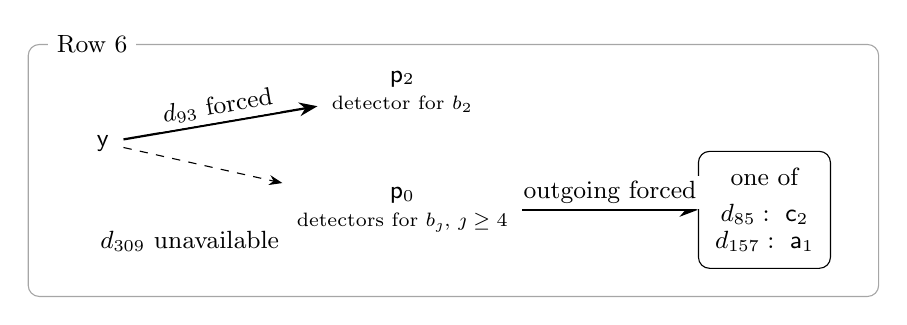
\begin{tikzpicture}[
  >=Stealth,
  every node/.style={font=\small},
  entry/.style={inner sep=5pt},
  arrowlabel/.style={fill=white,inner sep=2pt,align=center}
]
  \draw[rounded corners,black!35] (-0.55,-1.95) rectangle (10.25,1.25);
  \node[anchor=west,fill=white,inner sep=3pt] at (-0.3,1.25)
    {Row $6$};
  \node[entry] (y) at (0.4,0) {$\mathsf y$};
  \node[entry,align=center] (p2) at (4.2,0.65)
    {$\mathsf p_2$\\[-1pt]\scriptsize detector for $b_2$};
  \node[entry,align=center] (p0) at (4.2,-0.85)
    {$\mathsf p_0$\\[-1pt]\scriptsize detectors for $b_{\jmath}$, $\jmath\ge4$};
  \node[draw,rounded corners,align=center,inner sep=6pt] (out) at (8.8,-0.85)
    {one of\\[2pt]
     $d_{85}:\ \mathsf c_2$\\[-1pt]
     $d_{157}:\ \mathsf a_1$};
  \draw[->,thick] (y) -- node[arrowlabel,above,sloped]
    {$d_{93}$ forced} (p2);
  \draw[->,dashed] (y) -- (p0);
  \node[arrowlabel] at (1.5,-1.25) {$d_{309}$ unavailable};
  \draw[->,thick] (p0) -- node[arrowlabel,above]
    {outgoing forced} (out);
\end{tikzpicture}
\caption{The final constraint in row $6$.  The known survivor $b_2$
forces the $d_{93}$ pairing, so its source $\mathsf y$ cannot also
hit $\mathsf p_0$ at length $309$.  The possible $\mathsf x$ incoming
at length $273$ lies in row $3$.  Thus $\mathsf p_0$ must support
one of the two indicated outgoing differentials; the argument does
not choose between them.  The diagram records logical constraints,
not chronological order: length $85$ precedes length $93$.}
\label{g:forcing-figure}
\end{figure}


The $\mathsf p_0$ offset $(6,34)$ has key
$6-3\cdot34=3$ modulo nine.  In row $6$ it
therefore has total key zero.  Every
detector with $\jmath\ge4$ in
\eqref{g:detector-coordinates} has
\[
 t\equiv0\pmod3,\qquad
 t-3u=-40\cdot3^{\jmath-2}\equiv0\pmod9.
\]
It is exactly a $\mathsf p_0$ copy of this
key.  The unit translations of
Proposition~\ref{g:unit313} identify all such
copies through the relevant pages.  In
particular none can be an earlier incoming
Tate boundary, and each must have the forced
outgoing just proved.  This contradicts the
cycle property of the image of any surviving
sphere class.  Hence no $b_{\jmath}$ with
$\jmath\ge4$ survives.

For comparison, the $\jmath=3$ detector has
key $6$, whereas the $\jmath=2$ detector has
key $5$.  Thus the tail exclusion does not
decide $b_3$ by the same argument.  Its
survival and order-three representative
will be constructed separately in
Section~\ref{sec:cube}.
\end{proof}

\section{An order-three element in the 322-stem}
\label{sec:cube}

This section constructs the remaining positive class.  The construction is
independent of the height-six detector.  Its geometric input is the known
order-three Kervaire element in the 106-stem; its algebraic input is
Lemma~\ref{finite:main}, proved in Section~\ref{sec:finite}.  A truncated
extended cube first gives a map into a four-cell spectrum \(T\) containing
the Moore spectrum \(M=S/3\), with quotient \(\Sigma^4M\).  We construct
a map of Adams--Novikov filtration at least two with the same image in
that quotient; subtracting it gives a map that lifts to \(M\).  Keeping
track of that correction is essential both for the primary Steenrod
operation and for the additive order of the resulting sphere element.
Extended powers have long connected primary operations with unstable
and stable homotopy; see Toda~\cite{TodaExtended} and
May~\cite[Sections~2--3]{MayOperations}.
The construction below specifies the finite lens-space truncation
and the two Moore-spectrum corrections needed in this dimension.

\begin{theorem}\label{cube:order-three}
There is an element \(\theta\in\pi_{322}S_{(3)}\) detected by \(b_3\) in the
mod-three Adams spectral sequence such that \(3\theta=0\).
In particular, \(\theta\) has additive order exactly three.
\end{theorem}

\subsection{The strong criterion and the filtration conventions}

All spectra and maps in this section are localized at three.  Write \(S\)
for the localized sphere and let
\begin{equation}\label{cube:moore-triangle}
 S\xrightarrow{3}S\xrightarrow{i}M\xrightarrow{q}\Sigma S
\end{equation}
be the Moore cofibre sequence.  A power of a sphere class always denotes
its product in the stable homotopy ring of \(S\).

We use the following established form of the strong odd-primary Kervaire
criterion.  Our statement includes the change of indices and the duality
that will be needed below.

\begin{lemma}[Strong Kervaire criterion]\label{cube:strong-criterion}
Let \(j\geq0\) and \(m=3^{j+1}\).  The following conditions are equivalent:
\begin{enumerate}[label=\textup{(\roman*)}]
\item The detection coset of \(b_j\) contains an element of additive order
three in \(\pi_{4m-2}S\).
\item There is a stable map
\[
 \Sigma^{4m-2}M=P^{4m-1}(3)\longrightarrow S
\]
whose cone has nonzero reduced power \(\mathcal P^m\).
\item There is a stable map \(a:S^{4m-1}\to M\) for which
\[
 \mathcal P^m:H^0(C_a;\F_3)\longrightarrow H^{4m}(C_a;\F_3)
\]
is nonzero.
\end{enumerate}
In condition \textup{(iii)}, if \(qa=\Sigma\vartheta\), then
\(3\vartheta=0\) in actual sphere homotopy.  The strong criterion identifies
\(\vartheta\), up to the usual nonzero scalar normalization, as a nonzero
class detected by \(b_j\).
\end{lemma}

\begin{proof}
The equivalence of the first two conditions is Selick's strong
odd-primary criterion, in its stable Moore-space formulation
\cite[Theorems~1.1 and~3.3]{Selick}; see also the proof of
\cite[Theorem~1.1]{Amelotte}.  In the notation of that formulation the
stem is \(2m(p-1)-2\), and the detecting Adams class is \(b_{k-1}\) when
\(m=p^k\).  Thus at \(p=3\) and \(k=j+1\) the stem is \(4m-2\) and the
class is precisely \(b_j\).

For completeness, Spanier--Whitehead duality gives the last equivalence
without changing the primary test.  If
\(g:\Sigma^{4m-2}M\to S\), then \(DM\simeq\Sigma^{-1}M\) and
\[
 a=\Sigma^{4m-1}Dg:S^{4m-1}\longrightarrow M,\qquad
 C_a\simeq\Sigma^{4m}DC_g.
\]
The cohomology degrees of \(C_g\) and \(C_a\) are, respectively,
\(\{0,4m-1,4m\}\) and \(\{0,1,4m\}\).  Conjugation in the Steenrod
algebra sends \(\mathcal P^m\) to \(-\mathcal P^m\) modulo products of
positive reduced powers
\cite[Section~7, pp.~166--167]{Milnor}.  Such products vanish on the two cones,
because the necessary intermediate degrees are absent.  Consequently
duality preserves nonvanishing of the indicated operation.
Finally, \(3\vartheta=0\) follows directly from
\eqref{cube:moore-triangle}; the detection and nonvanishing are part of
the strong criterion.  Thus the criterion concerns an actual
order-three representative, rather than an order assertion about an
associated-graded group.
\end{proof}

Put
\[
 I=\operatorname{fib}(S\longrightarrow\BP),\qquad
 F_fZ=I^{\wedge f}\wedge Z,\qquad
 L_fZ=F_fZ/F_{f+1}Z.
\]
The Adams--Novikov filtration of a homotopy group is
\[
 F^f\pi_kZ=\im\bigl(\pi_kF_fZ\longrightarrow\pi_kZ\bigr).
\]
We retain the usual indices
\[
 E_r^{f,t}(Z)\Longrightarrow\pi_{t-f}Z,\qquad
 d_r:E_r^{f,t}(Z)\longrightarrow E_r^{f+r,t+r-1}(Z).
\]
In particular \(L_fS\simeq\BP\wedge I^{\wedge f}\).  Flatness of
\(\BP_*\BP\) identifies its homotopy groups with the desuspended
normalized cobar terms: they are torsion-free and supported in degrees
\(-f\bmod4\).  The groups for \(L_fM\) are their reductions modulo three.
It follows that
\begin{equation}\label{cube:sparseness}
 E_r^{f,t}(M)=0\quad\text{unless }t\equiv0\pmod4,
 \qquad E_2(M)=E_5(M),\quad E_6(M)=E_9(M).
\end{equation}
The tower description and its multiplicative pairings agree with the
usual Adams--Novikov spectral sequence; the unit-cube comparison and
the pairing conventions are recalled in Lemma~\ref{finite:pairing}.
The orientation \(\BP\to\HF\) gives the comparison with the ordinary
mod-three Adams tower.

These filtrations are finite in each fixed stem of a bounded-below
spectrum.  Indeed \(I\) is at least 3-connective: the unit is an
isomorphism on \(\pi_0\), and the localized sphere has no homotopy in
degrees one and two.  The connectivity of \(F_fZ\) therefore tends to
infinity with \(f\).  We shall use this finiteness when passing from
vanishing associated-graded groups to vanishing homotopy classes.

We also recall explicitly the elementary property of the first Adams
invariant that is used to control the corrections.

\begin{lemma}\label{cube:primary-invariant}
For a map \(u:A\to B\) inducing zero in mod-three homology, the short
exact sequence of Steenrod comodules
\[
 0\longrightarrow H_*B\longrightarrow H_*C_u
   \longrightarrow \Sigma H_*A\longrightarrow0
\]
is its ordinary Adams filtration-one invariant.  This invariant is
natural and additive in \(u\).  It vanishes for a composite of two maps
that induce zero in mod-three homology, and hence for a map of
Adams--Novikov filtration at least two.
\end{lemma}

\begin{proof}
The first Adams obstruction measures whether the displayed comodule
extension splits.  Cone maps give its naturality.  To add two maps,
first take their direct sum and then use the diagonal on the source
and the fold on the target; the corresponding pullback and pushout of
extensions give their Baer sum.  If \(u=vw\) and both \(v_*\) and
\(w_*\) vanish, the cone comparison from \(w\) to \(vw\) identifies
the extension of \(vw\) with the pushout of the extension of \(w\)
along \(v_*=0\).  This pushout is split.

The maps between two successive stages of the mod-three Adams tower
are homology-zero maps.  Thus a factorization through its second stage
has zero invariant.  The comparison \(\BP\to\HF\) supplies this
factorization for a map of Adams--Novikov filtration at least two.
\end{proof}

Whenever the cone has no ambiguity in the bottom and tested top
degrees, the coefficient of a primary reduced power between those
degrees is a component of this extension invariant.  In particular,
subtracting a map as in the last assertion of
Lemma~\ref{cube:primary-invariant} does not change that coefficient.

\subsection{A filtration-ten cube}

Set
\begin{equation}\label{cube:dimensions}
 t=108,\qquad n=t-1=107,\qquad N=3t-2=322.
\end{equation}
The classical Kervaire detection coset in \(\pi_{106}S\) contains
an element of order three detected by
\(b_2\); see \cite[Corollary~1.2 and its proof]{Amelotte} and
\cite[Table~A3.4]{Ravenel}.  By
Lemma~\ref{cube:strong-criterion}, choose
\[
 a_0:S^n\longrightarrow M
\]
with nonzero \(\mathcal P^{27}\) from the bottom to the top of its cone,
and write \(qa_0=\Sigma x\), where \(x\in\pi_{106}S\).

\begin{proposition}\label{cube:cubic-filtration}
The reduction of the cube satisfies
\[
 ix^3\in F^{10}\pi_{318}M.
\]
\end{proposition}

\begin{proof}
The class of \(a_0\) has Adams--Novikov filtration one.  Filtration
zero is excluded by the support of \(\pi_*\BP M\), while filtration
at least two is excluded by its nonzero primary test and
Lemma~\ref{cube:primary-invariant}.  Let
\[
 z\in E_2^{1,108}(M)
\]
be its permanent leading class.

We use the notation of Section~\ref{sec:finite}: \(v=v_1\),
\(a=[t_1]\), \(B\) is the reduced integral 3-Bockstein, and
\begin{align*}
 y&=\frac{\eta_R(v_2^9-v_1^8v_2^7)-(v_2^9-v_1^8v_2^7)}{v_1^9},\\
 t_7'&=\frac{\eta_R(v_2^7)-v_2^7}{v_1}
 \qquad\text{in the mod-three cobar complex}.
\end{align*}
By the unconditional basis calculation \eqref{finite:low-classes}, write
\[
 z=\lambda y+\nu t'_7+\mu v^{26}a,
 \qquad \lambda,\nu,\mu\in\F_3.
\]
After setting all positive coefficient generators \(v_i\) to zero,
these representatives specialize to \(\lambda t_1^{27}\).
Every one-cobar boundary also specializes to zero, since the
positive coefficient ideal is invariant.  The Thom comparison
sends \(t_1\), up to a unit, to the first reduced-power dual
generator; its conjugate Milnor convention changes only this
unit.  Hence \(\lambda\), up to a unit, is the
\(\mathcal P^{27}\) coefficient of \(C_{a_0}\), and is nonzero.
Rescale \(a_0\) to make \(\lambda=1\).
Lemma~\ref{finite:main} then gives
\begin{equation}\label{cube:leading-class}
 z=y+\mu v^{26}a,\quad\mu\in\F_3,\qquad B(y)^3=0.
\end{equation}

The boundary along \(q\) increases Adams--Novikov filtration by one
and induces the integral 3-Bockstein; this is the geometric boundary
theorem \cite[Theorem~2.3.4]{Ravenel}.  Here it can be seen directly
on two layers.  Put \(X=F_2S\), \(Y=F_1S\), and \(Z=Y/X\).
A lift of \(a_0\) to \(Y/3\) and an integral lift to \(Z\) of its
image in \(Z/3\) give a class in
\[
 Q=(Y/3)\mathbin{\times}_{Z/3}Z.
\]
The integral lift exists because the homotopy of \(Z\) is
torsion-free.  Comparing fibres over \(Z\) yields the triangle
\[
 X\xrightarrow{\,3\iota\,}Y
 \longrightarrow Q\longrightarrow\Sigma X,
\]
where \(\iota:X\to Y\) is the inclusion: the fibre of
\(Y\to Q\) identifies with the fibre of \(X\to X/3\),
and its map into \(Y\) is \(3\iota\).
Projection to \(Y/3\) identifies the resulting boundary with a lift
of \(x\) to \(F_2S\).  Projection to \(Z\) says that three times its
layer symbol is the \(d_1\) of the chosen integral lift.  Division
by three in the torsion-free layer gives exactly the stated
Bockstein, with a harmless convention-dependent sign.

After reducing again by \(i\), the filtration-two symbol is
\(\pm B(z)=\pm B(y)\).  Indeed the Bockstein is a derivation,
\[
 B(v)=\pm a,\qquad B(a)=0,\qquad a^2=0,
\]
so \(B(v^{26}a)=0\).  Multiplicativity of the sphere tower and its
pairing with the Moore tower puts \(ix^3\) in filtration at least
six, with filtration-six symbol represented by \(\pm B(y)^3\).
This symbol is zero by \eqref{cube:leading-class}.  Thus \(ix^3\)
has filtration greater than six.  Its stem is \(318\equiv2\bmod4\),
so \eqref{cube:sparseness} makes ten the next possible filtration.
\end{proof}

\subsection{The truncated extended cube}

Write \(\Sigma_3=C_3\rtimes C_2\), where the generator of \(C_2\)
acts on \(C_3\) by inversion.  Let \(\rho\) be the real permutation
representation on three letters and write
\[
 \rho=\mathbf1\oplus\lambda.
\]
Here \(\lambda\) is a real two-plane.  Restricted to \(C_3\) it is
the faithful complex character, while \(C_2\) acts by conjugation;
in particular its orientation character is \(\mathrm{sgn}\).

Let \(L^{(2)}=S^1\cup_3D^2\) be the two-skeleton of a lens-space
model for \(BC_3\).  A useful explicit cover is the subspace
\[
 \widetilde L^{(2)}
 =\{(z_1,z_2)\in S(\C^2):
       z_2\in\bigcup_{\zeta^3=1}\zeta\mathbf R_{\geq0}\}.
\]
Scalar multiplication by a third root of unity and complex
conjugation give the required \(C_3\rtimes C_2\)-action.  This
cover consists of three disks with their boundary circles
identified.  The \(C_3\)-quotient is \(L^{(2)}\), with its
degree-three attachment.

Take a free contractible \(C_2\)-space \(EC_2\), let \(C_3\) act
trivially on this extra factor, and put
\[
 \mathcal B=(L^{(2)})_{hC_2},\qquad
 \mathcal P=\widetilde L^{(2)}\times EC_2.
\]
Thus \(\mathcal P\to\mathcal B\) is a principal \(\Sigma_3\)-bundle.
A classifying map to \(B\Sigma_3\) gives a natural comparison
between
\begin{equation}\label{cube:truncated-functor}
 D^\circ(X)=\mathcal P_+\wedge_{\Sigma_3}X^{\wedge3},
 \qquad
 D_3(X)=E\Sigma_{3+}\wedge_{\Sigma_3}X^{\wedge3}.
\end{equation}
The permutation of smash factors is the usual permutation action
in spectra, including its signs on odd-dimensional spheres.

\begin{lemma}\label{cube:lens-thom}
The base \(\mathcal B\) has cohomological dimension at most two
for 3-local local coefficient systems, and
\[
 \widetilde H^*(\mathcal B;A)=0
\]
for every constant 3-local abelian group \(A\).
Moreover,
\begin{equation}\label{cube:thom-identifications}
 D^\circ(S^1)\simeq\Sigma^4M,\qquad
 D^\circ(S^n)\simeq\Sigma^NM.
\end{equation}
These identifications can be chosen so that
\begin{equation}\label{cube:quotient-cube}
 D^\circ(qa_0)=x^3 1_M:
       \Sigma^NM\longrightarrow\Sigma^4M.
\end{equation}
\end{lemma}

\begin{proof}
Since two is invertible, the spectral sequence for the homotopy
orbits by \(C_2\) takes invariants exactly.  The cellular complex
of \(L^{(2)}\) has dimension two, proving the assertion about
local coefficients.  With constant coefficients its possible
reduced cohomology groups are
\(\ker(3:A\to A)\) in degree one and \(A/3A\) in degree two.
Inversion acts by minus one on both, so neither has nonzero
\(C_2\)-invariants.  In particular the augmentation
\(\Sigma^\infty\mathcal B_+\to S\) is a 3-local equivalence:
its cofibre is bounded below and has zero integral localized
homology, hence is zero by the stable Hurewicz theorem.

The Thom spectrum of \(\rho\) over \(\mathcal B\) is
\(D^\circ(S^1)\).  Its orientation system is \(\mathrm{sgn}\).
On the lens skeleton, integral reduced homology is
\(\Z/3\) in degree one, and inversion acts by minus one.
Twisting by \(\mathrm{sgn}\) therefore retains that group
and removes the degree-zero group.  The Thom homology is
consequently just \(\Z/3\) in degree four.
To identify the spectrum, realize its lowest homotopy generator
by \(S^4\); it has order three by the lowest-degree Hurewicz
isomorphism and extends to \(\Sigma^4M\).
The extension is an integral homology equivalence and therefore
a 3-local equivalence of bounded-below spectra.

The difference bundle \((n-1)\rho\) is oriented, since \(n-1=106\)
is even, and is stably spherically trivial after localization at
three.  Indeed its spherical classifying map lifts to the
classifying space of degree-one stable sphere equivalences.
This space is simply connected and its second homotopy group
is \(\pi_1S_{(3)}=0\).  The subsequent Postnikov obstructions
vanish by the cohomological dimension of \(\mathcal B\).
There is no inverse-limit ambiguity: for a fixed homotopy
degree of the mapping space, the fibres of its Postnikov
tower have zero homotopy in that degree once their
Eilenberg--Mac Lane degree exceeds it by more than two.
Thus the required compatible nullhomotopies exist.
Trivializing this difference bundle identifies
\[
 D^\circ(S^n)\simeq
 \Sigma^{3(n-1)}D^\circ(S^1)
 \simeq\Sigma^{3n+1}M=\Sigma^NM.
\]

Before taking Thom spectra, \(D^\circ(qa_0)\) is a map
from the sphere bundle \(S^{n\rho}\) to \(S^\rho\).
After the difference bundle is trivialized, its fibrewise
mapping spectrum is the constant spectrum
\(S^{-3(n-1)}\): endomorphisms of the remaining invertible
sphere line identify canonically with scalars.
Sections of this constant spectrum are determined, on
homotopy classes, by evaluation at one point, because
\(\Sigma^\infty\mathcal B_+\simeq S\).
At that point the map is the ordinary smash cube of \(qa_0\),
namely the suspension of \(x^3\) in the indicated degrees.
This proves \eqref{cube:quotient-cube}, up to a 3-local unit
which is absorbed in the source identification.
\end{proof}

The same base calculation supplies the nonzero Euler pairing
that will detect a primary reduced power.  Namely
\begin{equation}\label{cube:euler-pairing}
 e(\lambda)\frown-:
 H_2(\mathcal B;\F_3^{\mathrm{sgn}})
 \longrightarrow H_0(\mathcal B;\F_3)
\end{equation}
is nonzero.  On restricting to the lens skeleton, \(e(\lambda)\)
is the mod-three first Chern class of the faithful \(C_3\)-line.
It is the nonzero Bockstein of a fundamental-group character.
Its evaluation on the mod-three two-cell is a unit.  The
orientation twist cancels the inversion sign, so taking
\(C_2\)-invariants preserves this pairing.

\begin{lemma}\label{cube:attachment}
There is a triangle
\begin{equation}\label{cube:T-triangle}
 \Sigma^3M\xrightarrow{g}M\xrightarrow{j_T}T
      \xrightarrow{\pi_T}\Sigma^4M
\end{equation}
and a map \(F:\Sigma^NM\to T\) such that
\[
 \pi_TF=x^3 1_M.
\]
Both \(j_T\) and the natural map \(D^\circ M\to T\) are
isomorphisms on bottom mod-three homology.
\end{lemma}

\begin{proof}
Filter \(D_3M\) by the number of upper Moore cells in its
three input factors.  The four successive layers, before
simplification, have stabilizers
\(\Sigma_{3-r}\times\Sigma_r\), \(0\leq r\leq3\).
The bottom layer is \(\Sigma^\infty B\Sigma_{3+}\).
For one upper cell, the \(\Sigma_2\)-stabilizer acts trivially
on its one-dimensional sphere; the layer is therefore
\(\Sigma S\) after localization at three.  For two upper
cells, interchanging the two odd spheres is the sign action.
Its \(\Sigma_2\)-homotopy orbits are zero at three, so this
layer disappears.  The top layer is \(D_3S^1\).

The attachment of the one-cell layer to the bottom is degree
three.  One can compute it in the cellular complex of
\(M^{\wedge3}\): a chosen one-upper-cell generator has
boundary three times the bottom generator.
Passing to \(\Sigma_3\)-coinvariants identifies the three
choices of this generator; it does not add their three
boundaries.  Thus the attachment has degree three, not nine.
Since the reduced suspension spectrum of the connected
space \(B\Sigma_3\) has zero \(\pi_0\), this attachment has
no reduced component.

It follows that the part \(K\) below the top layer has a
projection \(r:K\to M\) inducing an isomorphism on bottom
homology; explicitly, \(K\) is the cofibre of the bottom
degree-three map into \(\Sigma^\infty B\Sigma_{3+}\), and
the augmentation gives \(r\).
Pull back \(D_3M\to D_3S^1\) along
\(D^\circ S^1\to D_3S^1\), obtaining \(U\), and push out
its fibre along \(r\).  These constructions give a diagram
of triangles
\[
\begin{tikzcd}[column sep=large]
 K \arrow[r] \arrow[d,"r"'] &
 U \arrow[r] \arrow[d] &
 D^\circ S^1 \arrow[d,equal] \arrow[r] &
 \Sigma K \arrow[d,"\Sigma r"]\\
 M \arrow[r,"j_T"'] &
 T \arrow[r,"\pi_T"'] &
 D^\circ S^1 \arrow[r] &
 \Sigma M .
\end{tikzcd}
\]
Use \eqref{cube:thom-identifications} in the lower row
and desuspend its boundary to define \(g\).
The natural comparison square for \(D^\circ q\) gives
\(D^\circ M\to U\to T\); composing it with
\(D^\circ a_0\) gives \(F\).
Its quotient is \eqref{cube:quotient-cube}.
The bottom-homology claims follow because the comparisons
of base orbits preserve \(H_0\), the projection \(r\)
preserves the bottom generator, and the remaining quotient
\(\Sigma^4M\) has no homology near degree zero.
\end{proof}

\begin{proposition}\label{cube:primary-detection}
The cone of \(F:\Sigma^NM\to T\) has a nonzero operation
\[
 \mathcal P^{81}:H^0(C_F;\F_3)\longrightarrow
 H^{N+2}(C_F;\F_3).
\]
\end{proposition}

\begin{proof}
Throughout this proof homology has coefficients \(\F_3\).
We adapt Toda's diagonal cone construction
\cite[Section~1, Theorem~2]{TodaExtended} to the truncated functor
\(D^\circ\). Applying the diagonal cone nullhomotopy gives a natural map
\[
 C_{D^\circ a_0}\longrightarrow D^\circ(C_{a_0}).
\]
Compose it with the map \(D^\circ C_{a_0}\to D^\circ S^t\)
induced by \(C_{a_0}\to S^t\).  This composite is zero on
\(D^\circ M\), and therefore factors through
\(C_{D^\circ a_0}/D^\circ M\simeq\Sigma D^\circ S^n\).
The resulting map
\begin{equation}\label{cube:diagonal-thom}
 \Sigma D^\circ S^n\longrightarrow D^\circ S^t
\end{equation}
comes from the diagonal trivial line in the permutation
representation.  More explicitly, use the same interval
parameter in the three cone factors and then collapse
their ends.  Its normal representation is
\(\rho-\mathbf1=\lambda\).  The resulting Thom map is
therefore the Euler map for \(\lambda\).
Since \(N+2=3t=324\), the map on the tested top homology
is precisely the cap product \eqref{cube:euler-pairing};
it is nonzero.

The spectrum \(D^\circ M\) has homology only in degrees
at most five: its fibre \(M^{\wedge3}\) has homology in
degrees zero through three and its base has homological
dimension two.  Consequently the suspended top class
of \(D^\circ S^n\simeq\Sigma^NM\) gives a class
\(c\in H_{3t}(C_{D^\circ a_0})\).
Let \(u\in H_t(C_{a_0})\) be the top generator.
In the homology spectral sequence over \(\mathcal B\),
the fibre of \(D^\circ C_{a_0}\) has tensor-product
homology with degrees chosen from \(\{0,1,t\}\).
In total degree \(3t\), the sole possible term is
\[
 H_0\bigl(\mathcal B;\F_3\{u^{\otimes3}\}\bigr);
\]
the action is trivial since \(t\) is even.
There is no possible differential into or out of this
term, nor another term in its total degree.
Projection to \(D^\circ S^t\) identifies it with the
fibre generator there.  By \eqref{cube:diagonal-thom},
the image of \(c\) is a nonzero multiple of
\(u^{\otimes3}\).

The bottom fibre class survives as well.  The Cartan formula
for reduced powers \cite[Section~2, Property~2.5]{Milnor} on the
fibre gives
\[
 \mathcal P_*^{81}(u^{\otimes3})
       =(\mathcal P_*^{27}u)^{\otimes3}\ne0.
\]
Indeed, to reach degree zero each tensor factor must
be lowered from degree \(t=108\) by \(\mathcal P_*^{27}\);
all other Cartan terms have zero contribution to the
bottom.  Naturality shows that
\(\mathcal P_*^{81}c\) is nonzero in
\(H_0(C_{D^\circ a_0})\).

Finally, the map \(D^\circ M\to T\) and the identity on
the source induce \(C_{D^\circ a_0}\to C_F\).
It is an isomorphism on the bottom and on the tested top
homology.  Applying naturality again proves the assertion.
\end{proof}

\subsection{Endomorphisms and the two obstruction components}

\begin{lemma}\label{cube:endomorphisms}
There is a unital multiplication \(\mu:M\wedge M\to M\),
and evaluation on the bottom cell admits a splitting
\begin{equation}\label{cube:end-splitting}
 \mathcal E=F(M,M)\simeq M\vee\Sigma^{-1}M.
\end{equation}
Write \(\varepsilon:\mathcal E\to M\) for evaluation,
\(s:M\to\mathcal E\) for its section, and
\(\tau:\mathcal E\to\Sigma^{-1}M\) for the other projection.
The second summand includes by precomposition with
\(q:M\to\Sigma S\), and \(s(i)=1_M\).
No associativity of \(\mu\) is required.
\end{lemma}

\begin{proof}
The Moore sequence gives \(\pi_1M=0\) and
\(\pi_0M=\F_3\).  Applying \([-,M]\) to that sequence
shows that restriction to the bottom identifies
\([M,M]\) with \(\pi_0M\).  In particular \(3\,1_M=0\).
The cofibre sequence
\[
 M\xrightarrow{3}M\longrightarrow M\wedge M
\]
then allows the identity of \(M\) to extend to a
multiplication \(\mu\) with one unit law.  The other
unit composite has the same bottom restriction as
the identity, so it is the identity by the same
restriction calculation.

Applying \(F(-,M)\) to \eqref{cube:moore-triangle}
identifies the fibre of
\(\varepsilon:F(M,M)\to F(S,M)=M\) with
\(F(\Sigma S,M)=\Sigma^{-1}M\).
Adjunction applied to \(\mu\) gives the section \(s\).
Its value on \(i\) is the identity by the unit law.
Splitting this fibre sequence proves the assertions.
\end{proof}

The correction will be made inside \(F_2T\).  It is
important to distinguish its tower from the full
Adams--Novikov tower.

\begin{lemma}\label{cube:relative-tower}
Let \(\widetilde E_r\) be the spectral sequence of
\[
 \cdots\longrightarrow F_4M\longrightarrow F_3M
       \longrightarrow F_2M,
\]
with absolute filtration indices retained.  Its
comparison \(c_r:\widetilde E_r^{f,t}\to E_r^{f,t}(M)\)
has the following properties:
\[
\begin{array}{c|c|c}
\text{page}&\text{surjective}&\text{isomorphic}\\ \hline
5&f\geq2&f>2\\
6=9&f\geq2&f\geq7\\
10&f\geq2&f\geq11.
\end{array}
\]
These assertions hold also for maps induced by fixed
endomorphisms of \(M\), with their appropriate degree
shifts.
\end{lemma}

\begin{proof}
The layer complex agrees with the full \(E_1\)-complex
above filtration two.  In filtration two it has the
same cycles but omits incoming \(d_1\)-boundaries.
This gives the stated comparison on \(E_2\), hence on
\(E_5\) by sparseness.

For clarity, a full \(d_r\)-cycle lifts to a cycle
whenever comparison is surjective in its slot and
injective in its outgoing slot: the differential of
any lift maps to zero and must therefore vanish.
Comparison on the resulting homology is injective
as well if it is injective in the current slot and
surjective in the incoming slot, because a full
boundary can then be lifted.

Apply this first to \(d_5\).  An outgoing slot from
filtration \(f\geq2\) has filtration at least seven,
where \(c_5\) is an isomorphism.  Thus \(c_6\) is
surjective for every \(f\geq2\).  If \(f\geq7\), the
incoming slot has filtration \(f-5\geq2\), so the
same argument gives an isomorphism.  Sparseness
identifies this page with \(E_9\).
For \(d_9\), all outgoing slots again compare
isomorphically.  When \(f\geq11\), the incoming
filtration \(f-9\) is at least two, proving the
last row.  Everything is natural in maps of the
underlying tower.
\end{proof}

Write the filtration of the abutment of this restricted
tower as
\[
 \mathcal F^f\pi_kF_2M
   =\im\bigl(\pi_kF_fM\longrightarrow\pi_kF_2M\bigr),
 \qquad f\geq2.
\]
It is finite by connectivity, just as the full filtration.

\begin{proposition}\label{cube:correction}
There is a map \(F':\Sigma^NM\to F_2T\) whose composite
to \(T\) has the same quotient under \(\pi_T\) as \(F\).
\end{proposition}

\begin{proof}
Choose a lift
\(\widehat c\in\pi_{318}F_{10}M\) of \(ix^3\) using
Proposition~\ref{cube:cubic-filtration}, and let \(c\)
be its image in \(\pi_{318}F_2M\).  Smash the section
in Lemma~\ref{cube:endomorphisms} with \(I^{\wedge2}\)
and put
\[
 w=s_*(c)\in\pi_{318}F_2\mathcal E.
\]
After forgetting filtration, \(w\) is exactly
\(x^3 1_M\), because \(s(i)=1_M\).

Postcomposition with \(g:\Sigma^3M\to M\) defines
\[
 \gamma:\Sigma^3\mathcal E\longrightarrow\mathcal E.
\]
The obstruction to lifting \(w\) through the triangle
\eqref{cube:T-triangle} smashed with \(I^{\wedge2}\)
is
\[
 \gamma_*(w)\in\pi_{321}F_2\mathcal E.
\]
We show separately that both components of this
obstruction under \eqref{cube:end-splitting} vanish.

\emph{The first component.}
Forgetting filtration makes the whole obstruction
zero, since \(F\) is already an actual lift of
\(x^3 1_M\).  Its first component lies in
\(\pi_{321}F_2M\), and the map
\[
 \pi_{321}F_2M\longrightarrow\pi_{321}M
\]
is injective.  To see this, the quotient \(M/F_2M\)
has its two layers \(L_0M\) and \(L_1M\), both with
zero \(\pi_{322}\): their support degrees are,
respectively, \(0\) and \(3\) modulo four, whereas
\(322\equiv2\).  Thus \(\pi_{322}(M/F_2M)=0\), and
the long exact sequence gives the injection.
The first component is therefore zero already in
the restricted tower.

\emph{The second component.}
The fixed composite
\[
 \Sigma^3M\xrightarrow{\Sigma^3s}\Sigma^3\mathcal E
     \xrightarrow{\gamma}\mathcal E
     \xrightarrow{\tau}\Sigma^{-1}M
\]
suspends to a map \(h:\Sigma^4M\to M\).
Under the splitting, the second obstruction is
precisely \(h_*(c)\in\pi_{322}F_2M\).
The map \(h\) on \(\BP_*\)-homology is multiplication
by a scalar multiple of \(v_1\), since a
\(\BP_*\)-linear degree-four map
\(\BP_*M\to\BP_*M\) is determined by its value in
\(\BP_4M=\F_3\{v_1\}\).
This is a comodule map: \(v_1\) is primitive modulo three,
by \(\eta_R(v_1)=v_1+3t_1\).
Functoriality of the normalized cobar complex therefore
identifies \(E_2(h)\) with that literal coefficient
multiplication.  The map of Adams towers passes this
identification to \(E_5\) and \(E_6\); the coefficient
\(v_1\) is permanent by the target-vanishing argument in
Section~\ref{sec:finite}.
No multiplicativity assumption on \(h\) is used.
Its action on the full \(E_6\)-page in the
relevant slots is consequently a scalar multiple of
\begin{equation}\label{cube:v-obstruction}
 v_1:E_6^{10,328}(M)\longrightarrow E_6^{10,332}(M),
\end{equation}
which is zero by Lemma~\ref{finite:main}.
Lemma~\ref{cube:relative-tower} is an isomorphism on
both these \(E_6\)-slots.  Consequently \(h\) induces
zero on the filtration-ten associated-graded map
of the restricted abutment.  Since
\(c\in\mathcal F^{10}\pi_{318}F_2M\), this proves
\[
 h_*(c)\in\mathcal F^{11}\pi_{322}F_2M
          =\mathcal F^{14}\pi_{322}F_2M.
\]
The equality follows from sparseness: in stem 322
only filtrations congruent to two modulo four can
occur.

For every such filtration \(f\geq14\),
Lemma~\ref{finite:main}, including its high-filtration
estimate, gives
\[
 E_{10}^{f,322+f}(M)=0.
\]
The comparison of Lemma~\ref{cube:relative-tower}
is an isomorphism there, so the restricted
\(E_{10}\)-groups vanish as well.  Every
associated-graded quotient of
\(\mathcal F^{14}\pi_{322}F_2M\) is therefore zero.
Increasing connectivity makes this filtration
finite, and hence
\(\mathcal F^{14}\pi_{322}F_2M=0\).
This proves that the second component vanishes.

Notice why the two page arguments were separated:
an incoming full \(d_9\) at filtration ten may
start in filtration one, which the restricted
tower omits.  No \(E_{10}\)-comparison in
filtration ten was asserted or used.  The zero
map \eqref{cube:v-obstruction} removes that
filtration on \(E_6\) before the higher
\(E_{10}\)-vanishing is applied.

We have now proved \(\gamma_*(w)=0\).
The triangle \eqref{cube:T-triangle} smashed with
\(I^{\wedge2}\) supplies the desired lift.
More explicitly, \(M\) is dualizable, so
\[
 F(M,I^{\wedge2}\wedge Z)
   \simeq I^{\wedge2}\wedge F(M,Z).
 \]
The exact sequence obtained by applying \(F(M,-)\)
to that triangle therefore identifies the
vanishing obstruction just calculated with the
existence of \(F':\Sigma^NM\to F_2T\).
Its quotient represents \(w\), whose underlying
map is \(x^3 1_M=\pi_TF\).
\end{proof}

\subsection{The sphere element and its order}

\begin{proof}[Proof of Theorem~\ref{cube:order-three}]
Let \(\overline F'\) be the composite of the map in
Proposition~\ref{cube:correction} with \(F_2T\to T\).
Its quotient equals that of \(F\), so the difference
has a lift
\[
 Z:\Sigma^NM\longrightarrow M,\qquad
 j_TZ=F-\overline F'.
\]
The map \(\overline F'\) has Adams--Novikov filtration
at least two.  The maps \(F\), \(\overline F'\), and
\(F-\overline F'\) induce zero on mod-three homology for degree reasons, so
Lemma~\ref{cube:primary-invariant} and additivity
show that the primary invariant of
\(F-\overline F'\) equals that of \(F\).
Since \(j_T\) is an isomorphism on bottom homology,
the cone comparison from \(Z\) to \(j_TZ\) is an
isomorphism on the bottom and on the tested top
degrees.  Proposition~\ref{cube:primary-detection}
thus gives a nonzero
\[
 \mathcal P^{81}:H^0(C_Z;\F_3)\longrightarrow
                      H^{324}(C_Z;\F_3).
\]

Use the splitting of Lemma~\ref{cube:endomorphisms}
to write the class of \(Z\) as the sum of its
section component and its quotient-precomposition
component.  The section component is \(s_*(z_0)\)
for some \(z_0\in\pi_NM=\pi_{322}M\).
This class has Adams--Novikov filtration at
least two: the degree-322 homotopy of both
\(L_0M\) and \(L_1M\) is zero, so it lifts
successively through \(F_1M\) and \(F_2M\).
Applying the section to that lift shows that
the corresponding map \(\Sigma^NM\to M\)
also factors through \(F_2M\).
It can therefore be subtracted without
altering the primary test.

The remaining component factors through the
upper quotient of its source:
\[
 \Sigma^NM\xrightarrow{\Sigma^Nq}S^{N+1}
       \xrightarrow{a_1}M.
\]
The cone comparison induced by \(\Sigma^Nq\)
preserves the bottom class and the top class
in degree \(N+2=324\).  Hence \(C_{a_1}\)
has nonzero \(\mathcal P^{81}\) from its
bottom to its top.  Apply
Lemma~\ref{cube:strong-criterion} with
\(m=81=3^4\): the map
\(a_1:S^{323}\to M\) gives an element
\(\theta\in\pi_{322}S\) detected by \(b_3\).
The actual Moore boundary satisfies
\[
 qa_1=\Sigma\theta,\qquad 3\theta=0.
\]
Nonzero detection implies \(\theta\ne0\);
therefore its additive order is exactly three.
\end{proof}

\begin{remark}
The map into \(T\) and its nonzero primary operation
are supplied directly by the extended cube.
The finite Adams--Novikov lemma is used to produce
the correction inside \(F_2T\), thereby obtaining
the map into \(M\).  This is the step that determines
the additive order in the sphere, and it does not
follow merely from a differential-free
associated-graded symbol.
\end{remark}

\section{The finite Adams--Novikov calculation}\label{sec:finite}

This section proves the Adams--Novikov assertions used in
Section~\ref{sec:cube}.  The calculation determines only the kernels,
images, and products needed in stem $322$; it does not require a complete
description of either adjacent stable stem.  All vector spaces in this
section are over $\F_3$.

\subsection{The product and its algebraic conventions}

Let $M=S/3$, put $B=\BP_*/3$, and write
\[
 D_{f,d}=\Ext^{f,4d}_{(B,\BP_*\BP/3)}(B,B)=E_2^{f,4d}(M).
\]
Thus $f$ is Adams--Novikov filtration, $d$ is one quarter of internal degree, and
the corresponding stable stem is $4d-f$.  These groups vanish unless the
internal degree is divisible by four.  Consequently
\[
 E_5=D,\qquad E_6=E_9=H(D,d_5),\qquad
 |d_5|=J=(5,1),\quad |d_9|=R=(9,2).
\]
When no confusion is possible, we abbreviate $H(D,d_5)$ to $H$.
The signs in a Leibniz rule are $(-1)^f$, since $4d-f$ has parity $f$.

We first give the tower comparison needed for the multiplicative
spectral sequence.  It also identifies the totalization convention
with the Adams stages used in Section~\ref{sec:cube}.

\begin{lemma}[Unit cubes and the pairing]\label{finite:pairing}
Let $I=\operatorname{fib}(S\longrightarrow\BP)$ and
$F_qZ=I^{\wedge q}\wedge Z$.  For the augmented Amitsur cosimplicial
spectrum
\[
 X^n(Z)=\BP^{\wedge(n+1)}\wedge Z
\]
there are natural equivalences
\[
 \operatorname{fib}\bigl(Z\longrightarrow\Tot_m X^\bullet(Z)\bigr)
 \simeq F_{m+1}Z,
\]
compatible with the maps as $m$ varies.  A unital binary multiplication
$\mu\colon M\wedge M\longrightarrow M$ induces pairings on its
Adams--Novikov spectral sequence with the Leibniz rule on every page.
The pairing on $E_2(M)$ is the ordinary graded-commutative Ext product.
These statements do not require an associative multiplication on $M$.
\end{lemma}

\begin{proof}
Let $\mathcal P_m$ be the poset of nonempty subsets of
$[m]=\{0,\ldots,m\}$.  The functor
\[
 u\colon\mathcal P_m\longrightarrow\Delta_{\leq m},\qquad
 S\longmapsto[|S|-1]
\]
sends an inclusion to the induced order-preserving injection.  We show
that $u$ is homotopy initial.  For $0\leq k\leq m$, the category
$(u\downarrow[k])$ is the face poset of the simplicial complex
$K_{m,k}$ whose nonempty faces are weakly increasing partial maps
$[m]\dashrightarrow[k]$.  Indeed, a face consists of a subset $S$ and
an order-preserving map from its induced ordinal to $[k]$.

The complex $K_{m,k}$ is contractible when $k\leq m$.  To see this,
start with the subcomplex whose last argument is either undefined or
has value $k$.  This is a cone on $K_{m-1,k}$, with cone vertex $(m,k)$.
For each $a<k$, the remaining faces with last value $a$ form the cone
with vertex $(m,a)$ on $K_{m-1,a}$.  Its intersection with the previously
constructed complex is exactly that base.  Since $a\leq m-1$, the base
is contractible by induction.  Attaching a cone on a contractible
subcomplex preserves contractibility.  The initial case $m=k=0$ is a
point.  This proves the assertion, including the case $k=m$, where the
first cone is contractible without any assumption on its base.
The homotopy-initiality criterion therefore identifies $\Tot_m X$ with
the homotopy limit of the nonempty unit cube indexed by $\mathcal P_m$.
Including its empty vertex gives the cube with initial value $Z$ and
one unit insertion in each of its $m+1$ directions.  Its total fibre is
$I^{\wedge(m+1)}\wedge Z$, because smash products of spectra preserve
finite fibres in each variable.  This construction is compatible with
restriction of cubes and hence with the tower maps.

Choose the $E_4$ structure on $\BP$ furnished by
\cite[Theorem~1.1]{BasterraMandell}.  In particular, its associative algebra
structure in associative algebras supplies coherent pointwise pairings
of the Amitsur construction.  The external pairings, followed by
$\mu$, give the pairing of totalization spectral sequences, and thus
of the identified Adams towers.  The boundary formula for a pairing
of filtered objects is precisely the Leibniz rule; it uses the binary
pairing and its compatibility with the tower, not associativity of
$\mu$.  The required unital $\mu$ is provided by
Lemma~\ref{cube:endomorphisms}.

Finally, the sphere-input Amitsur levels have even, $3$-torsion-free
homotopy groups.  Smashing with $M$ reduces these groups modulo $3$.
Unitality makes the resulting coefficient pairing
$B\otimes_{\BP_*}B\longrightarrow B$ ordinary multiplication.
Since $3$ is invariant in the Hopf algebroid, the normalized cobar
complex after this reduction computes $D$.  Its induced cup product
is the ordinary Ext product, proving the last assertion.  In
particular, associativity and graded commutativity hold on $E_2$ and
pass to all subsequent pages by taking homology.
\end{proof}

We use Hazewinkel generators $v_i$ and coordinates $t_i$, with
$|v_i|=|t_i|=2(3^i-1)$ in internal degree.  Thus their weight is
$(3^i-1)/2$.  The logarithm convention is
\[
 \eta_R(l_i)=\sum_{j=0}^i l_jt_{i-j}^{3^j},\qquad l_0=t_0=1.
\]
The integral recursions and their reductions are given in
Appendix~\ref{app:recurrence}.  In characteristic three they give
\begin{equation}\label{finite:right-unit}
 \eta_R(v_1)=v_1,\qquad
 \eta_R(v_2)=v_2+v_1(t_1^3-v_1^2t_1).
\end{equation}
The primitive coefficient ring is exactly $\F_3[v_1]$.  For
completeness, suppose a primitive polynomial depends on $v_s$, with
$s\geq2$ maximal.  Set all positive-index $t_i$ except $t_{s-1}$ to
zero.  The recursion fixes $v_1,\ldots,v_{s-1}$ and sends
\[
 v_s\longmapsto v_s+v_1t_{s-1}^3-v_1^{3^{s-1}}t_{s-1}.
\]
If the degree of the polynomial in $v_s$ is $N>0$, its transformed
expression has a nonzero coefficient on $t_{s-1}^{3N}$: this
coefficient is its leading coefficient in $v_s$, multiplied by
$v_1^N$.  The coefficient ring is a domain.  This contradicts
primitivity and proves the assertion by descent on $s$.

Put $v=v_1$ and $a=[t_1]$.  For a coefficient $q$ whose right-unit
difference is divisible by $v_1^m$ modulo three, write
\[
 \delta_m(q)=\frac{\eta_R(q)-q}{v_1^m}\pmod3.
\]
Reduction precedes division.  Equation~\eqref{finite:right-unit} and
the invariance of $v_1$ show that the following expressions are
one-cocycles:
\begin{align*}
 h&=\delta_1(v_2),& r&=\delta_3(v_2^3),&
 s'&=\delta_1(v_2^2),\\
y&=\delta_9(v_2^9-v_1^8v_2^7),&&&
 t_i'&=\delta_1(v_2^i).
\end{align*}
Their bidegrees are respectively
\begin{gather*}
 |v|=(0,1),\quad |a|=(1,1),\quad |h|=(1,3),\quad |r|=(1,9),\\
 |s'|=(1,7),\quad |y|=(1,27),\quad |t_i'|=(1,4i-1).
\end{gather*}
For example, if $w=t_1^3-v_1^2t_1$, then
$(v_2+v_1w)^9-v_2^9=v_1^9w^9$; the difference of the seventh powers
is divisible by $v_1$.  This proves the divisibility defining $y$ and
also the useful identity
\begin{equation}\label{finite:corrected-y}
 \delta_9(v_2^9)=y+t_7'.
\end{equation}

The notation $B(x)$ denotes a Bockstein; the unadorned $B$ still
denotes the coefficient ring.  For a one-cocycle $x$ define its
algebraic Bockstein class by
\begin{equation}\label{finite:bockstein}
 B(x)=\frac{\Delta\widetilde x-\widetilde x\otimes1
                  -1\otimes\widetilde x}{3}\pmod3,
\end{equation}
where $\widetilde x$ is an integral lift.  Coefficients are written on
the left: $\Delta$ is left-linear, and moving coefficients in the last
term into this convention uses $\eta_R$.  The numerator is divisible
by $3$ because $x$ is a cocycle.  Changing the lift changes the result
by a coboundary.  With the usual normalized-cobar differential,
$B$ is the negative of the reduced connecting homomorphism for
multiplication by $3$.  Set
\[
 b=B(h),\qquad c'=B(r),\qquad P=aB(t_4'),
 \qquad |b|=(2,3),\ |c'|=(2,9),\ |P|=(3,16).
\]
These classes are, up to units, the reductions of the sphere classes
$\beta_1$, $\beta_{3/3}$, and $\alpha_1\beta_4$.  The beta
coboundaries defining them come respectively from $v_2$ modulo
$(3,v_1)$, $v_2^3$ modulo $(3,v_1^3)$, and $v_2^4$ modulo $(3,v_1)$.
The classical Adams--Novikov differentials and naturality therefore
give
\begin{equation}\label{finite:classical-differentials}
 d_5(c')=\epsilon ab^3,\qquad P\in E_9(M),\qquad
 d_9(P)=\epsilon' b^6,
 \qquad \epsilon,\epsilon'\in\F_3^\times.
\end{equation}
We use these classical results in the form recalled in
\cite[Lemma 2.5]{BelmontShimomura}; see also \cite{Ravenel}.
Their natural images in the Moore spectral sequence are allowed to
be zero or boundaries.  No assertion that such an image is nonzero
is needed below.  The classes $a$ and $b$ come from the permanent
classes $\alpha_1$ and $\beta_1$.

Here is the conclusion of the section.  The coefficient in its
hypothesis means the coefficient in a normalized one-cobar
representative after setting all positive-degree coefficient
generators $v_i$ to zero.

\begin{lemma}[Finite Adams--Novikov lemma]\label{finite:main}
Suppose $z\in E_2^{1,108}(M)=D_{1,27}$ is a permanent cycle whose
coefficient on $t_1^{27}$ is $1$.  Then:
\begin{enumerate}[label=\textup{(\roman*)}]
 \item $z\equiv y\pmod{\F_3v^{26}a}$ and $B(y)^3=0$ in $D$;
 \item multiplication by $v$ is zero from
 $E_6^{10,328}(M)$ to $E_6^{10,332}(M)$.  The same holds on
 $E_9$ and $E_{10}$;
 \item $E_{10}^{f,322+f}(M)=0$ for every
 $f\equiv2\pmod4$ with $f\geq14$.
\end{enumerate}
\end{lemma}

\subsection{The finite affine family of possible differentials}

The three rank calculations in Table~\ref{finite:low-ranks} fix the
low-dimensional classes and the cubic relation.  In the cochain complex of
Appendix~\ref{app:recurrence}, let $n_-,n,n_+$ be the dimensions of
the three terms surrounding the indicated bidegree.  Let $r_-$ and
$r$ be the incoming and outgoing coboundary ranks.  For a displayed
list $C$ of cocycle representatives, let $r_C$ be the rank obtained
by adjoining those columns to the incoming coboundary matrix.

\begin{table}[htbp]
\centering
\(
\begin{array}{cc|rrr|rr|r|l}
 f&d&n_-&n&n_+&r_-&r&r_C&C\\\hline
 1&27&12&49&94&11&35&14&v^{26}a,\ y,\ t_7'\\
 6&10&3&2&1&1&0&2&vb^3\\
 6&81&9301&11419&12864&5256&6156&5256&B(y)^3
\end{array}
\)
\caption{Cochain ranks identifying the distinguished classes.}
\label{finite:low-ranks}
\end{table}

The construction and correctness of these matrices are proved in
Proposition~\ref{alg:resolution-correct}; their finite reduction, and
those used below, are specified in
Proposition~\ref{alg:table-verification}.  In particular, the table is
an exact cochain calculation over $\F_3$, rather than a choice of
names for classes in a chart.  Since cohomology has dimension
$n-r_--r$, it proves
\begin{equation}\label{finite:low-classes}
 D_{1,27}=\langle v^{26}a,y,t_7'\rangle,\qquad
 D_{6,10}=\langle vb^3\rangle\cong\F_3,\qquad B(y)^3=0.
\end{equation}
The three basis elements in $D_{1,27}$ have $t_1^{27}$ coefficients
$0,1,0$.  The coefficient is unchanged by a one-cobar boundary:
specializing the positive coefficient generators to zero makes every
right-unit difference zero.  Thus the hypothesized $z$ has the form
\begin{equation}\label{finite:z-form}
 z=y+e\,t_7'+\mu v^{26}a,\qquad e,\mu\in\F_3.
\end{equation}

Write $L=\epsilon^{-1}d_5$, in product coordinates normalized by
\eqref{finite:classical-differentials}.  It is a square-zero
derivation of bidegree $J$.  The elementary vanishing bound
\begin{equation}\label{finite:elementary-vanishing}
 D_{f,d}=0\quad\text{if}\quad d<\frac32f-\frac12
\end{equation}
follows from the additive-digit cobar filtration proved in
Lemma~\ref{finite:highweight} below: the only generator with positive
deficit $\frac32f-d$ is the exterior class of weight one, with
deficit $1/2$.  Applying this bound to the targets, together with
permanence of $a$ and $b$, gives
\[
 L(v)=L(a)=L(b)=L(h)=L(s')=0,\qquad L(c')=ab^3.
\]
Also $D_{0,*}=\F_3[v]$, so $L$ vanishes in filtration zero.
In fact $v$ is permanent: each possible outgoing differential has
target $(r,1+(r-1)/4)$, which vanishes by
\eqref{finite:elementary-vanishing} for $r\geq2$, and filtration
zero admits no incoming differential.
Equation~\eqref{finite:low-classes} implies
\[
 L(r)=k\,vb^3\quad(k\in\F_3).
\]
Since $z$ is permanent and $L(v^{26}a)=0$, Equation
\eqref{finite:z-form} imposes $L(y+e\,t_7')=0$.

We now encode only necessary conditions on this actual differential.
For a cutoff $N$, use the finite grid
\begin{equation}\label{finite:grid}
 \mathcal G_N=\{(f,d):0\leq d\leq N,\ 0\leq f\leq32,
                                  \ 2d-3f\geq0\}.
\end{equation}
Put independent unknowns in every entry of
$L_T\colon D_T\longrightarrow D_{T+J}$ for which both slots belong
to the grid.  Impose its vanishing in filtration zero.  For each
\[
 x\in\{a,v,h,b,c',r,s',y+e\,t_7'\},
\]
impose, for every $q\in D_T$, the Leibniz identity
\begin{equation}\label{finite:leibniz-equations}
 L(xq)=L(x)q+(-1)^{f_x}xL(q)
\end{equation}
whenever the four slots $T,T+J,T+|x|,T+|x|+J$ are present.  The
known values of $L(x)$ enter as constants.  For $s'$ and
$y+e\,t_7'$, retain only multiplication maps whose output has
weight at most $91$.  This restriction deliberately permits unused
slots and equations; every equation retained still holds for the
actual $L$.  In particular, classes on the boundary line excluded
by \eqref{finite:grid} are not assigned additional unknown maps.

At cutoff $60$, these are affine linear equations for each of the
nine choices $(k,e)$.  Their coefficient rank is $2667$ in every
case.  The augmented rank is $2667$ for $(k,e)=(1,0)$ and $2668$
for each of the other eight choices.  Hence
\begin{equation}\label{finite:forced-values}
 k=1,\qquad e=0.
\end{equation}
This proves the first assertion about $z$ in
Lemma~\ref{finite:main}; the cubic assertion was already proved in
\eqref{finite:low-classes}.  Notice that the correction in
\eqref{finite:corrected-y} is essential to this statement.

At cutoff $92$ keep $(k,e)=(1,0)$ and also impose the necessary
\emph{linear consequences} of $L^2=0$.  More precisely, substitute
the current affine parametrization in each available equation
$L_{T+J}L_T=0$.  Row-reduce the resulting polynomial equations with
all quadratic monomials ordered before the linear monomials and
the constant.  Rows in which every quadratic term vanishes give
affine equations satisfied by every square-zero point.  Adjoin
these rows to the linear system, parametrize again, and repeat until
no new linear condition appears.  The resulting ranks are listed in
Table~\ref{finite:affine-ranks}.

\begin{table}[htbp]
\centering\small
\(
\begin{array}{c|r|r|c|r}
 N&\text{unknown entries}&\text{initial affine rank}&
     \text{new affine constraints}&
     \text{final affine dimension}\\\hline
 60&2779&2667&\text{not imposed}&112\\
 92&23384&23119&38,\ 1,\ 0&226
\end{array}
\)
\caption{Necessary affine conditions on the normalized fifth differential.}
\label{finite:affine-ranks}
\end{table}

The cutoff-$92$ affine family may contain nonsquare-zero maps.  What
has been proved, and all that is needed, is that it contains the
restriction of the actual $d_5$ after normalization.  Neither
uniqueness of $d_5$ nor a choice among the remaining $226$ parameters
is assumed.

\begin{remark}[Product signs]\label{finite:signs}
The products used to obtain these matrices are represented by signed
chain lifts $\phi$ with
$\partial\phi=(-1)^f\phi\partial$ for a class of filtration $f$;
the fixed class is lifted first.  As explained in
Appendix~\ref{app:recurrence}, comparison with cobar cup products
can use the opposite ordering of the factors, giving the sign twist
$(-1)^{fg}$ in filtrations $f,g$.  The two conventions are identified by
rescaling filtration $f$ by $(-1)^{\binom f2}$.  Transporting the
differential through this identification gives the corresponding
row signs, and a further unit normalizes $L(c')=ab^3$.  All displayed
systems use this consistent convention.  Such changes preserve the
kernels, images, ranks, and lines of possible $d_9$ values used
below.
\end{remark}

\subsection{Universal bounds for kernels and images}

For a projected matrix of the final affine family, write
$A(u)=A_0+\sum_{i=1}^r u_iA_i$.  Parameters may be correlated across
different matrices.  Define
\begin{align}
 K^-&=\bigcap_{i=0}^r\ker A_i,&
 K^+&=A_0^{-1}\left(\sum_{i=1}^r\im A_i\right),\label{finite:kernel-bounds}\\
 I^-&=A_0\left(\bigcap_{i=1}^r\ker A_i\right),&
 I^+&=\sum_{i=0}^r\im A_i.\label{finite:image-bounds}
\end{align}
For an empty set of parameter matrices, the intersection is the
whole source and the sum is zero.

\begin{lemma}\label{finite:bounds-valid}
For every parameter value $u$ one has
\[
 K^-\subseteq\ker A(u)\subseteq K^+,
 \qquad I^-\subseteq\im A(u)\subseteq I^+.
\]
\end{lemma}
\begin{proof}
Every $A_i$ annihilates a vector in $K^-$.  If $A(u)x=0$, then
$A_0x=-\sum_{i>0}u_iA_ix$, proving the second kernel inclusion.
If all $A_i$ for $i>0$ annihilate $x$, then $A(u)x=A_0x$;
this proves the first image inclusion.  The last follows directly
from the formula for $A(u)$.  No independence assumption on the
parameters is used.
\end{proof}

At a slot $p$, let $K_p^\pm$ denote these bounds for the map out of
$p$, and $I_p^\pm$ the bounds for the map into $p$.  Negative
filtration is zero.  If an otherwise relevant pair is unavailable,
use zero as a lower bound and the whole source or target as the
upper bound.  Table~\ref{finite:enclosures} records the resulting
dimensions; its column $D$ means $\dim D_{f,d}$.

\begin{table}[htbp]
\centering\small
\(
\begin{array}{cc|r|rrrr@{\qquad}cc|r|rrrr}
 f&d&D&I^-&I^+&K^-&K^+&f&d&D&I^-&I^+&K^-&K^+\\\hline
 4&69&7&0&0&4&4&13&71&7&3&3&3&4\\
 12&76&9&4&5&6&6&21&78&4&2&2&2&2\\
 5&82&5&0&0&4&4&10&82&8&1&5&6&6\\
 9&83&6&1&1&2&2&10&83&6&1&1&2&4\\
 14&84&7&4&4&5&5&7&85&11&0&2&8&9\\
 18&85&8&3&4&5&5&22&86&4&2&2&2&2\\
 23&86&7&3&3&3&4&16&87&5&2&2&3&3\\
 27&87&4&2&2&2&2&15&92&6&2&6&0&6
\end{array}
\)
\caption{Universal lower and upper bounds for images and kernels.}
\label{finite:enclosures}
\end{table}

The two additional span calculations are
\begin{equation}\label{finite:span-dimensions}
 \dim\bigl(vK^+_{10,82}+I^-_{10,83}\bigr)=1,
 \qquad
 \dim\bigl(K^+_{22,86}+I^-_{22,86}\bigr)=2.
\end{equation}
As the corresponding $I^-$ spaces have dimensions $1$ and $2$,
these equations give
\begin{equation}\label{finite:first-consequences}
 \bigl(v\colon H_{10,82}\longrightarrow H_{10,83}\bigr)=0,
 \qquad H_{22,86}=0.
\end{equation}
Indeed, $v$ sends every actual cycle in $K^+_{10,82}$ into
$I^-_{10,83}$, an actual boundary; at $(22,86)$ every actual cycle
is already in the indicated lower bound for boundaries.  The first
identity denotes the zero map, not a claim that $H_{10,83}$ itself
vanishes.  Since $v$ is permanent, this proves
Lemma~\ref{finite:main}\textup{(ii)} on all the stated pages.

\subsection{A uniform estimate in high filtration}

The next estimate supplies the two product maps that lie beyond
the finite affine calculation and handles the rest of the stem.

\begin{samepage}
\begin{lemma}[High-weight product bound]\label{finite:highweight}
For $k\geq1$, multiplication by $b^k$ into $D_{f,d}$ is surjective if
\begin{equation}\label{finite:surjective-bound}
 d<S_k(f):=\frac92f+\frac12-6k,
\end{equation}
and injective if
\begin{equation}\label{finite:injective-bound}
 d<I_k(f):=\frac92f-4-6k=S_k(f-1).
\end{equation}
\end{lemma}
\end{samepage}

\begin{proof}
Use the ordinary normalized cobar complex.  Order its monomials
first by increasing number of coefficient factors $v_i$, counted
with multiplicity; next by decreasing total coefficient weight;
and finally by the decreasing lexicographic order on the total
$t_i$ exponent tuple, with the largest index dominant.  Filter by
tails of this order.  At a fixed internal weight this filtration
is finite, including across all cobar lengths.

The ideal generated by the positive-degree coefficients is
invariant under the right unit.  Thus a right-unit correction cannot
decrease the coefficient count.  If it preserves that count and
introduces a nonconstant $t$ monomial, it decreases the coefficient
weight.  After setting the coefficients to zero, each nonadditive
coproduct term of $t_i$ uses lower-index $t$'s and hence decreases
the final tuple.  These assertions follow directly from the
Hazewinkel recursion of Appendix~\ref{app:recurrence}.  They show
that the associated graded cobar differential is the one for
ordinary additive coordinates with primitive coefficients.

The cohomology of this associated graded complex is
\begin{equation}\label{finite:additive-page}
 \F_3[v_1,v_2,\ldots]\otimes
 \bigotimes_{i\geq1,\,j\geq0}
 \bigl(\Lambda(e_{i,j})\otimes\F_3[c_{i,j}]\bigr),
\end{equation}
where, for $w_{i,j}=3^j(3^i-1)/2$,
\[
 |e_{i,j}|=(1,w_{i,j}),\qquad |c_{i,j}|=(2,3w_{i,j}).
\]
One obtains this formula by writing each additive coordinate in
base-three digits.  Its graded dual is a tensor product of
truncated polynomial algebras $\F_3[x]/(x^3)$, with $x$ of weight
$w_{i,j}$.  The alternating free resolution with maps $x$ and
$x^2$ has one exterior Ext generator in degree $(1,w_{i,j})$ and
one polynomial generator in degree $(2,3w_{i,j})$.  Tensoring these
resolutions gives \eqref{finite:additive-page}; only finitely many
factors occur in any fixed weight.

The leading class of $b$ on this page is $c_{1,0}$.  Indeed,
$h=t_1^3-v_1^2t_1$, and its integral Bockstein has coefficient-free
part
\[
 t_1^2\mid t_1+t_1\mid t_1^2,
\]
the standard polynomial generator for the weight-one digit.
All the other terms have positive coefficient count.

For a monomial on \eqref{finite:additive-page} define its deficit
to be $\frac92f-d$.  Among exterior generators the only positive
deficits occur at weights $1,3,4$, and they are respectively
$7/2,3/2,1/2$.  As these generators are exterior, their total
contribution is at most $11/2$.  The polynomial generator $b$
has deficit $6$; every other polynomial generator and every
coefficient factor has nonpositive deficit.  Consequently a
monomial not divisible by $b^k$ has deficit at most
\[
 \frac{11}{2}+6(k-1)=6k-\frac12.
\]
It follows that the quotient of \eqref{finite:additive-page} by
$b^k$ vanishes in bidegree $(f,d)$ when $d<S_k(f)$.
Multiplication by $b^k$ on that page is injective everywhere.

To transfer these assertions to $D$, take the filtered mapping cone
$Q$ of the cochain cup map
\[
 b^k\colon C^{*-2k,d-3k}\longrightarrow C^{*,d}.
\]
Shift the source filtration by the leading monomial of $b^k$.
The first cohomology page of the cone is exactly the quotient just
described, since its leading cup map is injective.  The filtration
is finite in fixed weight, so $H^{f,d}(Q)=0$ for $d<S_k(f)$.
The long exact sequence contains
\[
 H^{f-1,d}(Q)\longrightarrow D_{f-2k,d-3k}
 \xrightarrow{\ b^k\ }D_{f,d}\longrightarrow H^{f,d}(Q).
\]
Vanishing of the right term proves surjectivity.  Vanishing of the
left term uses $d<S_k(f-1)$ and proves injectivity, including the
one-filtration shift in \eqref{finite:injective-bound}.
\end{proof}

We spell out how ranks on $D$ pass to its $L$-homology.  Since $b$
has even filtration and $L(b)=0$, every power $q=b^k$ is a map of
the complexes defined by $L$.

\begin{lemma}[Lifting cycles and boundaries]\label{finite:homology-transfer}
Let $q=b^k$ and let $t$ be a target slot.
\begin{enumerate}[label=\textup{(\roman*)}]
 \item If multiplication by $q$ is surjective into $D_t$ and
 injective into $D_{t+J}$, it is surjective into $H_t$.
 \item If it is injective into $D_t$ and surjective into
 $D_{t-J}$, it is injective into $H_t$.
\end{enumerate}
\end{lemma}
\begin{proof}
For (i), lift a cycle $c\in D_t$ to $x$ with $qx=c$.
Then $qLx=Lc=0$, and injectivity into $D_{t+J}$ gives $Lx=0$.
For (ii), suppose $x$ is a cycle and $qx=Ly$ in $D_t$.
Surjectivity into $D_{t-J}$ gives $y=qz$.  Hence
$q(x-Lz)=0$; injectivity into $D_t$ gives $x=Lz$.
\end{proof}

\subsection{Vanishing after the ninth differential}

We now prove Lemma~\ref{finite:main}\textup{(iii)}.  First,
$H_{22,86}=0$ by \eqref{finite:first-consequences}, so its
$d_9$-homology vanishes as well.

The remaining low-filtration vanishings will use
$d_9(P)=\epsilon'b^6$ to turn cycles into boundaries.  We seek
positive integers $h_0,\ell$ with $h_0+\ell=6$ and classes $[x],[w]$
in $H$ such that a given $d_9$-cycle $c$ satisfies
\[
 c=b^{h_0}[x],\qquad P[x]=b^\ell[w].
\]
If multiplication by $b^{h_0}$ is injective from the slot of
$d_9[x]$, then $d_9[x]=0$.  Applying $d_9$ to the second
factorization gives $b^\ell d_9[w]=\epsilon'b^\ell c$.
A second injection, this time by $b^\ell$ on the slot containing
$c$, makes $c$ a boundary.  We first encode these factorizations
using bounds valid for the actual $L$; the required injection
tests follow.

Addition and subtraction of slots always mean bidegree
addition and subtraction; an element in a subscript denotes its
bidegree.  For $m=(14,84)$ and $(18,85)$ respectively set
\[
 h_0=5,3,\qquad \ell=6-h_0,\qquad
 u=m-h_0|b|,\quad p=u+|P|,\quad z=p-\ell|b|.
\]
Thus the complete degree data are
\[
\begin{array}{c|cc|ccc}
 m&h_0&\ell&u&p&z\\\hline
 (14,84)&5&1&(4,69)&(7,85)&(5,82)\\
 (18,85)&3&3&(12,76)&(15,92)&(9,83).
\end{array}
\]
For these choices define
\begin{equation}\label{finite:cancellation-spaces}
 A=\{x\in K^-_u:Px\in I^-_p+b^\ell K^-_z\},
 \qquad F=I^-_m+b^{h_0}A.
\end{equation}
The relevant dimensions are recorded in
Table~\ref{finite:cancellation-data}.

\begin{table}[htbp]
\centering
\(
\begin{array}{c|rrr}
 m&\dim A&\dim F&\dim(F+K^+_m)\\\hline
 (14,84)&4&5&5\\
 (18,85)&6&5&5
\end{array}
\)
\caption{Dimensions of the cancellation subspaces.}
\label{finite:cancellation-data}
\end{table}

For the second row there is a useful simplification of the product
calculation.  Set $W=I^-_{15,92}+b^3K^-_{9,83}$.  The same column
reductions give
\begin{equation}\label{finite:factorization-containment}
 \dim W=3,\quad
 \rank\bigl(a\colon D_{14,91}\longrightarrow D_{15,92}\bigr)=3,
 \quad \dim\bigl(W+aD_{14,91}\bigr)=3.
\end{equation}
Thus $aD_{14,91}\subseteq W$.  Since $P=aB(t_4')$, its entire
image from $D_{12,76}$ lies in $W$, and $A=K^-_{12,76}$.
The first row uses the product $P\colon D_{4,69}\to D_{7,85}$
directly.  This proves the second row without requiring a separate
matrix for $B(t_4')\colon D_{12,76}\to D_{14,91}$.

Table~\ref{finite:injection-data} gives three tests for injectivity
after taking $L$-homology.

\begin{table}[htbp]
\centering
\(
\begin{array}{ccr|rr}
 f&d&n&\dim I^-_{f,d}&
 \dim\left(I^-_{f,d}+
  \{x\in K^+_{f,d}:b^nx\in I^+_{(f,d)+n|b|}\}\right)\\\hline
 13&71&5&3&3\\
 21&78&3&2&2\\
 14&84&1&4&4
\end{array}
\)
\caption{Enclosure tests for injectivity on fifth-differential homology.}
\label{finite:injection-data}
\end{table}

In each row, an actual cycle whose product by $b^n$ is an actual
boundary lies in the displayed preimage.  Equality of the two
dimensions forces that cycle into $I^-_{f,d}$, so it was already
a boundary.  Hence the three displayed powers of $b$ are injective
on $H$ from their indicated source slots.

Finally, Table~\ref{finite:product-ranks} gives multiplication ranks
on $D$ itself.  The slot $(f,d)$ is the \emph{target}; the source is
$(f-2n,d-3n)$.

\begin{table}[htbp]
\centering
\(
\begin{array}{ccr|rrr}
 f&d&n&\dim\text{ source}&\dim\text{ target}&\rank(b^n)\\\hline
 22&91&2&8&8&8\\
 17&90&2&7&6&6\\
 19&93&1&6&6&6\\
 26&87&6&4&4&4\\
 31&88&6&4&4&4
\end{array}
\)
\caption{Ranks of multiplication by powers of $b$ on $D$.}
\label{finite:product-ranks}
\end{table}

All the displayed subspace calculations use kernels, images,
preimages, and ranks of the specified finite matrices.
Proposition~\ref{alg:table-verification} gives their
construction and reduction over $\F_3$.

Consider $m=(14,84)$ or $(18,85)$ with the data in
\eqref{finite:cancellation-spaces}.  We need two injections on $H$.
First, $b^{h_0}$ is injective from $H_{u+R}$: these are exactly
the first two rows of Table~\ref{finite:injection-data}, with sources
$(13,71)$ and $(21,78)$.  Second, $b^\ell$ is injective from
$H_m$.  For $m=(14,84)$ this is the third row of that table.
For $m=(18,85)$, the first two rows of
Table~\ref{finite:product-ranks} and
Lemma~\ref{finite:homology-transfer}\textup{(ii)} imply that $b^2$
is injective from $H_{18,85}$ into $H_{22,91}$: it is injective
into $D_{22,91}$ and surjective into $D_{17,90}$.
Multiplication by one further $b$ is injective from $H_{22,91}$
into $H_{24,94}$.  Indeed, it is surjective into $D_{19,93}$ by
the third product-rank row and injective into $D_{24,94}$ by
Lemma~\ref{finite:highweight}, since
\[
 94<I_1(24)=98.
\]
Their composite is the required injection by $b^3$ from $H_m$.

Let $c\in H_m$ be a $d_9$-cycle.  Equality of the last two
dimensions in Table~\ref{finite:cancellation-data} gives
$K^+_m\subseteq F$.  Any representative of $c$ is an actual
$L$-cycle, hence belongs to $K^+_m$; its component in $I^-_m$ is
an actual boundary.  Thus
\[
 c=b^{h_0}[x]\quad\text{for some }x\in A\subseteq K^-_u.
\]
By the definition of $A$ there is $w\in K^-_z$ with
\[
 P[x]=b^\ell[w]\quad\text{in }H_p.
\]
Both $x$ and $w$ are actual $L$-cycles because they lie in lower
kernel bounds.  The first required injection now gives
\[
 0=d_9c=b^{h_0}d_9[x]\quad\Longrightarrow\quad d_9[x]=0.
\]
Apply $d_9$ to the preceding product identity.  Using
\eqref{finite:classical-differentials}, permanence of $b$, and the
Leibniz rule yields
\[
 b^\ell d_9[w]=d_9(P[x])=\epsilon'b^6[x]
                         =\epsilon'b^\ell c.
\]
Here $z+R=m$, since $|P|+R=6|b|$.
The second required injection therefore implies
$d_9[w]=\epsilon'c$.  Since $\epsilon'$ is a unit, $c$ is a
boundary.  This proves vanishing at $m=(14,84)$ and $(18,85)$.

At $m=(26,87)$, the last two rows of
Table~\ref{finite:product-ranks} and
Lemma~\ref{finite:homology-transfer}\textup{(i)} show that $b^6$
surjects onto $H_m$: it surjects onto $D_{26,87}$ and injects into
$D_{31,88}$.  To see that $b^6$ is injective on $H$ into
$m+R=(35,89)$, apply
Lemma~\ref{finite:homology-transfer}\textup{(ii)} and the strict
inequalities
\[
 89<I_6(35)=\frac{235}{2},\qquad
 88<S_6(30)=\frac{199}{2}.
\]
Thus a $d_9$-cycle $c\in H_m$ can be written $c=b^6x$; its
differential vanishes only if $d_9x=0$.  Equation
\eqref{finite:classical-differentials} then gives
$d_9(Px)=\epsilon'c$, proving vanishing at $(26,87)$.

It remains to treat $f\geq30$ with $f\equiv2\pmod4$ and
$m=(f,d)$, where $d=(322+f)/4$.  Lemma~\ref{finite:highweight}
gives all four maps needed to repeat the same argument:
\begin{align*}
 b^6\text{ surjects into }D_m
   &\quad\text{if }17f>464,\\
 b^6\text{ injects into }D_{m+J}
   &\quad\text{if }17f>396,\\
 b^6\text{ injects into }D_{m+R}
   &\quad\text{if }17f>328,\\
 b^6\text{ surjects into }D_{m+R-J}
   &\quad\text{if }17f>396.
\end{align*}
Each inequality holds for $f\geq30$.  Hence $b^6$ is surjective
into $H_m$ and injective into $H_{m+R}$ by
Lemma~\ref{finite:homology-transfer}.  For any $d_9$-cycle
$c=b^6x$, injectivity forces $d_9x=0$, and then
$d_9(Px)=\epsilon'c$.  This proves the remaining vanishings and
completes the proof of Lemma~\ref{finite:main}.

\appendix
\section{A finite recurrence for the algebraic calculations}
\label{app:recurrence}

This appendix specifies the finite arithmetic behind the tables in
Section~\ref{sec:finite}.  Its input is the integral Brown--Peterson Hopf
algebroid, and its operations are polynomial multiplication, coefficient
extraction, and elimination over $\F_3$.  In particular, neither an Ext
chart nor a choice of unlisted Adams--Novikov differentials is an input.
The distinction between a coboundary in the algebraic complex and a
topological spectral-sequence differential will be maintained throughout:
we write $\partial$ for a resolution differential, $d_C$ for its cochain
differential, and $L$ for the normalized possible $d_5$ of
Section~\ref{sec:finite}.

\subsection{Integral structure constants and the algebra of operators}

Divide internal degrees by four, and put
\[
 w_i=\frac{3^i-1}{2},\qquad
 |Q|=\sum_{i\geq1}Q_iw_i,\qquad
 B=\F_3[v_1,v_2,\ldots],\qquad |v_i|=|t_i|=w_i.
\]
All multi-indices have nonnegative integer entries and finite support.
The notation $[t^T]$ means coefficient extraction, leaving the coefficient
polynomial in the $v_i$.  The same convention applies to several successive
sets of $t$ variables.

Here is a recursive specification of all structure constants used below.
Work first in $\Q[v_1,v_2,\ldots,t_1,t_2,\ldots]$, put $l_0=t_0=1$, and
successively calculate
\begin{align}
 3l_n&=\sum_{j=0}^{n-1}l_jv_{n-j}^{3^j},
 &\rho_n&=\sum_{j=0}^{n}l_jt_{n-j}^{3^j},\label{alg:logarithms}\\
 R_0&=1,
 &R_n&=3\rho_n-\sum_{j=1}^{n-1}\rho_jR_{n-j}^{3^j}.
 \label{alg:right-unit}
\end{align}
Then $R_n=\eta_R(v_n)$ and $\rho_n=\eta_R(l_n)$.  Introduce a second set
$s_i$ of strict-isomorphism coordinates, with $s_0=1$.  With $D_0=1$, define
\begin{equation}\label{alg:coproduct}
 D_n=\sum_{j+k+h=n}l_jt_k^{3^j}s_h^{3^{j+k}}
          -\sum_{j=1}^{n}l_jD_{n-j}^{3^j}.
\end{equation}
Thus $D_n=\Delta(t_n)$, with $t_i=t_i\otimes1$ and
$s_i=1\otimes t_i$.  These are the standard Hazewinkel coordinates for
the integral $\BP$ Hopf algebroid; in particular the rational expressions
for $R_n,D_n$ are integral at three
\cite[Theorem~A2.1.27, Equation~(A2.2.1), and Theorem~A2.2.3]{Ravenel}.  This use of the
standard presentation is the only structure theorem needed for the
arithmetic.  Formula~\eqref{alg:coproduct} is equivalently the identity
obtained by composing two strict isomorphisms and comparing logarithms.
Coefficients in a tensor product are always written in the leftmost
factor.  Moving a coefficient from a later factor to this form uses
$\eta_R$, not the left unit.

For ordinary calculations reduce $R_n,D_n$ modulo three after performing
the integral divisions.  For a Bockstein, retain their values modulo nine
until after division by three.  Only $1\leq i\leq4$ can occur at any of
our cutoffs, because $w_5=121>93$.  For example,
\begin{align*}
 \eta_R(v_1)&=v_1,&
 \eta_R(v_2)&=v_2+v_1t_1^3-v_1^3t_1\quad\pmod3,\\
 \eta_R(v_1)&=v_1+3t_1,&
 \eta_R(v_2)&=v_2+3t_2+5v_1^3t_1+v_1t_1^3\quad\pmod9.
\end{align*}
Exact rational polynomial arithmetic followed by integral reduction is
one way to implement these instructions; no division in $\F_3$ is intended.

Let $P_T$ be the operation dual to $t^T$, and let $P_0=1$.  The left
$B$-module of operations has basis $P_T$, with multiplication and action
on $B$ prescribed by
\begin{align}
 P_Sv^QP_T
 &=\sum_{I\leq S}\ \sum_U
       [t^I]\eta_R(v^Q)\,
       [t^{S-I}s^T]\Delta(t^U)\,P_U,
       \label{alg:operator-product}\\
 P_S(v^Q)&=[t^S]\eta_R(v^Q).
       \label{alg:operator-action}
\end{align}
Denote this algebra by $\mathcal U$.  Its products are understood in the
degreewise completion specified below.  Associativity and the module
identity for~\eqref{alg:operator-action} follow respectively by extracting
coefficients from coassociativity and from the compatibility of
$\Delta$ with $\eta_R$.  Alternatively, both identities follow directly
by evaluating a composite of three strict isomorphisms in either order.
The coefficient subalgebra $B\subset\mathcal U$ need not be central.
The augmentation of its left module resolution is the $\mathcal U$-linear
map
\begin{equation}\label{alg:augmentation}
 \varepsilon:\mathcal U\longrightarrow B,
 \qquad \varepsilon(u)=u(1),\qquad
 \varepsilon(v^QP_T)=
 \begin{cases}v^Q&T=0,\\0&T\ne0.\end{cases}
\end{equation}
It is not necessary, or correct in general, to treat this augmentation
as an algebra homomorphism to $B$.

\subsection{The additive complex and its contraction}

The use of an additive associated graded and a smaller resolution belongs
to the filtered bar/cobar method developed by May
\cite[Sections~4, 6--7]{MayHopfCohomology}; the contraction, coefficient
corrections, and cutoff comparison needed here are given below.

A \emph{digit} is a pair $\nu=(i,j)$ with $i\geq1$, $j\geq0$.
Put $m_\nu=3^j\mathbf e_i$, where $\mathbf e_i$ is the $i$th unit
multi-index.  Order digits by decreasing $i$, then decreasing $j$.
At cutoff $N$ retain only digits with $|m_\nu|\leq N$.
A generator $g=(e_\nu)$ is a tuple of nonnegative integers; set
\begin{equation}\label{alg:generators}
 s(g)=\sum_\nu e_\nu,\qquad
 C(g)=\sum_\nu\left(3\left\lfloor\frac{e_\nu}{2}\right\rfloor
                         +(e_\nu\bmod2)\right)m_\nu,
 \qquad w(g)=|C(g)|.
\end{equation}
Write $g_{-\nu}$ and $g_{+\nu}$ for decrementing or incrementing
$e_\nu$.  The free module $G_s$ has these generators with $s(g)=s$.
The generator with all entries zero is denoted $g_0$.

Temporarily replace the Hopf algebroid by the additive one, in which
the $t_i$ are primitive and all coefficients are invariant.  Its dual
multiplication is
\[
 P_SP_T=\prod_i\binom{S_i+T_i}{S_i}P_{S+T}.
\]
Lucas's formula, or the coefficient identity
$(1+z)^{3^j}=1+z^{3^j}$ in characteristic three, splits this algebra into
the tensor product of the algebras $\F_3[x_\nu]/(x_\nu^3)$, where
$x_\nu=P_{m_\nu}$ and $x_\nu^2=-P_{2m_\nu}$.  The periodic resolution
for one such factor alternates multiplication by $x_\nu$ and
$x_\nu^2$.  Its tensor product has differential
\begin{equation}\label{alg:additive-differential}
 \partial^0g=\sum_{\nu:e_\nu>0}
 (-1)^{\sum_{\mu<\nu}e_\mu}
 \begin{cases}
 P_{m_\nu}g_{-\nu},& e_\nu\text{ odd},\\
 -P_{2m_\nu}g_{-\nu},& e_\nu\text{ even}.
 \end{cases}
\end{equation}

An explicit $B$-linear contraction, denoted $H$, will be useful;
this operator is distinct from the homology $H(D,d_5)$ used in
Section~\ref{sec:finite}.  In a term
$v^QP_Tg$, let $j_0\in\{0,1,2\}$ be the base-three digit of $T_i$
at the position $\nu=(i,j)$.  Select the first digit for which either
$j_0\ne0$ or $e_\nu\ne0$.  For this digit put
$h'=1+(e_\nu\bmod2)$, and define
\begin{equation}\label{alg:contraction}
 H(v^QP_Tg)=
 \begin{cases}
 j_0!\,v^QP_{T-h'm_\nu}g_{+\nu},&j_0\geq h',\\
 0,&j_0<h',
 \end{cases}
\end{equation}
with value zero if there is no active digit.

\begin{lemma}\label{alg:additive-contraction}
If $\iota:B\to G_0$ sends $b$ to $bg_0$, then
\[
 \partial^0H+H\partial^0=1-\iota\varepsilon.
\]
The map $H$ preserves the coefficient $v^Q$, the number
$|T|+w(g)$, and the tuple $T+C(g)$.
\end{lemma}

\begin{proof}
For a single digit, let $e$ be the resolution degree and let
$j_0=0,1,2$ be the operator digit.  If $e$ is even, the next boundary
multiplies by $P_m$.  On the two terms for which $H$ is nonzero its
coefficient is $j_0!j_0=1$ in $\F_3$.  If $e$ is odd, the only nonzero
case has $j_0=2$; the next boundary is $-P_{2m}$ and the combined
coefficient is $-2=1$.  On the other terms $H\partial^0$ supplies the
identity, except at $e=j_0=0$, which is the augmentation summand.

In the tensor product all factors before the first active one have
operator digit and resolution degree zero.  Hence no additional tensor
sign is required in~\eqref{alg:contraction}.  Terms differentiating a
later factor cancel between $\partial^0H$ and $H\partial^0$, because
$H$ changes the degree of the selected factor by one.  Finally, the
increase of $C(g)$ on incrementing this factor is exactly $h'm_\nu$.
This proves all the assertions.
\end{proof}

\subsection{Triangular deformation, finite cutoffs, and exactness}

We now deform $\partial^0$ to a differential for the actual operator
algebra. We order terms so that correcting the leading error leaves only
larger terms; consequently only finitely many corrections affect a fixed
weight.

The passage from the additive contraction to a deformed resolution is
a homological-perturbation construction; see \cite{Lambe1991} for this
method of constructing resolutions and
\cite[Section~4.8.3, Theorem~51]{RubioSergeraert2013} for the basic
perturbation lemma.  The completed, semilinear Brown--Peterson
implementation and its finite-cutoff arguments are supplied below,
rather than taken from those references.

Give a term $v^QP_Tg$ internal degree
\begin{equation}\label{alg:dual-degree}
 |Q|-|T|-w(g)
\end{equation}
and \emph{pure weight} $|T|+w(g)$.  Within a fixed homogeneous degree,
complete by allowing this pure weight to tend to infinity.  There are
only finitely many terms at each fixed pure weight.  Order terms first
by increasing pure weight and then by increasing tuple $T+C(g)$,
using lexicographic order in which the largest index is most significant.
Equal terms, including their coefficient monomials, are always combined
before a leading part is selected.  At pure weight at most $N$ the set
of order values is finite.

Two elementary triangularity properties of the structure constants
are needed.  Modulo three the ideal $(v_1,v_2,\ldots)$ is invariant
under $\eta_R$.  To check this without interchanging division and
reduction, let $a_i=R_i|_{v_1=v_2=\cdots=0}$ in the integral
polynomial ring.  Equations~\eqref{alg:logarithms} and
\eqref{alg:right-unit} give
\[
 a_i=3t_i-\sum_{j=1}^{i-1}t_j a_{i-j}^{3^j}.
\]
Induction gives $a_i\in3\Z_{(3)}[t_1,t_2,\ldots]$, proving the
assertion.  Multiplicativity then preserves every power of this ideal.
Also, after setting the $v_i$ to zero,
\begin{equation}\label{alg:coefficient-free-coproduct}
 \Delta(t_i)=\sum_{k=0}^{i}t_k\otimes t_{i-k}^{3^k}.
\end{equation}
Its two end terms are the primitive terms.  Every other term replaces
one occurrence of $t_i$ by variables of strictly smaller index.

It follows that a product of pure operators has the additive product
as its leading term.  Every further term with a positive-weight coefficient
has larger pure weight, by homogeneity.  Every coefficient-free further
term has larger output tuple: a nonprimitive term in the coproduct
lowers the input tuple relative to the tuple of the element whose
coproduct is being taken.  These assertions continue to hold when
correction terms are multiplied from the left.  A preexisting left
coefficient is unchanged, and a coefficient in the positive-degree
coefficient ideal remains in that ideal when moved past a left operator, by invariance
of the coefficient ideal.  For a coefficient-free correction, adding
the left operator tuple preserves a strict lexicographic inequality.
Consequently any degree-zero differential whose values on generators
have leading part~\eqref{alg:additive-differential} acts on arbitrary
module terms with leading differential $\partial^0$.

Here and below, truncation means deletion of all output terms of pure
weight greater than the stated cutoff.  Suppose $\partial_{r+1}$ is
already defined and is exact onto cycles in degree $r$.  Define
$\operatorname{Ant}_r(z;N)$ for a cycle $z\in G_r$ by the following
successive correction procedure.  At $r=0$, ``cycle'' means an element
of $\ker\varepsilon$.
\begin{equation}\label{alg:antidifferential}
\begin{array}{l}
 u\leftarrow0;\quad e\leftarrow z;\\
 \text{while }e\ne0:\\
 \quad p\leftarrow\text{the sum of terms at the least order occurring in }e;\\
 \quad z_1\leftarrow H(p);\\
 \quad u\leftarrow u+z_1;\qquad
 e\leftarrow e-\partial_{r+1}(z_1)\quad\text{(truncate at }N\text{)};\\
 \text{return }u.
\end{array}
\end{equation}
The reference to exactness in this description is justified by the
induction in the following proposition; an implementation only needs
the already constructed differential.

\begin{proposition}\label{alg:resolution-correct}
Starting with $\partial_1=\partial^0_1$ and augmentation
\eqref{alg:augmentation}, the recursion
\begin{equation}\label{alg:deformation}
 \partial_sg=p-
   \operatorname{Ant}_{s-2}(\partial_{s-1}p;N),
 \qquad p=\partial^0_sg,\qquad s\geq2,
\end{equation}
defines compatible finite truncations of a completed free resolution
of the $\mathcal U$-module $B$.  Every call to
\eqref{alg:antidifferential} terminates.  Cochains of internal weight
$d\leq N$ in this resolution calculate the ordinary normalized-cobar
cohomology $D_{s,d}$.
\end{proposition}

\begin{proof}
First consider a cycle $e$ whose leading part is $p$.  The leading part
of its boundary is $\partial^0p$, so $\partial^0p=0$.  In degree zero
there is no $P_0g_0$ term, because $\varepsilon(e)=0$ and distinct
coefficient monomials are independent.  Lemma~\ref{alg:additive-contraction}
therefore gives $\partial^0H(p)=p$ in every relevant degree.  Subtracting
$\partial H(p)$ removes precisely the leading part and introduces only
larger order values.  It preserves the cycle condition.  Since only
finitely many order values occur below $N$, the procedure terminates
and returns a preimage of $e$.

For the induction on $s$, $\varepsilon\partial_1=0$.  The preceding
argument with $r=0$ proves exactness at $G_0$.  Assume the differentials
through $\partial_{s-1}$ have been constructed, their successive
composites vanish, and cycles in $G_{s-2}$ can be lifted.  The error
$\partial_{s-1}p$ in~\eqref{alg:deformation} is such a cycle.  Its
additive leading part vanishes because $(\partial^0)^2=0$, so all
corrections have order strictly larger than that of $g$.
Equation~\eqref{alg:deformation} gives
$\partial_{s-1}\partial_sg=0$ and preserves the required leading part.
The first paragraph now lifts every cycle in $G_{s-1}$.  This completes
the induction and proves exactness at each finite cutoff.

We give the completion and comparison details to ensure that finite
truncation has not changed the invariant being calculated.  From
\eqref{alg:operator-product}, an output operator $P_U$ in
$P_Sv^QP_T$ satisfies
\begin{equation}\label{alg:right-weight-bound}
 |U|\geq |T|.
\end{equation}
To see this, take a contributing coefficient of
$\Delta(t^U)$.  If its coefficient has weight $c\geq0$, homogeneity
gives $|U|=|S-I|+|T|+c$.  Thus an output expansion on a free generator
may be truncated before acting on it from the left: discarded output
terms cannot return below the cutoff.  Input truncation is justified
separately.  Degree-zero differentials preserve a coefficient already
on the far left, and their generator values have nonnegative new
coefficient weight, so they do not decrease pure weight.  The
contraction preserves it.  The constructions at successive cutoffs
therefore agree under truncation.  Taking their compatible limits
gives exact lifting in the completed modules, rather than relying on
an exactness theorem for an infinite dual.

For comparison use the normalized relative bar resolution of $B$ over
$\mathcal U$ relative to $B$.  It is left free on the words
$[P_{T_1}|\cdots|P_{T_s}]$, $T_i\ne0$.  This description remains valid
for noncentral $B$: move coefficient factors left by the balancing
relation and~\eqref{alg:operator-product}.  The differential multiplies
successive entries with the alternating bar signs, including the first
left multiplication and the last action on $1\in B$; an entry in $B$
at a normalized position is discarded.  For example its degree-two
boundary is
\[
 P_S[P_T]-[P_SP_T]+[P_S]P_T(1),
\]
with the middle term expanded and normalized.  A $B$-linear contracting
homotopy inserts the left $P_T$ as the first word entry when $T\ne0$
and is zero when $T=0$, while keeping its coefficient on the far left.
The usual adjacent terms in the two composites cancel; the sole
uncancelled term is the original word, with the augmentation term
removed in degree zero.  This verifies the contraction directly.
It preserves pure weight, where a word generator has weight
$\sum|T_i|$.

Construct a chain map from $G$ to this bar resolution by sending $g_0$
to the empty word and, on each further generator, applying the bar
contraction to the image of its boundary.  Construct the reverse map
using~\eqref{alg:antidifferential}.  Their composites are homotopic to
the identity: after the homotopy has been defined in lower degrees,
its next required value is a cycle, and the corresponding contraction
or antidifferential supplies a preimage.  This also proves independence
of all choices of lifts.  Every map and homotopy has the cutoff
compatibility just proved.

Finally a cochain of weight $d$ takes a generator of weight $w(g)$ to
a polynomial of weight $d-w(g)$.  Evaluation of $v^QP_Tg$ uses
$P_T$ on that polynomial, which is zero if $|T|+w(g)>d$.
Only finitely many terms of any comparison or homotopy can consequently
be seen by such a cochain.  Cochains on the relative bar identify with
the ordinary cobar by coefficient extraction: multiplying adjacent
operators is dual to inserting $\Delta$, and balancing coefficients
is dual to applying $\eta_R$.  Thus the comparison is a cochain
homotopy equivalence in each weight $d\leq N$, as asserted.
\end{proof}

The same argument applies to a free-generator map of internal degree
$h$: if the final cochain weight is at most $N$, its output expansion
needs only pure weight at most $N-h$.  This is the shifted cutoff in
the product construction below.  A common resolution through weight
$93$ and filtration $33$ suffices for all the tables.  Smaller cutoffs
$60$ and $92$ suffice for their respective affine systems; the cubic
check alone needs weight $81$ and filtration $7$.

\subsection{Cochain coordinates, Bocksteins, and products}

At bidegree $(s,d)$ the cochain basis is
\begin{equation}\label{alg:cochain-basis}
 \mathcal C_{s,d}=\{(Q,g):s(g)=s,\ |Q|+w(g)=d\}.
\end{equation}
The basis vector $(Q,g)$ has value $v^Q$ on $g$ and zero on the other
generators.  If
$\partial_{s+1}g'=\sum a_{U,T,g}v^UP_Tg$, the matrix entry of $d_C$
in its column $(Q,g)$ and row $(Q',g')$ is
\begin{equation}\label{alg:cochain-matrix}
 \sum_{U,T}a_{U,T,g}
       [v^{Q'-U}t^T]\eta_R(v^Q).
\end{equation}
A coefficient with a negative exponent is zero.  This formula is also
a direct specification of every scalar in the cochain matrices.
The dimensions may be checked before any matrix calculation by
\begin{equation}\label{alg:dimension-series}
 \sum_{s,d}\#\mathcal C_{s,d}\,z^st^d
 =\prod_{i\geq1}\frac1{1-t^{w_i}}
    \prod_{\nu}\frac{1+zt^{|m_\nu|}}
                       {1-z^2t^{3|m_\nu|}}.
\end{equation}

Write $M_{s,d}$ for the matrix in~\eqref{alg:cochain-matrix}.
Choose independent incoming columns $B_{s,d}$ of $M_{s-1,d}$.
Extend them, using a kernel basis of $M_{s,d}$, to a basis
$[B_{s,d}\mid V_{s,d}]$ of $\ker M_{s,d}$.  The columns of $V_{s,d}$
are representatives of the chosen basis of $D_{s,d}$.  For a cycle
$z$, solve
\begin{equation}\label{alg:quotient-coordinates}
 z=B_{s,d}\lambda+V_{s,d}\mu;
 \qquad [z]\longleftrightarrow\mu.
\end{equation}
This avoids making names for additional Ext generators.

For completeness, the required comparison of named cobar cocycles to
these coordinates is especially short.  Denote this comparison by
$\operatorname{get}$.  In filtrations zero and one,
\[
 \operatorname{get}(q)(g_0)=q,\qquad
 \operatorname{get}(x)(g_\nu)=[t^{m_\nu}]x.
\]
Here $g_\nu$ has its single nonzero entry $e_\nu=1$.  For a normalized
two-cocycle $x$, set
\begin{equation}\label{alg:get-two}
 \operatorname{get}(x)(g)
   =\sum_{v^QP_Tg_\nu\text{ in }\partial_2g}
       a_{Q,T,\nu}\,v^Q[t^T\otimes t^{m_\nu}]x.
\end{equation}
This is the degree-two bar comparison in the proof of
Proposition~\ref{alg:resolution-correct}: its contraction inserts the
first operator entry.  The term with $T=0$ has zero coefficient in a
normalized two-cocycle.  Applying~\eqref{alg:quotient-coordinates} gives
the class of each named element.

Use the names of Section~\ref{sec:finite}; explicitly, with $v=v_1$,
\begin{align*}
 a&=[t_1],& h&=\delta_1(v_2),& r&=\delta_3(v_2^3),\\
 s'&=\delta_1(v_2^2),&
 y&=\delta_9(v_2^9-v^8v_2^7),&
 t_i'&=\delta_1(v_2^i),
\end{align*}
where $\delta_m(q)=(\eta_R(q)-q)/v^m$ is calculated after reduction
modulo three.  For these polynomials divisibility follows directly from
$\eta_R(v_2)-v_2=v(t_1^3-v^2t_1)$.  Their cocycle identities follow by
applying the cochain differential to a coefficient coboundary and
using invariance of $v$.  Notice the exact identity
\begin{equation}\label{alg:y-convention}
 \delta_9(v_2^9)=y+t_7'.
\end{equation}

The notation $B(x)$ below denotes a Bockstein cochain; the unadorned
$B$ still denotes the coefficient ring.
If $x$ is a normalized one-cocycle modulo three, lift its coefficients
integrally and set
\begin{equation}\label{alg:bockstein}
 B(x)=\frac{\Delta\widetilde x-\widetilde x\otimes1
                           -1\otimes\widetilde x}{3}\pmod3.
\end{equation}
The numerator is divisible by three because $x$ is a cocycle.  The
last tensor uses the right unit on every coefficient of $\widetilde x$.
The identity $d_C^2=0$ proves that this is a two-cocycle, and changing
the lift changes it by a coboundary.  With the convention
$d_Cx=1\otimes x-\Delta x+x\otimes1$, it is minus the mod-three
reduction of the connecting homomorphism for multiplication by three.
In particular
\begin{equation}\label{alg:b-sign-check}
 b=B(h)=t_1^2\otimes t_1+t_1\otimes t_1^2
                           -v\,t_1\otimes t_1.
\end{equation}
Set $c'=B(r)$ and $P=aB(t_4')$.  Equations
\eqref{alg:bockstein} and~\eqref{alg:get-two} also specify $B(y)$
without an integral resolution: all integral arithmetic takes place in
the ordinary cobar before the comparison.

Here is a complete product rule on the smaller resolution.  If a
cocycle $p$ has bidegree $(j,h)$, construct $\mathcal U$-linear maps
$F_s:G_{s+j}\to G_s$ of internal degree $h$ by
\begin{align}
 F_0(g)&=p(g)P_0g_0,\label{alg:lift-base}\\
 F_s(g)&=(-1)^j\operatorname{Ant}_{s-1}
       \bigl(F_{s-1}(\partial_{s+j}g);N-h\bigr),\qquad s\geq1.
       \label{alg:lift-recursion}
\end{align}
Whenever a map is extended to a term $v^QP_Tg$, use
\eqref{alg:operator-product}, multiplying the preexisting $v^Q$ on the
left last.  At $s=1$ the required augmentation condition is exactly the
cocycle condition for $p$.  In higher degrees the required cycle
condition follows inductively from
\begin{equation}\label{alg:signed-lift-identity}
 \partial F_s=(-1)^jF_{s-1}\partial.
\end{equation}
Consequently, for a cocycle $x$ of bidegree $(f,d)$, the cochain
\begin{equation}\label{alg:product}
 p\star x=xF_f
\end{equation}
is a cocycle of bidegree $(f+j,d+h)$.  Reduce it using
\eqref{alg:quotient-coordinates}.  For a slot $T=(f,d)$, write
$\operatorname{mult}(p,T)$ for the matrix whose columns are these
coordinates as $x$ ranges over the columns of $V_{f,d}$.
Iterated multiplication, in particular by $b^n$, is composition of
these matrices in the indicated successive slots.

There is a useful exact shortcut for a one-cocycle $\delta_m(q)$.
Let $F_q(g)=qg$, extended $\mathcal U$-linearly.  Since $v$ is invariant,
it is central in $\mathcal U$ modulo three.  Thus
\begin{equation}\label{alg:delta-lift}
 F_{\delta_m(q)}=\frac{F_q\partial-\partial F_q}{v^m}
\end{equation}
is well defined, and its value is obtained by replacing each term
$v^QP_Tg'$ in $\partial g$ by
\begin{equation}\label{alg:delta-lift-terms}
 \sum_{0<I\leq T}v^Q[t^I]\delta_m(q)\,P_{T-I}g'.
\end{equation}
Indeed this is precisely~\eqref{alg:operator-product} for the
commutator with $q$, with its $I=0$ term cancelled.  Its augmentation
in filtration one is the required digit coefficient of $\delta_m(q)$,
and $\partial F_{\delta_m(q)}=-F_{\delta_m(q)}\partial$ follows by
expanding the commutator and using $\partial^2=0$.  The shortcut hence
computes the same products as~\eqref{alg:lift-recursion}.

\begin{lemma}\label{alg:product-conventions}
The rule~\eqref{alg:product} calculates signed Yoneda products, with
the first factor lifted first.  It is independent on cohomology of all
choices of lifts and representatives.  It agrees with the ordinary Ext
product with the corresponding ordering convention.  If the cobar
comparison instead uses the ordinary opposite ordering of the two
factors, graded commutativity changes the product formula by
$(-1)^{jf}$ for factors of filtrations $j$ and $f$.
This alternative does not alter the use of the affine
systems or of their kernel and image bounds.
\end{lemma}

\begin{proof}
The difference of two lifts with the same augmentation is null
homotopic: in each successive degree its uncancelled difference is a
cycle, which is lifted by~\eqref{alg:antidifferential}.  The same
argument applied to a coboundary representative proves independence
of that representative.  Composition of such lifts is the defining
Yoneda composition.

One may also compare on the relative bar.  An unsigned lift applies
the cocycle to the last block of entries and retains the first block;
move the resulting coefficient left by the balancing relation and
discard scalar entries at normalized positions.  The interior terms
cancel in its chain identity, and the terms crossing the division
between blocks cancel by the cocycle equation.  Multiplying its
component in degree $s$ by $(-1)^{js}$ gives
\eqref{alg:signed-lift-identity}.  Evaluation by the other cocycle is
the bar, and hence cobar, cup product, with the stated ordering sign.

To check the final assertion explicitly, suppose an odd-filtration
differential $D$ is a left derivation for a product juxtaposed as $xy$,
and change to $x\star y=(-1)^{fg}xy$, where $x,y$ have filtrations
$f,g$.  Then
\[
 D(x\star y)=(-1)^gD(x)\star y+x\star D(y).
\]
The row rescaling $L|_{D_{f,*}}=(-1)^fD$ therefore obeys the left
Leibniz rule for $\star$, and $L^2=-D^2=0$.  Row rescaling preserves
every kernel, image, and line of possible cycles.  A further common
unit puts $L(c')=ab^3$ as in Section~\ref{sec:finite}.
The permitted unit in the $d_9$ formula absorbs the analogous convention
change there.
\end{proof}

\subsection{Elimination and the literal affine systems}

We describe the elimination convention so the recipe specifies finite
scalar operations throughout.  Choose any fixed total order of the
monomials and generators extending their weights; for example order
generators by $(w(g),C(g),(e_\nu))$ and then coefficient multi-indices
lexicographically.  Order slots by $(d,f)$ and matrix entries by row
then column.  Given a sequence of row vectors, maintain a dictionary
of rows with distinct first nonzero positions.  For a row $z$, let $i$
be its first nonzero position and $c=z_i$.  If a stored row $p_i$ has
pivot one at $i$, replace $z$ by $z-cp_i$ and repeat at the new first
nonzero position until the row is zero or has an unused pivot.
Discard a zero row.  At an unused pivot, store $c z$ as
$p_i$ and continue with the next input row.  The normalization uses
$c^{-1}=c$ for $c=1,2$ in $\F_3$.  The number of stored rows is the
rank.  Recording the same operations on an identity matrix gives
witnesses for dependencies or for solutions.

To solve a homogeneous system, assign independent parameters to the
nonpivot variables and substitute the pivot equations in reverse
order.  For an affine system append a last constant column and put its
variable equal to one.  A pivot in that last position is an
inconsistency certificate; otherwise the same substitution gives a
constant solution plus a basis of homogeneous solutions.  Kernel,
image, intersection, and quotient computations below use only this
procedure.  The ranks and intrinsic subspaces are independent of the
chosen orders and Ext representatives.

For $n=60$ or $92$, let
\begin{equation}\label{alg:finite-grid}
 \mathcal G_n=\{(f,d):0\leq d\leq n,\quad 0\leq f\leq32,
                                      \quad2d-3f\geq0\}.
\end{equation}
For every pair $T,T+J$ in this grid, $J=(5,1)$, introduce all scalar
entries of a matrix $L_T:D_T\to D_{T+J}$ as independent unknowns.
Slots of dimension zero contribute no entries.  Put $L_T=0$ at
filtration zero.  For each $(k,e)\in\F_3^2$ use the factors
\[
 x=a,v,h,b,c',r,s',y+e t_7'.
\]
For each complete square $T,T+J,T+x,T+x+J$ in the grid, set
\begin{equation}\label{alg:leibniz-equations}
 L_{T+x}\operatorname{mult}(x,T)
 -(-1)^{f_x}\operatorname{mult}(x,T+J)L_T=Z_{x,T},
\end{equation}
where
\begin{equation}\label{alg:leibniz-constants}
 Z_{x,T}=
 \begin{cases}
 \operatorname{mult}(a,T+3b)\operatorname{mult}(b^3,T),&x=c',\\
 k\operatorname{mult}(v,T+3b)\operatorname{mult}(b^3,T),&x=r,\\
 0,&\text{otherwise}.
 \end{cases}
\end{equation}
For $s'$ and $y+e t_7'$ omit the entire equation if either required
factor multiplication has output weight greater than $91$.
Include an equation only when every required matrix is available,
including intermediate matrices in the displayed successive products.
In particular a target lying outside the grid is not silently replaced
by a known zero space.  This is the literal finite system used in
Table~\ref{finite:affine-ranks}.

Every matrix equation here is a specified list of scalar affine
equations.  More explicitly its $(\alpha,\beta)$ entry is
\begin{equation}\label{alg:scalar-leibniz}
 \sum_i (L_{T+x})_{\alpha i}
              \operatorname{mult}(x,T)_{i\beta}
 -(-1)^{f_x}\sum_j
              \operatorname{mult}(x,T+J)_{\alpha j}
              (L_T)_{j\beta}-(Z_{x,T})_{\alpha\beta}=0.
\end{equation}
The named products and coefficients in this formula were fully
specified above; in particular the unknown differential is never used
to supply an Ext product.

For $n=60$, solve these systems for all nine $(k,e)$.  For $n=92$, use
$(k,e)=(1,0)$ and refine its affine solution space as follows.  Express
all entries as affine linear polynomials in its free parameters
$u_1,\ldots,u_a$.  For every complete triple $T,T+J,T+2J$ expand every
entry of
\begin{equation}\label{alg:square-polynomials}
 L_{T+J}(u)L_T(u)
\end{equation}
as a polynomial of degree at most two.  Collect the commutative
monomials $u_i u_j$ with $i\leq j$, then $u_i$, then the constant
monomial.  Eliminate with all quadratic columns placed first.  The
rows remaining with no quadratic term are affine linear equations;
adjoin them to the system, reparameterize, and repeat until no new
restriction is obtained.

\begin{lemma}\label{alg:square-soundness}
Every actual square-zero differential satisfying the imposed Leibniz
equations remains in the affine space at every refinement step.
The refinement terminates.  It makes no assertion that every remaining
point is square-zero.
\end{lemma}

\begin{proof}
Each row produced by elimination is an $\F_3$-linear combination of
the entries of~\eqref{alg:square-polynomials}.  It therefore vanishes
at each actual square-zero differential.  Rows with no quadratic term
are valid affine restrictions on the present parameter space.
Substitution of an affine parametrization preserves all such points.
Every nontrivial refinement decreases the finite affine dimension,
which proves termination.  Retaining only the linear consequences
uses no claim about all polynomial consequences or about the full set
of $\F_3$-points of the quadratic system.
\end{proof}

\subsection{Universal subspaces and the final rank tests}

For an outgoing or incoming matrix obtained by projection from the final
affine space, write its parametrization as
$A(u)=A_0+\sum_{i=1}^a u_iA_i$.  Zero or redundant parameter matrices
may be discarded.  For a column matrix $X$, let $\langle X\rangle$
denote its column span and let $X^\perp$ denote a row matrix whose
kernel is $\langle X\rangle$.  Such a matrix is obtained by computing
$\ker X^{\mathsf t}$ and transposing a basis.  The following formulas
are explicit matrix versions of the enclosures in
Section~\ref{sec:finite}:
\begin{align}
 K^-&=\ker\begin{bmatrix}A_0\\A_1\\\vdots\\A_a\end{bmatrix},
 &K^+&=\ker\bigl([A_1|\cdots|A_a]^\perp A_0\bigr),
 \label{alg:kernel-enclosures}\\
 I^-&=\left\langle A_0\ker\begin{bmatrix}A_1\\\vdots\\A_a\end{bmatrix}
                              \right\rangle,
 &I^+&=\langle[A_0|A_1|\cdots|A_a]\rangle.
 \label{alg:image-enclosures}
\end{align}
When a space appears as a matrix operand, take any column basis of it.
An empty stack of constraints has the full space as its kernel.
Negative-filtration groups are zero.  At other unavailable incoming
or outgoing pairs use the zero space for the lower bound and the
entire relevant space for the upper bound.

\begin{lemma}\label{alg:enclosures-valid}
For every actual matrix $A(u)$ in the affine family,
\[
 K^-\subseteq\ker A(u)\subseteq K^+,
 \qquad I^-\subseteq\im A(u)\subseteq I^+.
\]
These inclusions remain valid when parameters shared with other
matrices are correlated or satisfy further equations.
\end{lemma}

\begin{proof}
Every $A_i$ kills $K^-$.  If $A(u)x=0$, then
$A_0x=-\sum_{i>0}u_iA_ix$ lies in $\sum_{i>0}\im A_i$, which is
the condition defining $K^+$.  On the common kernel of the $A_i$ with
$i>0$, the map $A(u)$ equals $A_0$, proving the lower image inclusion.
The upper image inclusion follows by summing the images of its
summands.  Each argument applies to every single parameter value, so
restricting the allowed parameter values cannot invalidate it.
\end{proof}

Use outgoing matrices at a slot $q$ for $K_q^\pm$ and incoming matrices
for $I_q^\pm$.  Here are matrix recipes for every further test; they
also fix precisely which preimages and intersections are meant.
For the two sum dimensions in Section~\ref{sec:finite}, compute the
ranks of
\[
 [\operatorname{mult}(v,(10,82))K^+_{10,82}\mid I^-_{10,83}],
 \qquad[K^+_{22,86}\mid I^-_{22,86}].
\]
For the cancellation test with $m,h_0,\ell,u,p,z$ as specified there, form
\begin{align}
 W_p&=[I^-_p\mid\operatorname{mult}(b^\ell,z)K^-_z],\label{alg:allowed-space}\\
 A&=K^-_u\ker\bigl(W_p^\perp
                         \operatorname{mult}(P,u)K^-_u\bigr),
                         \label{alg:cancellation-preimage}\\
 F&=[I^-_m\mid\operatorname{mult}(b^{h_0},u)A].
                         \label{alg:cancellation-span}
\end{align}
Take column spans in the second and third lines when computing
dimensions.  The tested triple is
$\rank A,\rank F,\rank[F\mid K^+_m]$.
For an injection test at $q=(f,d)$ with exponent $n$, compute
\begin{equation}\label{alg:injection-test}
 \rank\left[I^-_q\ \middle|\quad
 K^+_q\ker\left((I^+_{q+nb})^\perp
                    \operatorname{mult}(b^n,q)K^+_q\right)\right].
\end{equation}
Together with $\dim I^-_q$, this is exactly the pair recorded in
Table~\ref{finite:injection-data}.  One can avoid annihilator matrices
altogether: the preimage of $\langle H\rangle$ under a matrix $M$ is
the projection to the source of $\ker[M\mid-H]$.  This gives an
equivalent elimination recipe for all the preimages above.

There is a shorter calculation for the second cancellation triple.
Here
\[
 u=(12,76),\quad p=(15,92),\quad z=(9,83),\quad
 W_p=I^-_{15,92}+b^3K^-_{9,83}.
\]
Compute the image of $a:D_{14,91}\to D_{15,92}$.  The ranks of
$W_p$, that image, and their sum are all three.  Hence
\begin{equation}\label{alg:second-factorization}
 \im(a:D_{14,91}\to D_{15,92})\subseteq W_p.
\end{equation}
Since $P=aB(t_4')$, every $Px$ in this slot lies in this image.
Equation~\eqref{alg:cancellation-preimage} therefore has
$A=K^-_{12,76}$, of dimension six.  Only the $a$ matrix and the
$b^3$ matrix are required for this containment calculation.  The
first cancellation triple uses the actual $P$ matrix from $(4,69)$
to $(7,85)$.

\subsection{Arithmetic checkpoints and reproducibility}

\begin{proposition}\label{alg:table-verification}
The recurrences and elimination instructions in this appendix give
the low-cohomology ranks, the affine ranks, the sixteen enclosure rows,
the sum dimensions, the two cancellation triples, the three injection
tests, and the five ordinary product ranks displayed in
Section~\ref{sec:finite}.  In particular the weight-$60$ system is
consistent exactly for $(k,e)=(1,0)$, the stable weight-$92$ affine
space has dimension $226$, and $B(y)^3=0$ in $D_{6,81}$.
\end{proposition}

\begin{proof}[Finite calculation]
The following intermediate outputs specify checks on the elimination
at each stage, in addition to the final tables.  They can be
reconstructed without any external list of Ext groups.

First enumerate~\eqref{alg:generators} and~\eqref{alg:cochain-basis},
construct~\eqref{alg:deformation}, and form~\eqref{alg:cochain-matrix}.
For $(f,d)=(1,27),(6,10),(6,81)$ the dimensions of the three
successive cochain terms are respectively
\[
 (12,49,94),\qquad(3,2,1),\qquad(9301,11419,12864).
\]
Reducing the incoming and outgoing columns gives ranks
\[
 (11,35),\qquad(1,0),\qquad(5256,6156).
\]
For the first slot append, in order, the cochains
$v^{26}a,y,t_7'$; the rank becomes $14$.  For the second append
$vb^3$; the rank becomes $2$.  For the third construct $B(y)$ by
\eqref{alg:bockstein}, apply~\eqref{alg:get-two}, and form its cube
using~\eqref{alg:lift-recursion}--\eqref{alg:product}.  Appending
this cubic leaves the incoming rank $5256$.  Keeping witnesses in
column elimination expresses the cubic as a boundary.  In these
coordinates $B(y)$ has eight coefficient terms on six generators,
the cubic has $76$ terms, and the resulting preimage can be taken to
have $2642$ terms.  Substitution in~\eqref{alg:cochain-matrix} verifies
its boundary directly.  This proves the algebraic zero in the statement.

For weight $60$, the grid contains $1213$ slots and its complete pairs
have $2779$ scalar unknowns.  Expanding the zero and Leibniz equations
gives $15852$ scalar equations.  For each of the nine $(k,e)$ choices,
the coefficient rank is $2667$.  The augmented rank is $2667$ for
$(1,0)$ and $2668$ for each of the other eight choices.  These values
are obtained from~\eqref{alg:scalar-leibniz}, including its constant
column; the pivot at the constant position is an explicit linear
combination giving $1=0$ in each inconsistent case.

At weight $92$ there are $2269$ slots, of total Ext dimension $6341$,
and $1820$ differential pairs with $23384$ entries.  The Leibniz
assembly uses $15453$ factor multiplication matrices, including
successive factors in~\eqref{alg:leibniz-constants}.  There are
$137471$ scalar zero and Leibniz equations, $110060$ of them having
nonzero augmented row.  Coefficient and augmented ranks are both
$23119$.  Thus the initial affine dimension is $265$.  The successive
square eliminations have the following checkpoints:
\[
\begin{array}{r|r|r|r}
 \text{parameters}&\text{scalar square equations}&
       \text{polynomial row rank}&\text{new affine restrictions}\\\hline
 265&16412&72&38\\
 227&16412&20&1\\
 226&16412&19&0
\end{array}
\]
In each row quadratic monomials precede linear ones, as specified
after~\eqref{alg:square-polynomials}; after the final refinement the affine
rank is $23158$.  Apply~\eqref{alg:kernel-enclosures} and
\eqref{alg:image-enclosures} to its projected matrices.  They give
the sixteen rows of Table~\ref{finite:enclosures}.  The two additional
stacked ranks are $1$ and $2$.  Equations
\eqref{alg:allowed-space}--\eqref{alg:cancellation-span}, using
\eqref{alg:second-factorization} in the second case, give
$(4,5,5)$ and $(6,5,5)$.  Equation~\eqref{alg:injection-test} gives
the pairs $(3,3),(2,2),(4,4)$.

Finally compute the five iterated $b$ maps of
Table~\ref{finite:product-ranks} with cutoff $93$.  As a check
independent of quotient-coordinate extraction, append the resulting
product cochains to the incoming coboundary columns in their target
slots.  In the order of that table, incoming ranks and ranks after
appending are
\[
 (4491,4499),\quad(7540,7546),\quad(7589,7595),\quad
 (1868,1872),\quad(1000,1004).
\]
Their differences are the product ranks $8,6,6,4,4$.
All these operations have been reduced to the polynomial recursions,
the terminating lifting recursion, and the explicitly stated
elimination rules.  The equalities used to infer the spectral-sequence
conclusions are therefore finite algebra calculations; their use is
proved in Section~\ref{sec:finite}.
\end{proof}

\begin{remark}[Distinct forms of computational checking]
Reconstructing the larger tables by another implementation of this
same recurrence checks its arithmetic, while sharing the mathematical
resolution construction.  There are also ordinary normalized-cobar
calculations which do not use the smaller resolution.  For example
in weight $27$ their dimensions in filtrations zero and one are $12$
and $470$, and their incoming and outgoing ranks at filtration one
are $11$ and $456$.  They give the same three-dimensional group with
the representatives $v^{26}a,y,t_7'$.  At $(6,10)$ their middle
dimension is $253$, the incoming and outgoing ranks are $162$ and
$90$, and appending $vb^3$ increases the incoming rank by one.
These different complex sizes distinguish the ordinary-cobar checks
from a replay of the smaller-resolution calculation.  Verification of
the cubic boundary, substitution into the affine equations, and dense
elimination for the final subspaces provide further arithmetic
checks.  None replaces the resolution and comparison proof above or
the topological arguments of Section~\ref{sec:finite}.
\end{remark}

\begin{thebibliography}{99}

\bibitem{Amelotte}
Steven Amelotte,
\emph{The fibre of the degree $3$ map, Anick spaces and the double suspension},
Proceedings of the Edinburgh Mathematical Society \textbf{63} (2020),
830--843.
\href{https://arxiv.org/abs/1908.05302v1}{arXiv:1908.05302v1}.

\bibitem{AKBBK}
Gabriel Angelini-Knoll, Mark Behrens, Eva Belmont, and Hana Jia Kong,
\emph{A deformation of Borel equivariant homotopy},
Advances in Mathematics \textbf{484} (2026), 110698.
\href{https://doi.org/10.1016/j.aim.2025.110698}{doi:10.1016/j.aim.2025.110698};
\href{https://arxiv.org/abs/2308.01873v3}{arXiv:2308.01873v3}.

\bibitem{BasterraMandell}
Maria Basterra and Michael A. Mandell,
\emph{The multiplication on $BP$},
Journal of Topology \textbf{6} (2013), 285--310.
\href{https://doi.org/10.1112/jtopol/jts032}{doi:10.1112/jtopol/jts032}.

\bibitem{BR}
Eva Belmont and Rin Ray,
\emph{Towards the $p=3$ Kervaire Invariant Problem:
The $E_2$-page for the homotopy fixed points spectral sequence computing
$\pi_*(E_6^{hC_9})$},
preprint, 2025.
\href{https://arxiv.org/abs/2507.10157v1}{arXiv:2507.10157v1}.

\bibitem{BelmontShimomura}
Eva Belmont and Katsumi Shimomura,
\emph{Beta families arising from a $v_2^9$ self map on $S/(3,v_1^8)$},
Algebraic \& Geometric Topology \textbf{23} (2023), 4349--4378.
\href{https://doi.org/10.2140/agt.2023.23.4349}{doi:10.2140/agt.2023.23.4349};
\href{https://arxiv.org/abs/2109.01059v2}{arXiv:2109.01059v2}.

\bibitem{BerthelotMessing}
Pierre Berthelot and William Messing,
\emph{Th\'eorie de Dieudonn\'e cristalline I},
Ast\'erisque \textbf{63} (1979), 17--37.
\href{https://www.numdam.org/item/AST_1979__63__17_0/}{Numdam text}.

\bibitem{Browder}
William Browder,
\emph{The Kervaire invariant of framed manifolds and its generalization},
Annals of Mathematics (2) \textbf{90} (1969), 157--186.
\href{https://doi.org/10.2307/1970686}{doi:10.2307/1970686}.

\bibitem{ChaiOort}
Ching-Li Chai and Frans Oort,
\emph{Moduli of abelian varieties and $p$-divisible groups},
in \emph{Arithmetic Geometry},
Henri Darmon, David Alexandre Ellwood, Brendan Hassett,
and Yuri Tschinkel (eds.),
Clay Mathematics Proceedings \textbf{8},
American Mathematical Society, Providence, RI, 2009, pp.~441--536.
\href{https://www.claymath.org/library/proceedings/cmip08c.pdf}{Publisher volume}.

\bibitem{Drinfeld}
V. G. Drinfeld,
\emph{Elliptic modules},
Mathematics of the USSR-Sbornik \textbf{23} (1974), 561--592.
\href{https://doi.org/10.1070/SM1974v023n04ABEH001731}{doi:10.1070/SM1974v023n04ABEH001731}.

\bibitem{DHLLSWX}
Zhipeng Duan, Michael A. Hill, Guchuan Li, Yutao Liu,
XiaoLin Danny Shi, Guozhen Wang, and Zhouli Xu,
\emph{Periodicity and finite complexity in higher real $K$-theories},
preprint, 2025.
\href{https://arxiv.org/abs/2512.01161v2}{arXiv:2512.01161v2}.

\bibitem{GH}
Paul G. Goerss and Michael J. Hopkins,
\emph{Moduli spaces of commutative ring spectra},
in \emph{Structured Ring Spectra},
Andrew Baker and Birgit Richter (eds.),
London Mathematical Society Lecture Note Series \textbf{315},
Cambridge University Press, Cambridge, 2004, pp.~151--200.
\href{https://doi.org/10.1017/CBO9780511529955.009}{doi:10.1017/CBO9780511529955.009};
\href{https://www.sas.rochester.edu/mth/sites/doug-ravenel/otherpapers/sum.pdf}{52-page author preprint}.

\bibitem{GreenleesShipley}
J. P. C. Greenlees and Brooke Shipley,
\emph{Fixed point adjunctions for equivariant module spectra},
Algebraic \& Geometric Topology \textbf{14} (2014), 1779--1799.
\href{https://doi.org/10.2140/agt.2014.14.1779}{doi:10.2140/agt.2014.14.1779}.

\bibitem{HahnSengerWilson}
Jeremy Hahn, Andrew Senger, and Dylan Wilson,
\emph{Odd primary analogs of Real orientations},
Geometry \& Topology \textbf{27} (2023), 87--129.
\href{https://doi.org/10.2140/gt.2023.27.87}{doi:10.2140/gt.2023.27.87}.

\bibitem{Hill2007}
Michael A. Hill,
\emph{Recent computational work on $EO_n$},
in \emph{Homotopy Theory},
Oberwolfach Reports \textbf{4} (2007), 2698--2701,
report on joint work with Michael J. Hopkins and Douglas C. Ravenel.
\href{https://publications.mfo.de/bitstream/handle/mfo/3031/OWR_2007_45.pdf?isAllowed=y\&sequence=1}{Report 45/2007}.

\bibitem{HHR2011}
Michael A. Hill, Michael J. Hopkins, and Douglas C. Ravenel,
\emph{On the $3$-primary Arf--Kervaire invariant problem},
work in progress, 14 September 2011.
\href{https://www.sas.rochester.edu/mth/sites/doug-ravenel/mypapers/odd.pdf}{Author manuscript}.

\bibitem{HHR2016}
Michael A. Hill, Michael J. Hopkins, and Douglas C. Ravenel,
\emph{On the nonexistence of elements of Kervaire invariant one},
Annals of Mathematics (2) \textbf{184} (2016), 1--262.
\href{https://doi.org/10.4007/annals.2016.184.1.1}{doi:10.4007/annals.2016.184.1.1}.

\bibitem{Honda}
Taira Honda,
\emph{Formal groups and zeta-functions},
Osaka Journal of Mathematics \textbf{5} (1968), 199--213.
\href{https://ir.library.osaka-u.ac.jp/repo/ouka/all/8997/ojm05_02_05.pdf}{Publisher text}.

\bibitem{HopkinsGross}
Michael J. Hopkins and Benedict H. Gross,
\emph{The rigid analytic period mapping, Lubin--Tate space, and stable homotopy theory},
Bulletin of the American Mathematical Society \textbf{30} (1994), 76--86.
\href{https://doi.org/10.1090/S0273-0979-1994-00438-0}{doi:10.1090/S0273-0979-1994-00438-0};
\href{https://arxiv.org/abs/math/9401220}{arXiv:math/9401220}.

\bibitem{Lambe1991}
Larry A. Lambe,
\emph{Resolutions via homological perturbation},
Journal of Symbolic Computation \textbf{12} (1991), 71--87.
\href{https://doi.org/10.1016/S0747-7171(08)80140-X}{doi:10.1016/S0747-7171(08)80140-X}.

\bibitem{Lazard}
Michel Lazard,
\emph{Sur les groupes de Lie formels \`a un param\`etre},
Bulletin de la Soci\'et\'e Math\'ematique de France \textbf{83} (1955), 251--274.
\href{https://www.numdam.org/article/BSMF_1955__83__251_0.pdf}{Numdam text}.

\bibitem{LubinTateLocal}
Jonathan Lubin and John Tate,
\emph{Formal complex multiplication in local fields},
Annals of Mathematics (2) \textbf{81} (1965), 380--387.
\href{https://doi.org/10.2307/1970622}{doi:10.2307/1970622}.

\bibitem{LubinTate}
Jonathan Lubin and John Tate,
\emph{Formal moduli for one-parameter formal Lie groups},
Bulletin de la Soci\'et\'e Math\'ematique de France \textbf{94} (1966), 49--59.
\href{https://doi.org/10.24033/bsmf.1633}{doi:10.24033/bsmf.1633}.

\bibitem{MayHopfCohomology}
J. Peter May,
\emph{The cohomology of restricted Lie algebras and of Hopf algebras},
Journal of Algebra \textbf{3} (1966), 123--146.
\href{https://doi.org/10.1016/0021-8693(66)90009-3}{doi:10.1016/0021-8693(66)90009-3};
\href{https://www.math.uchicago.edu/~may/PAPERS/3.pdf}{Author text}.

\bibitem{MayOperations}
J. Peter May,
\emph{A general algebraic approach to Steenrod operations},
in \emph{The Steenrod Algebra and its Applications},
Lecture Notes in Mathematics \textbf{168}, Springer, Berlin, 1970, pp.~153--231.
\href{https://www.math.uchicago.edu/~may/PAPERS/10.pdf}{Author text}.

\bibitem{MSZNorms}
Lennart Meier, XiaoLin Danny Shi, and Mingcong Zeng,
\emph{The localized slice spectral sequence, norms of Real bordism,
and the Segal conjecture},
Advances in Mathematics \textbf{412} (2023), 108804.
\href{https://doi.org/10.1016/j.aim.2022.108804}{doi:10.1016/j.aim.2022.108804};
\href{https://arxiv.org/abs/2008.04963v4}{arXiv:2008.04963v4}.

\bibitem{MRW}
Haynes R. Miller, Douglas C. Ravenel, and W. Stephen Wilson,
\emph{Periodic phenomena in the Adams--Novikov spectral sequence},
Annals of Mathematics (2) \textbf{106} (1977), 469--516.
\href{https://doi.org/10.2307/1971064}{doi:10.2307/1971064}.

\bibitem{MilneCFT}
J. S. Milne,
\emph{Class Field Theory}, version 4.03, 2020.
\href{https://www.jmilne.org/math/CourseNotes/CFT.pdf}{Author course notes}.

\bibitem{Milnor}
John Milnor,
\emph{The Steenrod algebra and its dual},
Annals of Mathematics (2) \textbf{67} (1958), 150--171.
\href{https://www.sas.rochester.edu/mth/sites/doug-ravenel/otherpapers/Milnor-A.pdf}{Public text}.

\bibitem{Quillen}
Daniel Quillen,
\emph{On the formal group laws of unoriented and complex cobordism theory},
Bulletin of the American Mathematical Society \textbf{75} (1969), 1293--1298.
\href{https://doi.org/10.1090/S0002-9904-1969-12401-8}{doi:10.1090/S0002-9904-1969-12401-8}.

\bibitem{RapoportZink}
Michael Rapoport and Thomas Zink,
\emph{On the Drinfeld moduli problem of $p$-divisible groups},
Cambridge Journal of Mathematics \textbf{5} (2017), 229--279.
\href{https://doi.org/10.4310/CJM.2017.v5.n2.a2}{doi:10.4310/CJM.2017.v5.n2.a2}.

\bibitem{Ravenel1978}
Douglas C. Ravenel,
\emph{The non-existence of odd primary Arf invariant elements
in stable homotopy},
Mathematical Proceedings of the Cambridge Philosophical Society
\textbf{83} (1978), 429--443.
\href{https://doi.org/10.1017/S0305004100054712}{doi:10.1017/S0305004100054712}.

\bibitem{Ravenel}
Douglas C. Ravenel,
\emph{Complex Cobordism and Stable Homotopy Groups of Spheres},
second edition, AMS Chelsea Publishing \textbf{347},
American Mathematical Society, Providence, RI, 2004.
\href{https://www.sas.rochester.edu/mth/sites/doug-ravenel/mybooks/ravenel.pdf}{Author's online edition}.

\bibitem{Ray}
Rin Ray,
\emph{Moduli Stacks of $G$-Curves in Homotopy Theory at Height $p-1$},
preprint, 2026.
\href{https://arxiv.org/abs/2509.23428v2}{arXiv:2509.23428v2}.

\bibitem{RubioSergeraert2013}
Julio Rubio and Francis Sergeraert,
\emph{Constructive Homological Algebra and Applications},
preprint, version 3, 2013.
\href{https://arxiv.org/abs/1208.3816v3}{arXiv:1208.3816v3}.

\bibitem{Selick}
Paul S. Selick,
\emph{A reformulation of the Arf invariant one mod $p$ problem
and applications to atomic spaces},
Pacific Journal of Mathematics \textbf{108} (1983), 431--450.
\href{https://msp.org/pjm/1983/108-2/pjm-v108-n2-p12-s.pdf}{Publisher text}.

\bibitem{StrauchTorsion}
Matthias Strauch,
\emph{Galois actions on torsion points of one-dimensional formal modules},
Journal of Number Theory \textbf{130} (2010), no.~3, 528--533.
\href{https://doi.org/10.1016/j.jnt.2009.10.004}{doi:10.1016/j.jnt.2009.10.004};
\href{https://arxiv.org/abs/0709.3542v1}{arXiv:0709.3542v1 (preprint version)}.

\bibitem{TodaExtended}
Hirosi Toda,
\emph{Extended $p$-th powers of complexes and applications to homotopy theory},
Proceedings of the Japan Academy \textbf{44} (1968), 198--203.
\href{https://doi.org/10.3792/pja/1195521243}{doi:10.3792/pja/1195521243}.

\bibitem{TodaRelation}
Hirosi Toda,
\emph{An important relation in homotopy groups of spheres},
Proceedings of the Japan Academy \textbf{43} (1967), 839--842.
\href{https://doi.org/10.3792/pja/1195521423}{doi:10.3792/pja/1195521423}.

\end{thebibliography}

\end{document}
